\documentclass[conference]{IEEEtran}

\usepackage[T1]{fontenc}
\usepackage[utf8]{inputenc}
\usepackage{amsmath,amssymb}
\usepackage{booktabs}
\usepackage{graphicx}
\usepackage{adjustbox}
\usepackage{csvsimple}
\usepackage{array}
\usepackage{enumitem}
\usepackage{hyperref}
\usepackage{float}

\graphicspath{{../outputs/figures/}{outputs/figures/}}

\newcommand{\csvtable}[3]{
    \begin{table}[!t]
        \centering
        \caption{#2}
        \label{#3}
        \IfFileExists{../outputs/tables/#1}{
            \scriptsize
            \setlength{\tabcolsep}{4pt}
            \renewcommand{\arraystretch}{1.08}
            \adjustbox{max width=\linewidth}{
                \csvautobooktabular{../outputs/tables/#1}
            }
        }{
            \IfFileExists{outputs/tables/#1}{
                \scriptsize
                \setlength{\tabcolsep}{4pt}
                \renewcommand{\arraystretch}{1.08}
                \adjustbox{max width=\linewidth}{
                    \csvautobooktabular{outputs/tables/#1}
                }
            }{
                \textit{CSV file not found: #1}
            }
        }
    \end{table}
}

\newcommand{\csvtablewide}[3]{
    \begin{table*}[!t]
        \centering
        \caption{#2}
        \label{#3}
        \IfFileExists{../outputs/tables/#1}{
            \footnotesize
            \setlength{\tabcolsep}{3pt}
            \renewcommand{\arraystretch}{1.06}
            \adjustbox{max width=\textwidth}{
                \csvautobooktabular{../outputs/tables/#1}
            }
        }{
            \IfFileExists{outputs/tables/#1}{
                \footnotesize
                \setlength{\tabcolsep}{3pt}
                \renewcommand{\arraystretch}{1.06}
                \adjustbox{max width=\textwidth}{
                    \csvautobooktabular{outputs/tables/#1}
                }
            }{
                \textit{CSV file not found: #1}
            }
        }
    \end{table*}
}

\title{Explainable Multi-Task Healthcare Analytics for Diabetes Risk Stratification Using Diagnostic Measures}

\author{
\IEEEauthorblockN{Maryam Ali \quad Maitha Alghfeli}
\IEEEauthorblockA{
Department of Data Science and Artificial Intelligence \\
College of Engineering and Information Technology \\
Ajman University \\
Ajman, United Arab Emirates \\
202512707@ajmanuni.ac.ae \quad 202512976@ajmanuni.ac.ae
}
}

\begin{document}
\pagestyle{empty}
\maketitle

\begin{abstract}
Diabetes remains a major public-health challenge, and earlier identification of high-risk individuals can improve preventive care, reduce downstream complications, and support more targeted intervention. This study analyzes the Kaggle dataset \textit{Predict Diabetes Based on Diagnostic Measures}, which contains demographic, anthropometric, lipid, blood-pressure, and glucose-related variables for an adult cohort. We developed a multi-task healthcare analytics workflow that combines exploratory data analysis, supervised classification for diabetes prediction, regression for continuous Glucose estimation, unsupervised clustering for patient subgroup discovery, and explainable artificial intelligence for both global and local interpretation.

The preprocessing workflow standardized numeric fields, converted text-based outcome labels into binary form, audited suspicious zero values, encoded the categorical Gender variable, and preserved train-only transformations through modeling pipelines. Classification models were compared using repeated cross-validation, ROC-AUC, recall, calibration, and threshold analysis, while regression models were evaluated using MAE, RMSE, and $R^2$. Cluster structure was examined using K-Means, inertia and silhouette diagnostics, and PCA, and model interpretation was supported with SHAP-based explanation and model-native feature importance.

The final results showed that Logistic Regression achieved the strongest held-out ROC-AUC at 0.9798, while Support Vector Machine offered the best recall-sensitive operating point with fewer false negatives. Linear Regression provided the most accurate continuous Glucose estimates with an RMSE of 48.9414. Clustering revealed two clinically interpretable patient subgroups, and explainability analysis identified Glucose, Age, and SystolicBP as the most influential drivers of predicted diabetes risk. These findings indicate that a compact, explainable machine learning workflow can support screening, stratified outreach, and personalized prevention planning in diabetes-focused healthcare analytics.
\end{abstract}

\begin{IEEEkeywords}
diabetes prediction, explainable AI, classification, regression, clustering, healthcare analytics
\end{IEEEkeywords}

\section{Introduction}
Diabetes is one of the most consequential chronic diseases worldwide because it contributes to cardiovascular morbidity, renal impairment, neuropathy, vision loss, and substantial healthcare expenditure \cite{ml_diabetes3}. The clinical value of early detection is therefore considerable: identifying high-risk patients sooner enables confirmatory testing, earlier counseling, and more timely intervention \cite{calibration}. Screening workflows, however, often operate under resource constraints, which makes data-driven prioritization attractive in both hospital and population-health settings.

Machine learning offers a practical mechanism for integrating multiple clinical signals at once, including Glucose, BMI, HDLChol, CholHDLRatio, blood-pressure measures, and Age. Compared with single-threshold screening rules, machine learning models can capture nonlinear relationships and interactions that are difficult to summarize through manual heuristics alone, and prior studies have shown that such approaches can be effective for diabetes prediction in structured clinical data \cite{ml_diabetes1,ml_diabetes2}. Nevertheless, healthcare deployment requires more than high discrimination. Decision-support tools must also be interpretable, reasonably calibrated, and sufficiently robust to support clinical reasoning rather than obscure it \cite{xai_healthcare,xai_ehr}.

This study intentionally combines supervised and unsupervised learning. Classification is used to predict diabetes status, regression is used to estimate a continuous metabolic marker, and clustering is used to identify latent patient subgroups that may reflect different cardiometabolic profiles \cite{cluster_diabetes}. Explainable AI is layered on top of these tasks because clinicians and healthcare stakeholders need to understand which variables most strongly increase or decrease model-estimated risk \cite{xai_healthcare,xai_ehr}. Taken together, this design moves beyond a simple benchmark exercise and frames the analysis as a compact but realistic healthcare analytics study. The full implementation and supporting notebook files are available in the project repository.\footnote{\href{https://github.com/MaryamAli-2020/Explainable-AI-for-Diabetes-Risk-Stratification.git}{GitHub Repository}}

\section{Materials and Methods}

\subsection{Dataset}
The study used the Kaggle dataset \textit{Predict Diabetes Based on Diagnostic Measures} \cite{dataset}. After ingestion standardization, the analytic cohort contained 390 unique patient records and 15 variables: 14 predictors and one binary outcome target. The source file contained mixed formatting, including comma-style decimal values and text outcome labels, so the ingestion pipeline standardized numeric parsing and mapped \textit{Diabetes} and \textit{No diabetes} to a binary \textit{Outcome} variable.

The predictor set included lipid markers, anthropometric measures, blood-pressure variables, and demographic information: Cholesterol, Glucose, HDLChol, CholHDLRatio, Age, Gender, Height, Weight, BMI, SystolicBP, DiastolicBP, Waist, Hip, and WaistHipRatio. The observed OutcomePrevalence was 15.38\%, indicating a moderately imbalanced classification task that warranted recall-aware model assessment. Table~\ref{tab:dataset-metadata} summarizes the cleaned cohort, and Table~\ref{tab:feature-dictionary} defines the variables used throughout the workflow.

\csvtable{dataset_metadata.csv}{Cohort-level dataset summary after ingestion standardization.}{tab:dataset-metadata}

\begin{table*}[!t]
\centering
\caption{Feature dictionary for the predictors and target used in the healthcare analytics workflow.}
\label{tab:feature-dictionary}
\footnotesize
\setlength{\tabcolsep}{4pt}
\renewcommand{\arraystretch}{1.12}
\begin{tabular}{p{2.5cm} p{13.2cm}}
\toprule
Feature & Description \\
\midrule
Cholesterol & Total cholesterol measurement used as a lipid-risk indicator. \\
Glucose & Blood glucose measurement used as a predictor in classification and as the target in the regression task. \\
HDLChol & High-density lipoprotein cholesterol measurement. \\
CholHDLRatio & Ratio of Cholesterol to HDLChol used to summarize lipid balance and atherogenic risk. \\
Age & Patient age in years. \\
Gender & Recorded gender category encoded during preprocessing. \\
Height & Patient height in inches. \\
Weight & Patient weight in pounds. \\
BMI & Body mass index derived from height and weight as an adiposity marker. \\
SystolicBP & Systolic blood pressure in mmHg. \\
DiastolicBP & Diastolic blood pressure in mmHg. \\
Waist & Waist circumference in inches as a marker of central adiposity. \\
Hip & Hip circumference in inches. \\
WaistHipRatio & Ratio of Waist to Hip circumference, reflecting body-fat distribution. \\
Outcome & Binary diabetes status label where 1 denotes Diabetes and 0 denotes No diabetes. \\
\bottomrule
\end{tabular}
\end{table*}

\subsection{Preprocessing}
Preprocessing was designed to reflect practical healthcare data-quality concerns while preserving reproducibility. Duplicate records were removed, numeric fields were standardized after ingestion, and the categorical Gender field was imputed with the most frequent category before encoding within train-only pipelines. Numeric variables were imputed with the median. This design prevented information leakage from the test partition into model training.

Suspicious zero values were explicitly audited because placeholder zeros are common in benchmark diabetes datasets. In this cohort, the audit did not identify clinically implausible zero placeholders after schema standardization, so no variables required zero-to-missing recoding in the final analytic table. Table~\ref{tab:data-quality-summary} document this audit trail. Outliers were assessed using the interquartile-range rule but were not removed automatically, because extreme metabolic or anthropometric values may still represent clinically meaningful patients rather than recording errors. Table~\ref{tab:outlier-summary} shows that Glucose exhibited the largest outlier burden, which is clinically plausible in a diabetes-focused cohort.

% \begin{figure}[!t]
%     \centering
%     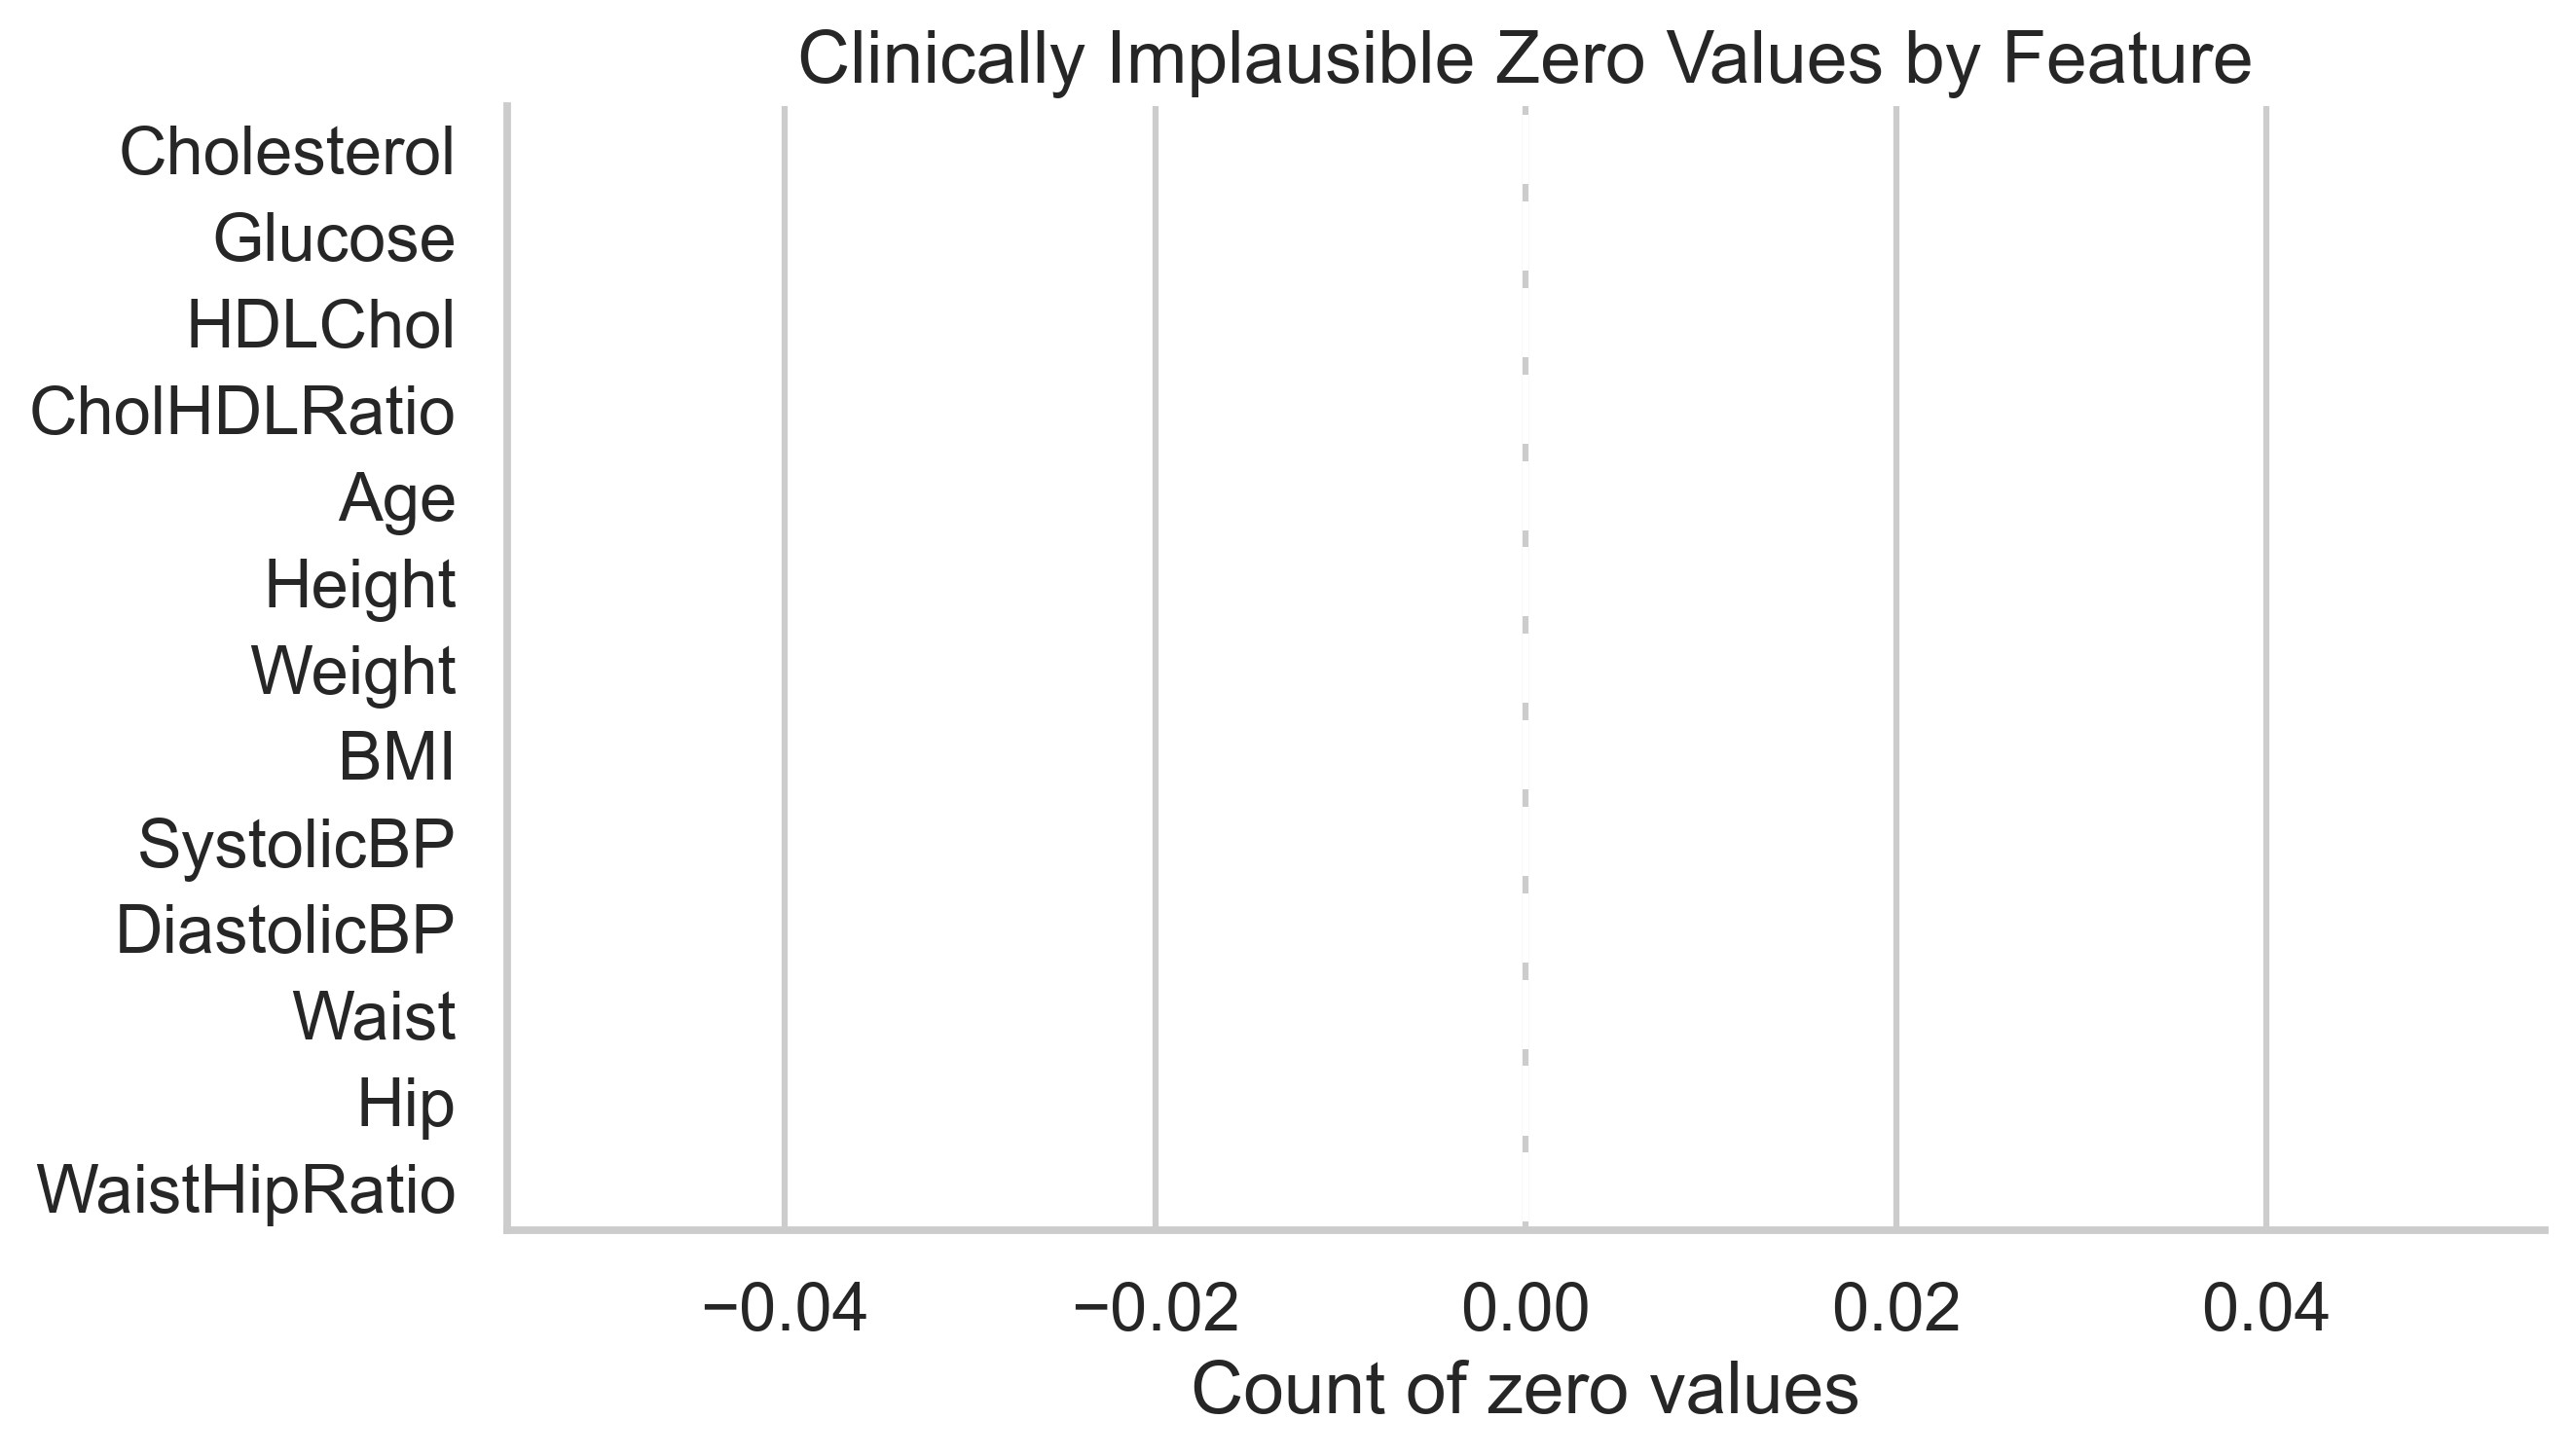
\includegraphics[width=0.88\linewidth]{zero_audit.png}
%     \caption{Audit of suspicious zero values across clinical variables before final modeling. No post-standardization variable required zero-to-missing recoding in the cleaned analytic dataset.}
%     \label{fig:zero-audit}
% \end{figure}

\csvtable{data_quality_summary.csv}{Variable-level missingness summary after ingestion standardization and data cleaning.}{tab:data-quality-summary}
\csvtable{outlier_summary.csv}{Outlier summary based on interquartile-range screening across continuous variables.}{tab:outlier-summary}

\subsection{Exploratory Data Analysis}
Exploratory analysis examined class balance, variable distributions, pairwise relationships, and correlation structure. Particular emphasis was placed on Glucose, BMI, Age, WaistHipRatio, SystolicBP, and DiastolicBP because these variables plausibly reflect the cardiometabolic burden associated with diabetes risk. The class balance summarized in Table~\ref{tab:class-balance} and Fig.~\ref{fig:class-distribution} confirmed a moderately imbalanced outcome distribution, while Figs.~\ref{fig:histograms-by-outcome}--\ref{fig:focused-scatter} provided the descriptive context for later regression and clustering findings.

\begin{figure}[!t]
    \centering
    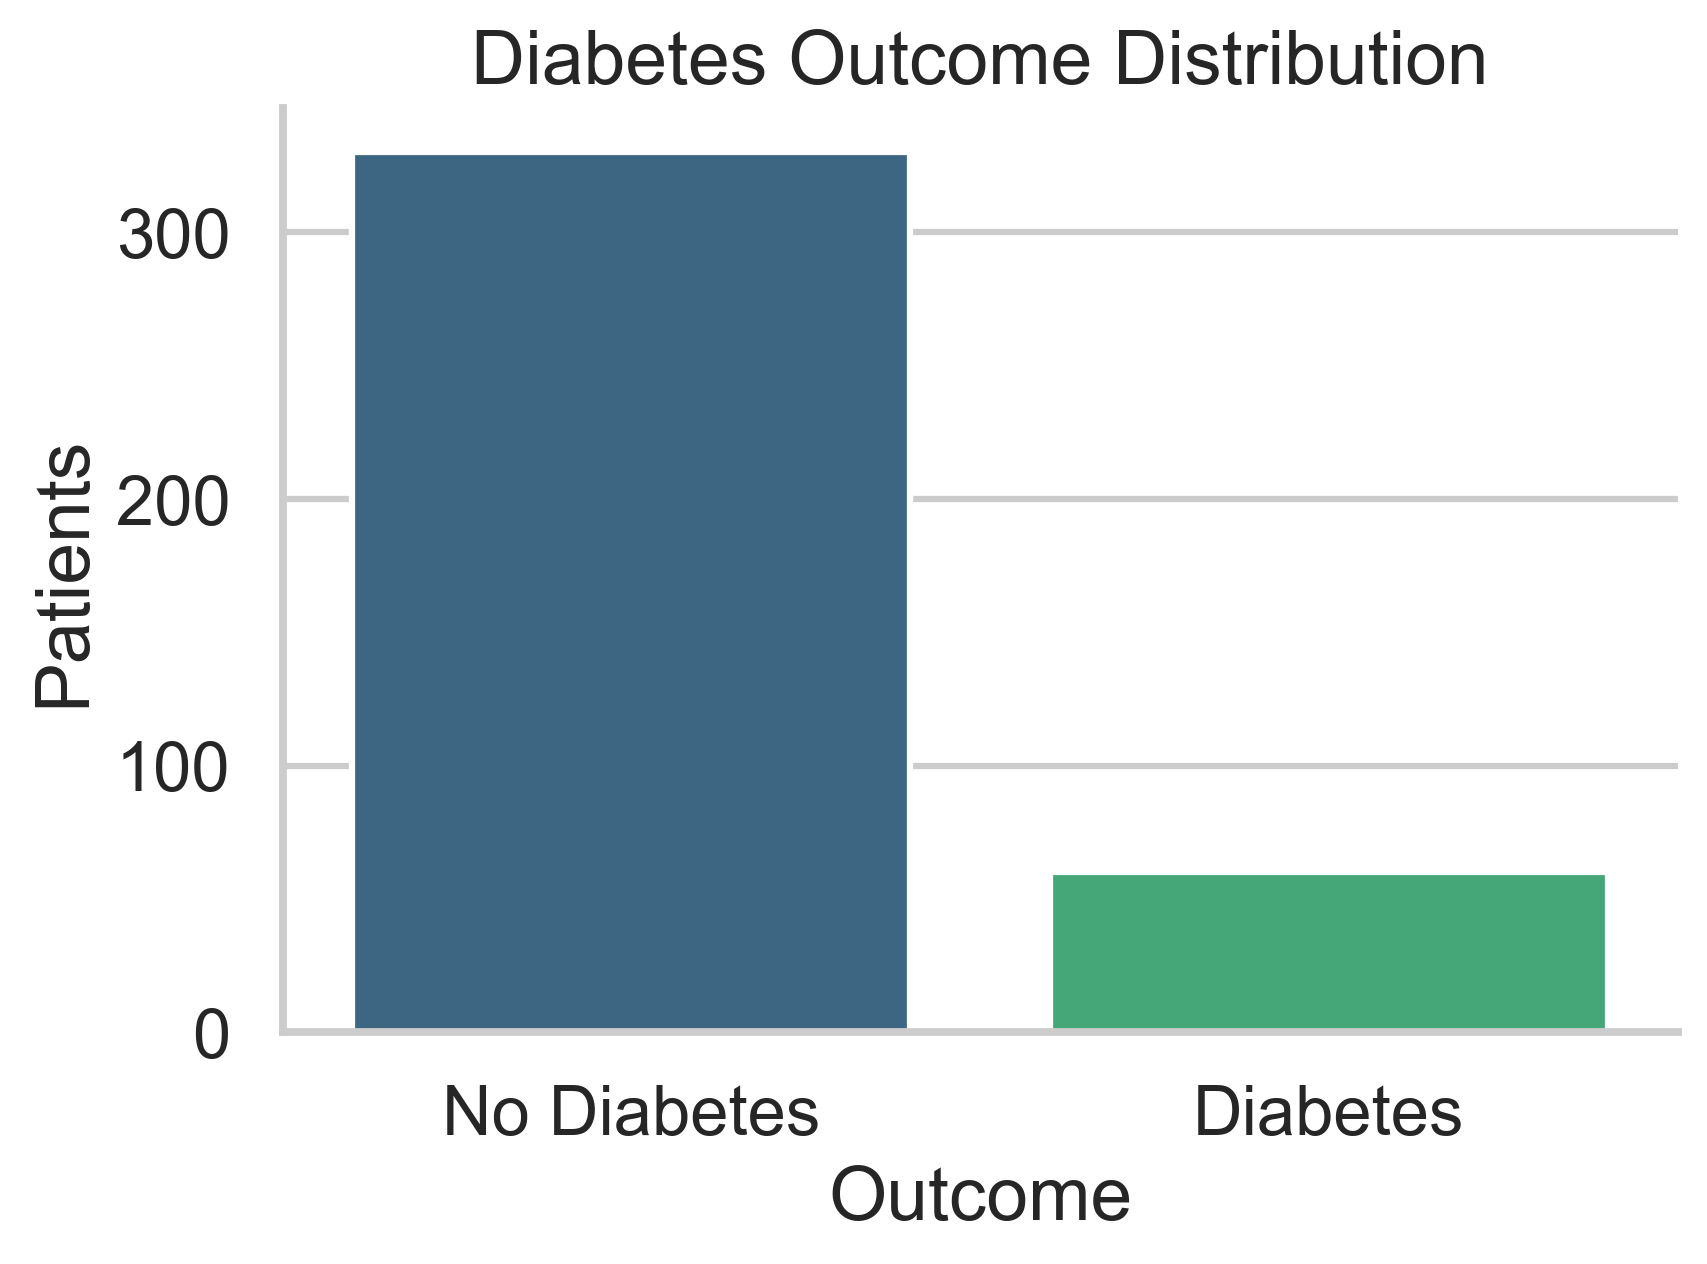
\includegraphics[width=0.62\linewidth]{class_distribution.png}
    \caption{Outcome distribution in the cohort, illustrating the moderate class imbalance that motivates recall-aware evaluation.}
    \label{fig:class-distribution}
\end{figure}

\begin{figure}[!t]
    \centering
    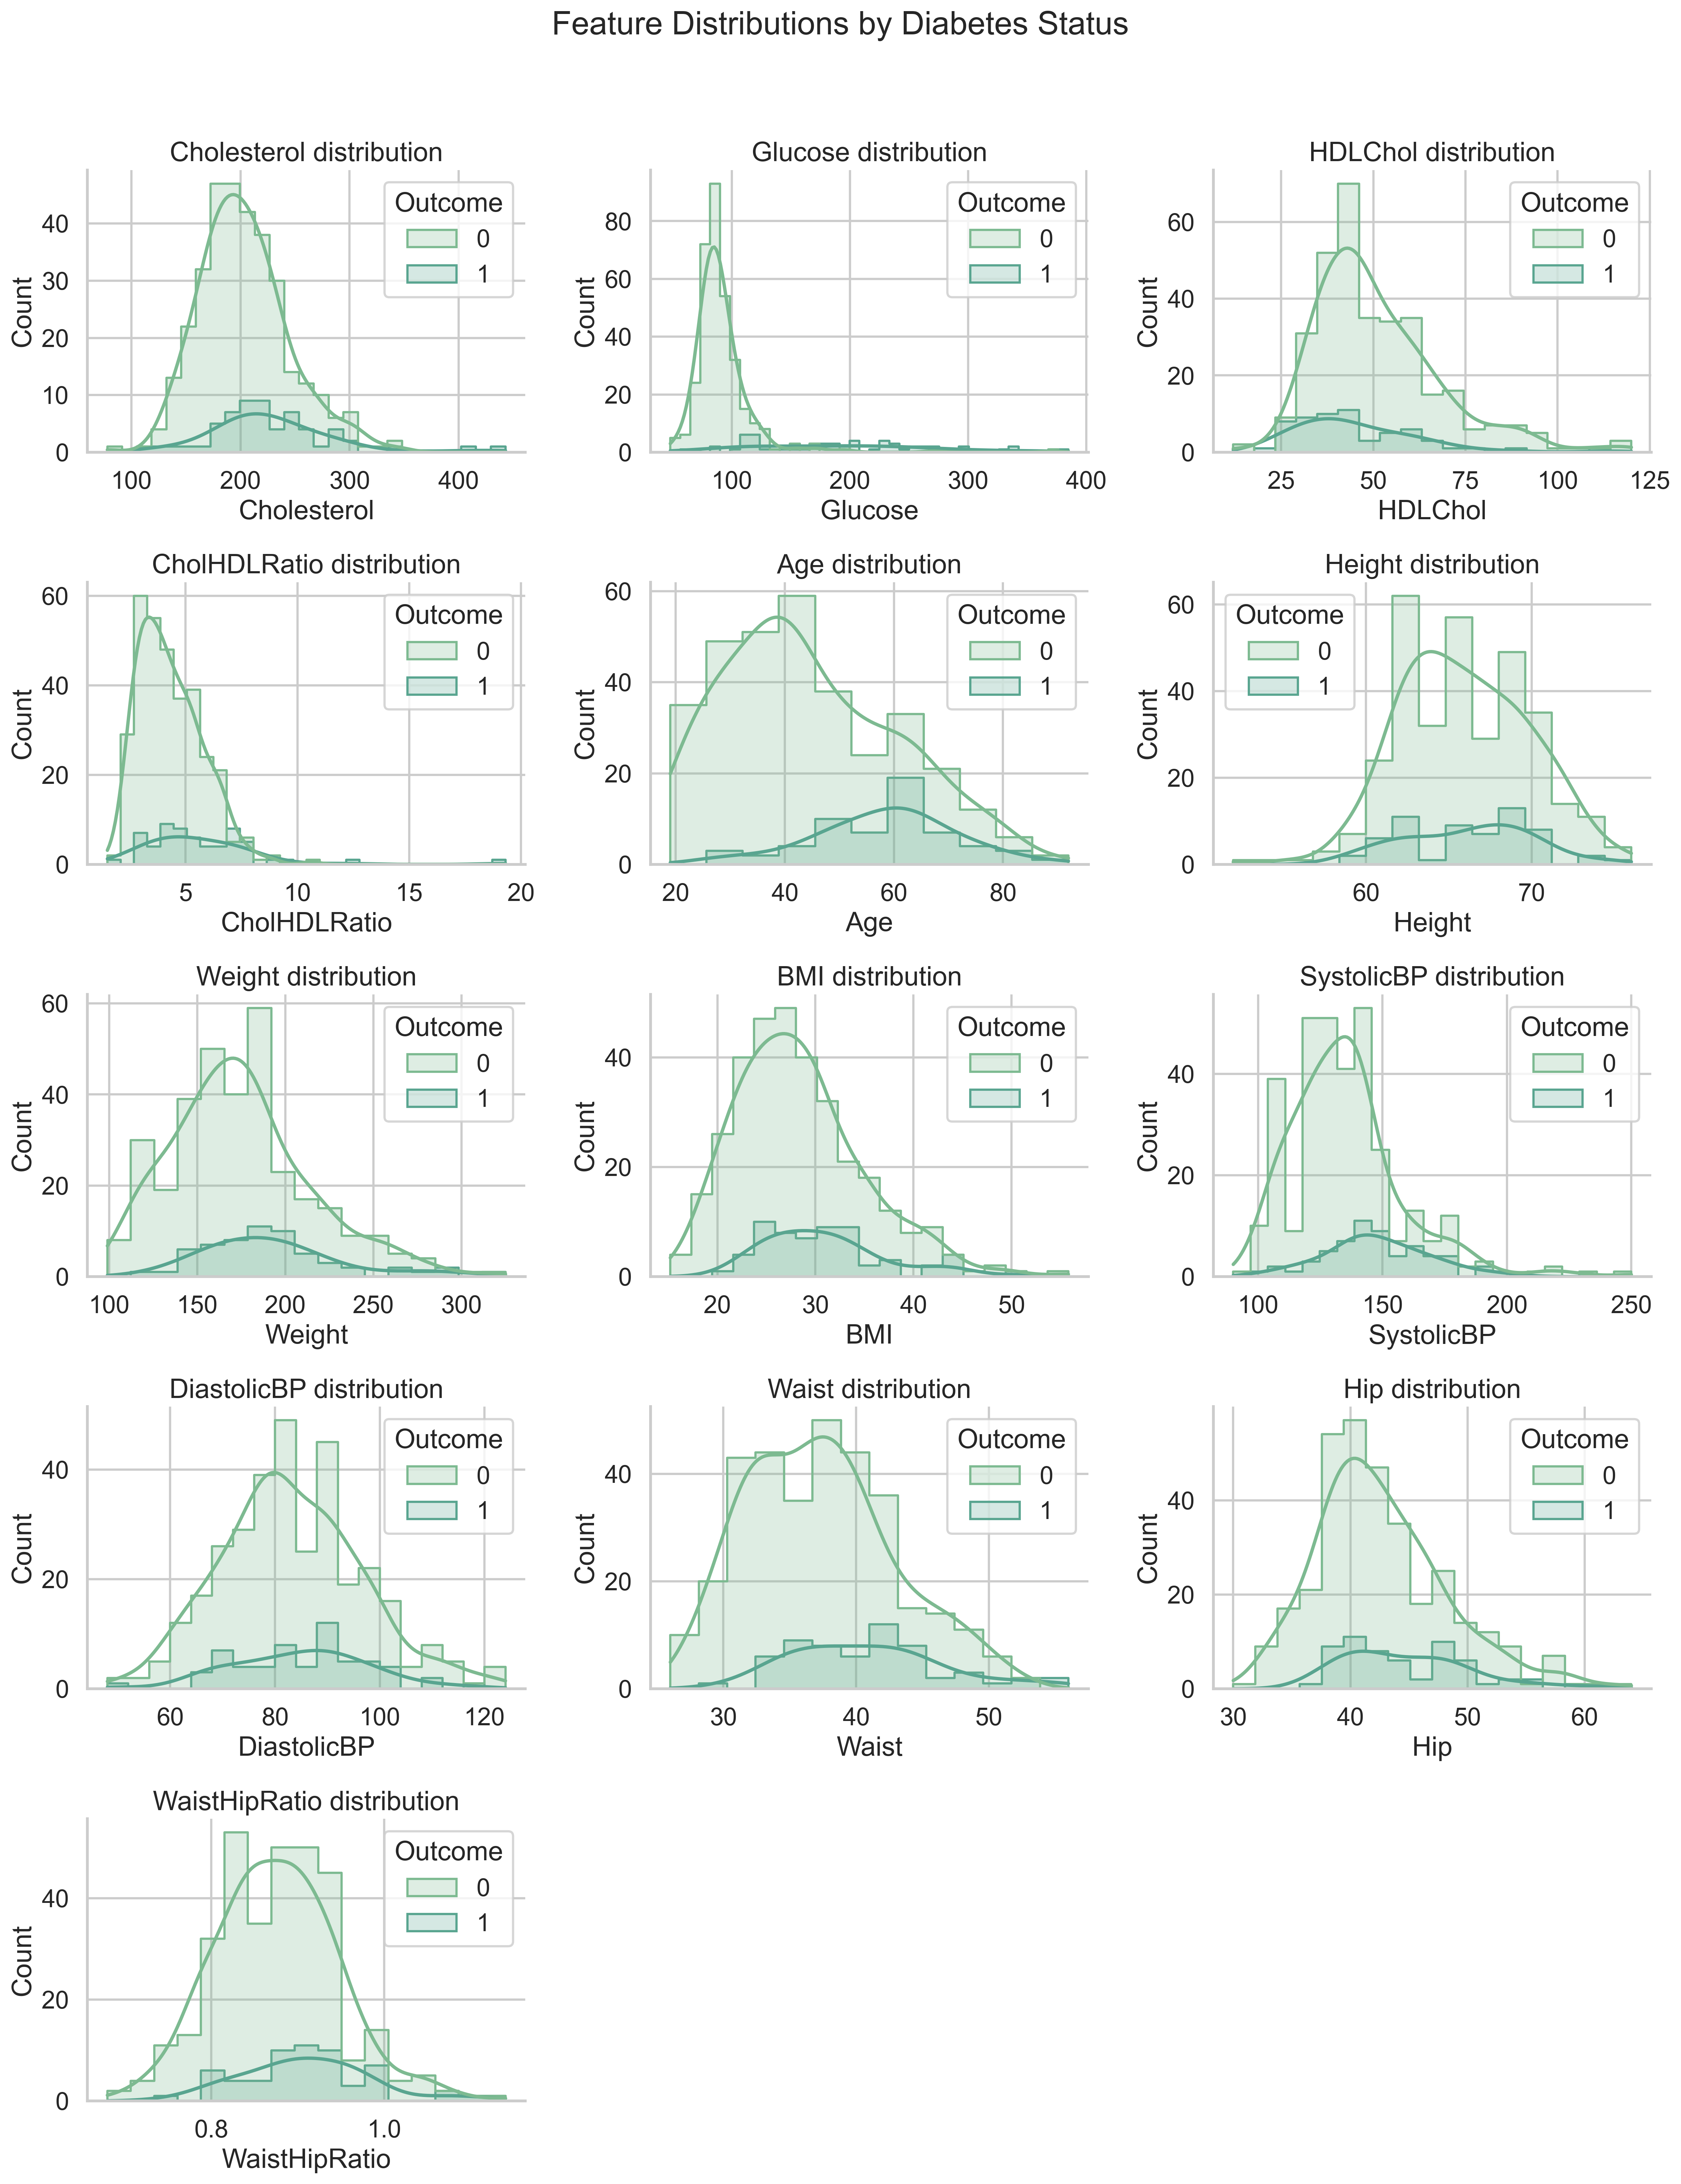
\includegraphics[width=0.95\linewidth]{histograms_by_outcome.png}
    \caption{Distributional comparison of key numeric predictors across Outcome groups.}
    \label{fig:histograms-by-outcome}
\end{figure}

\begin{figure}[!t]
    \centering
    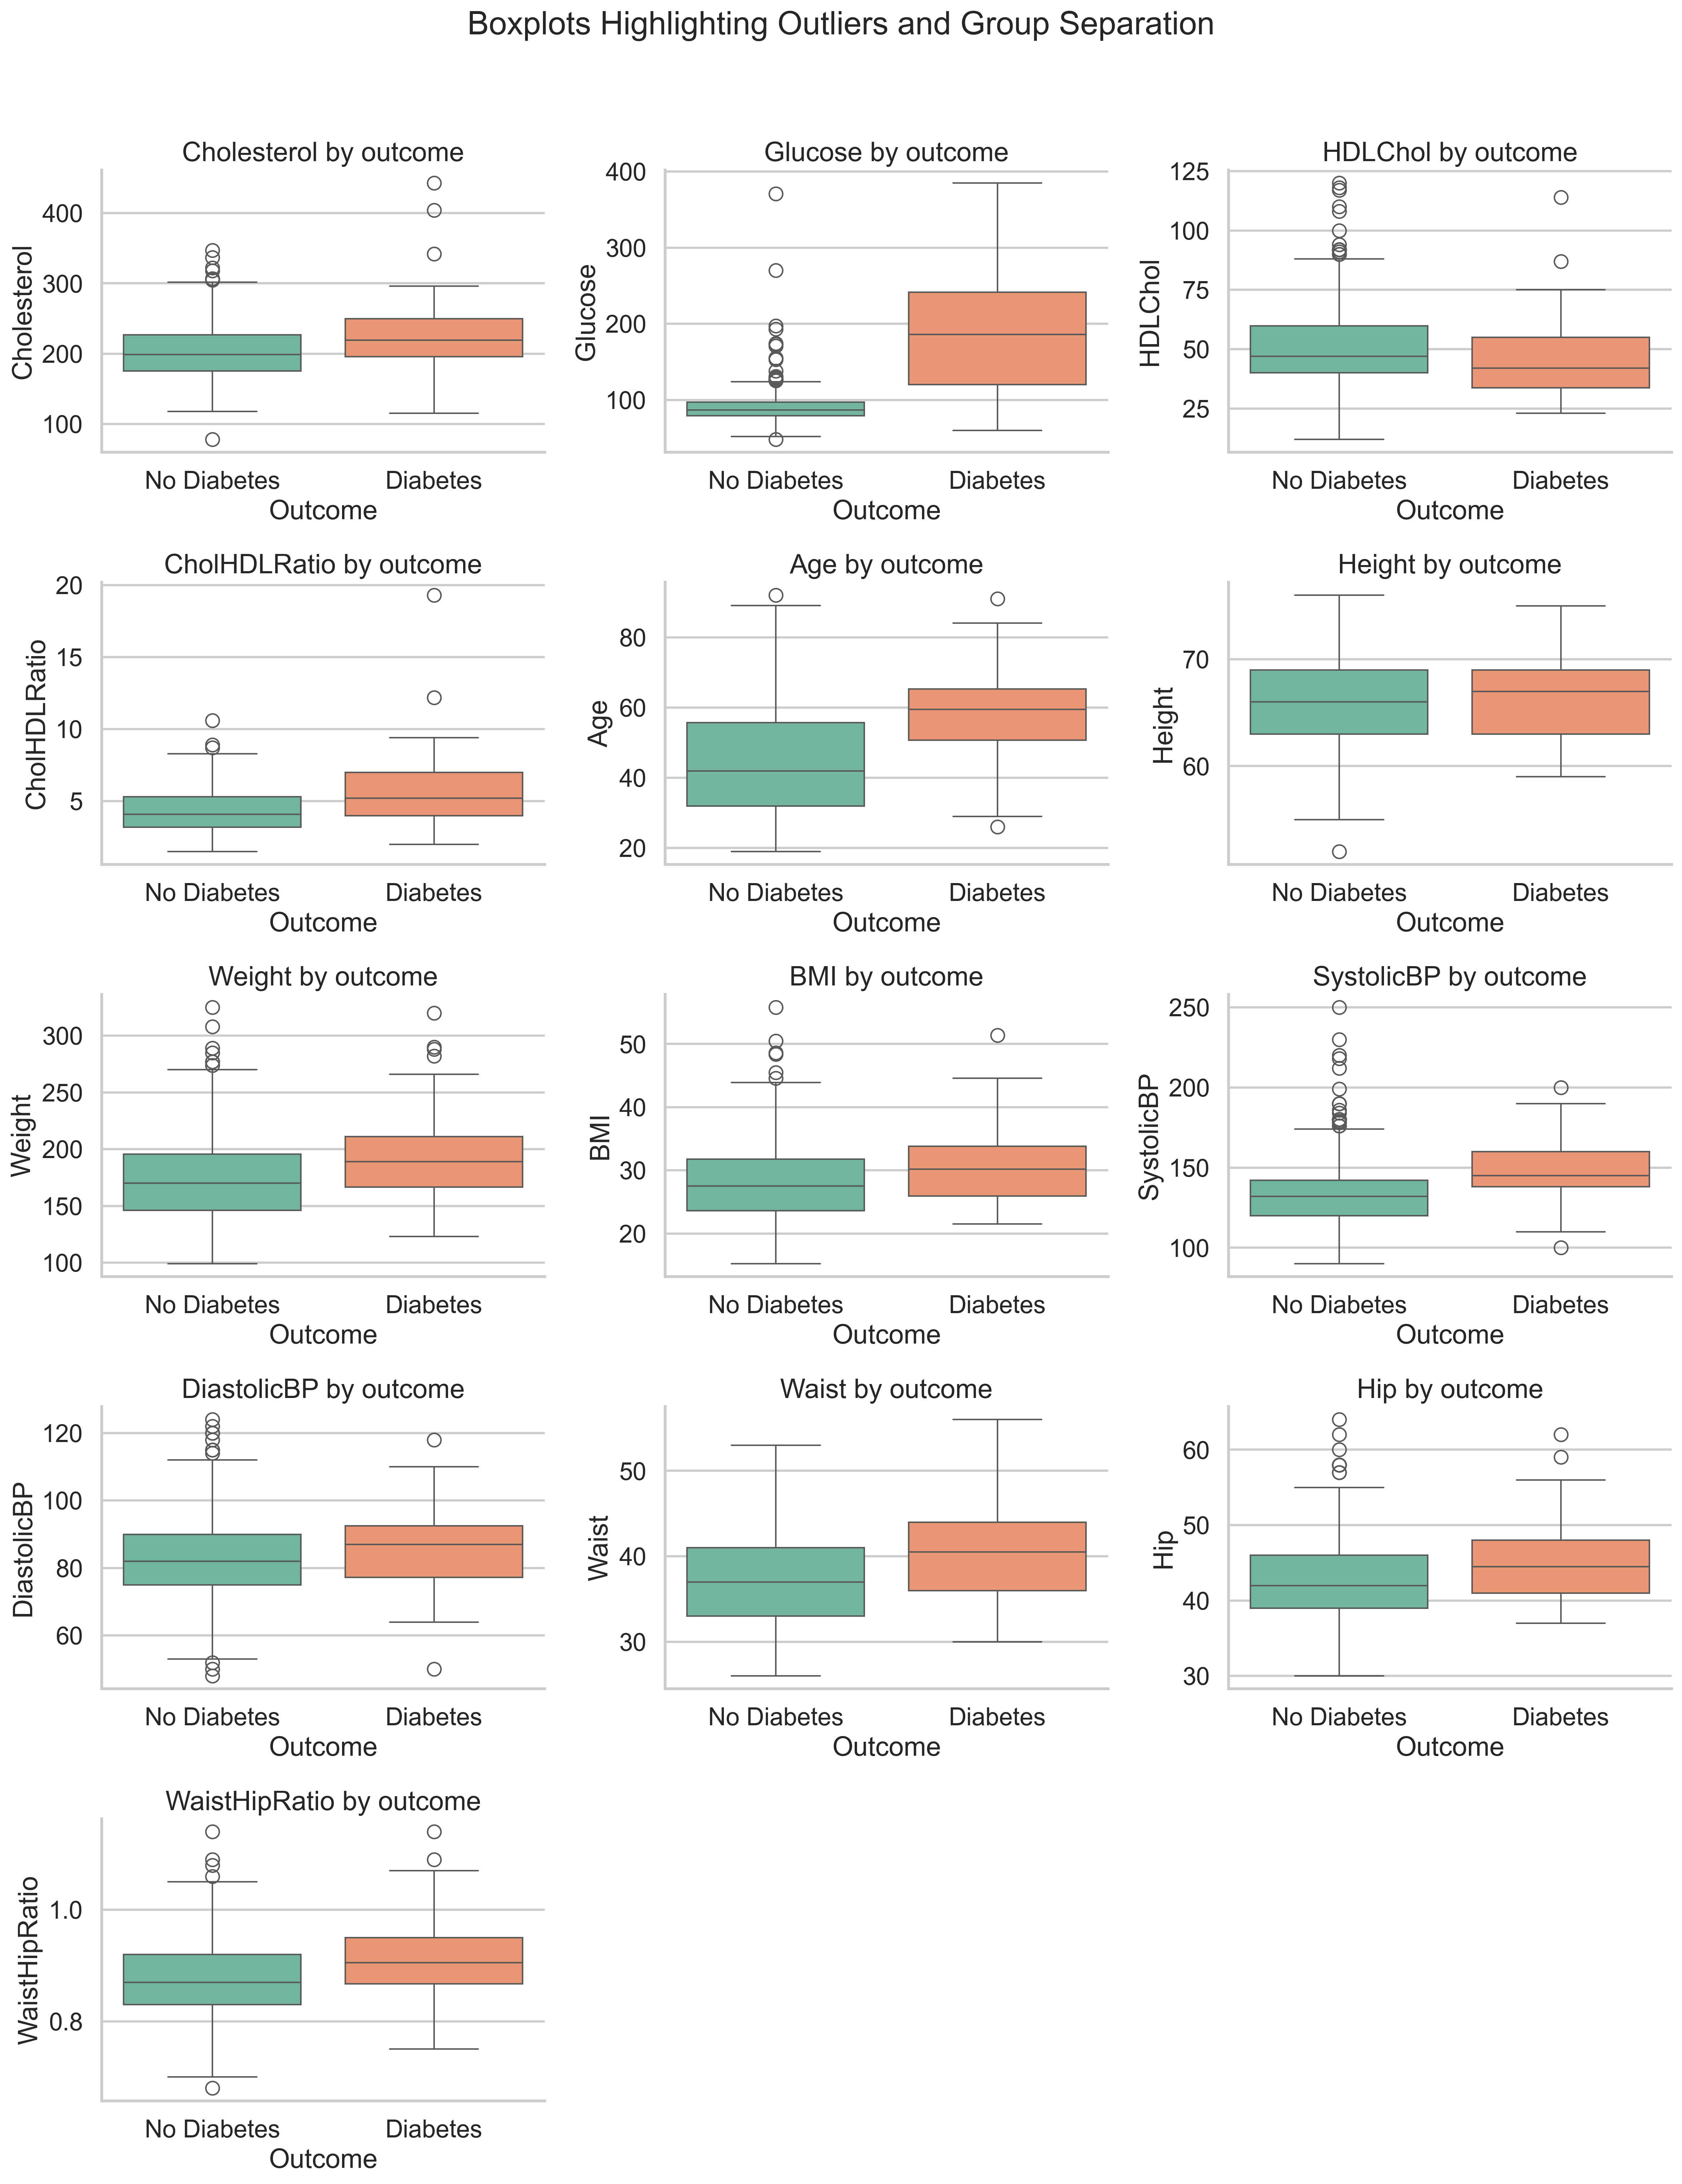
\includegraphics[width=0.95\linewidth]{boxplots_by_outcome.png}
    \caption{Outcome-stratified boxplots highlighting shifts in Glucose, BMI, and blood-pressure-related variables.}
    \label{fig:boxplots-by-outcome}
\end{figure}

\begin{figure}[!t]
    \centering
    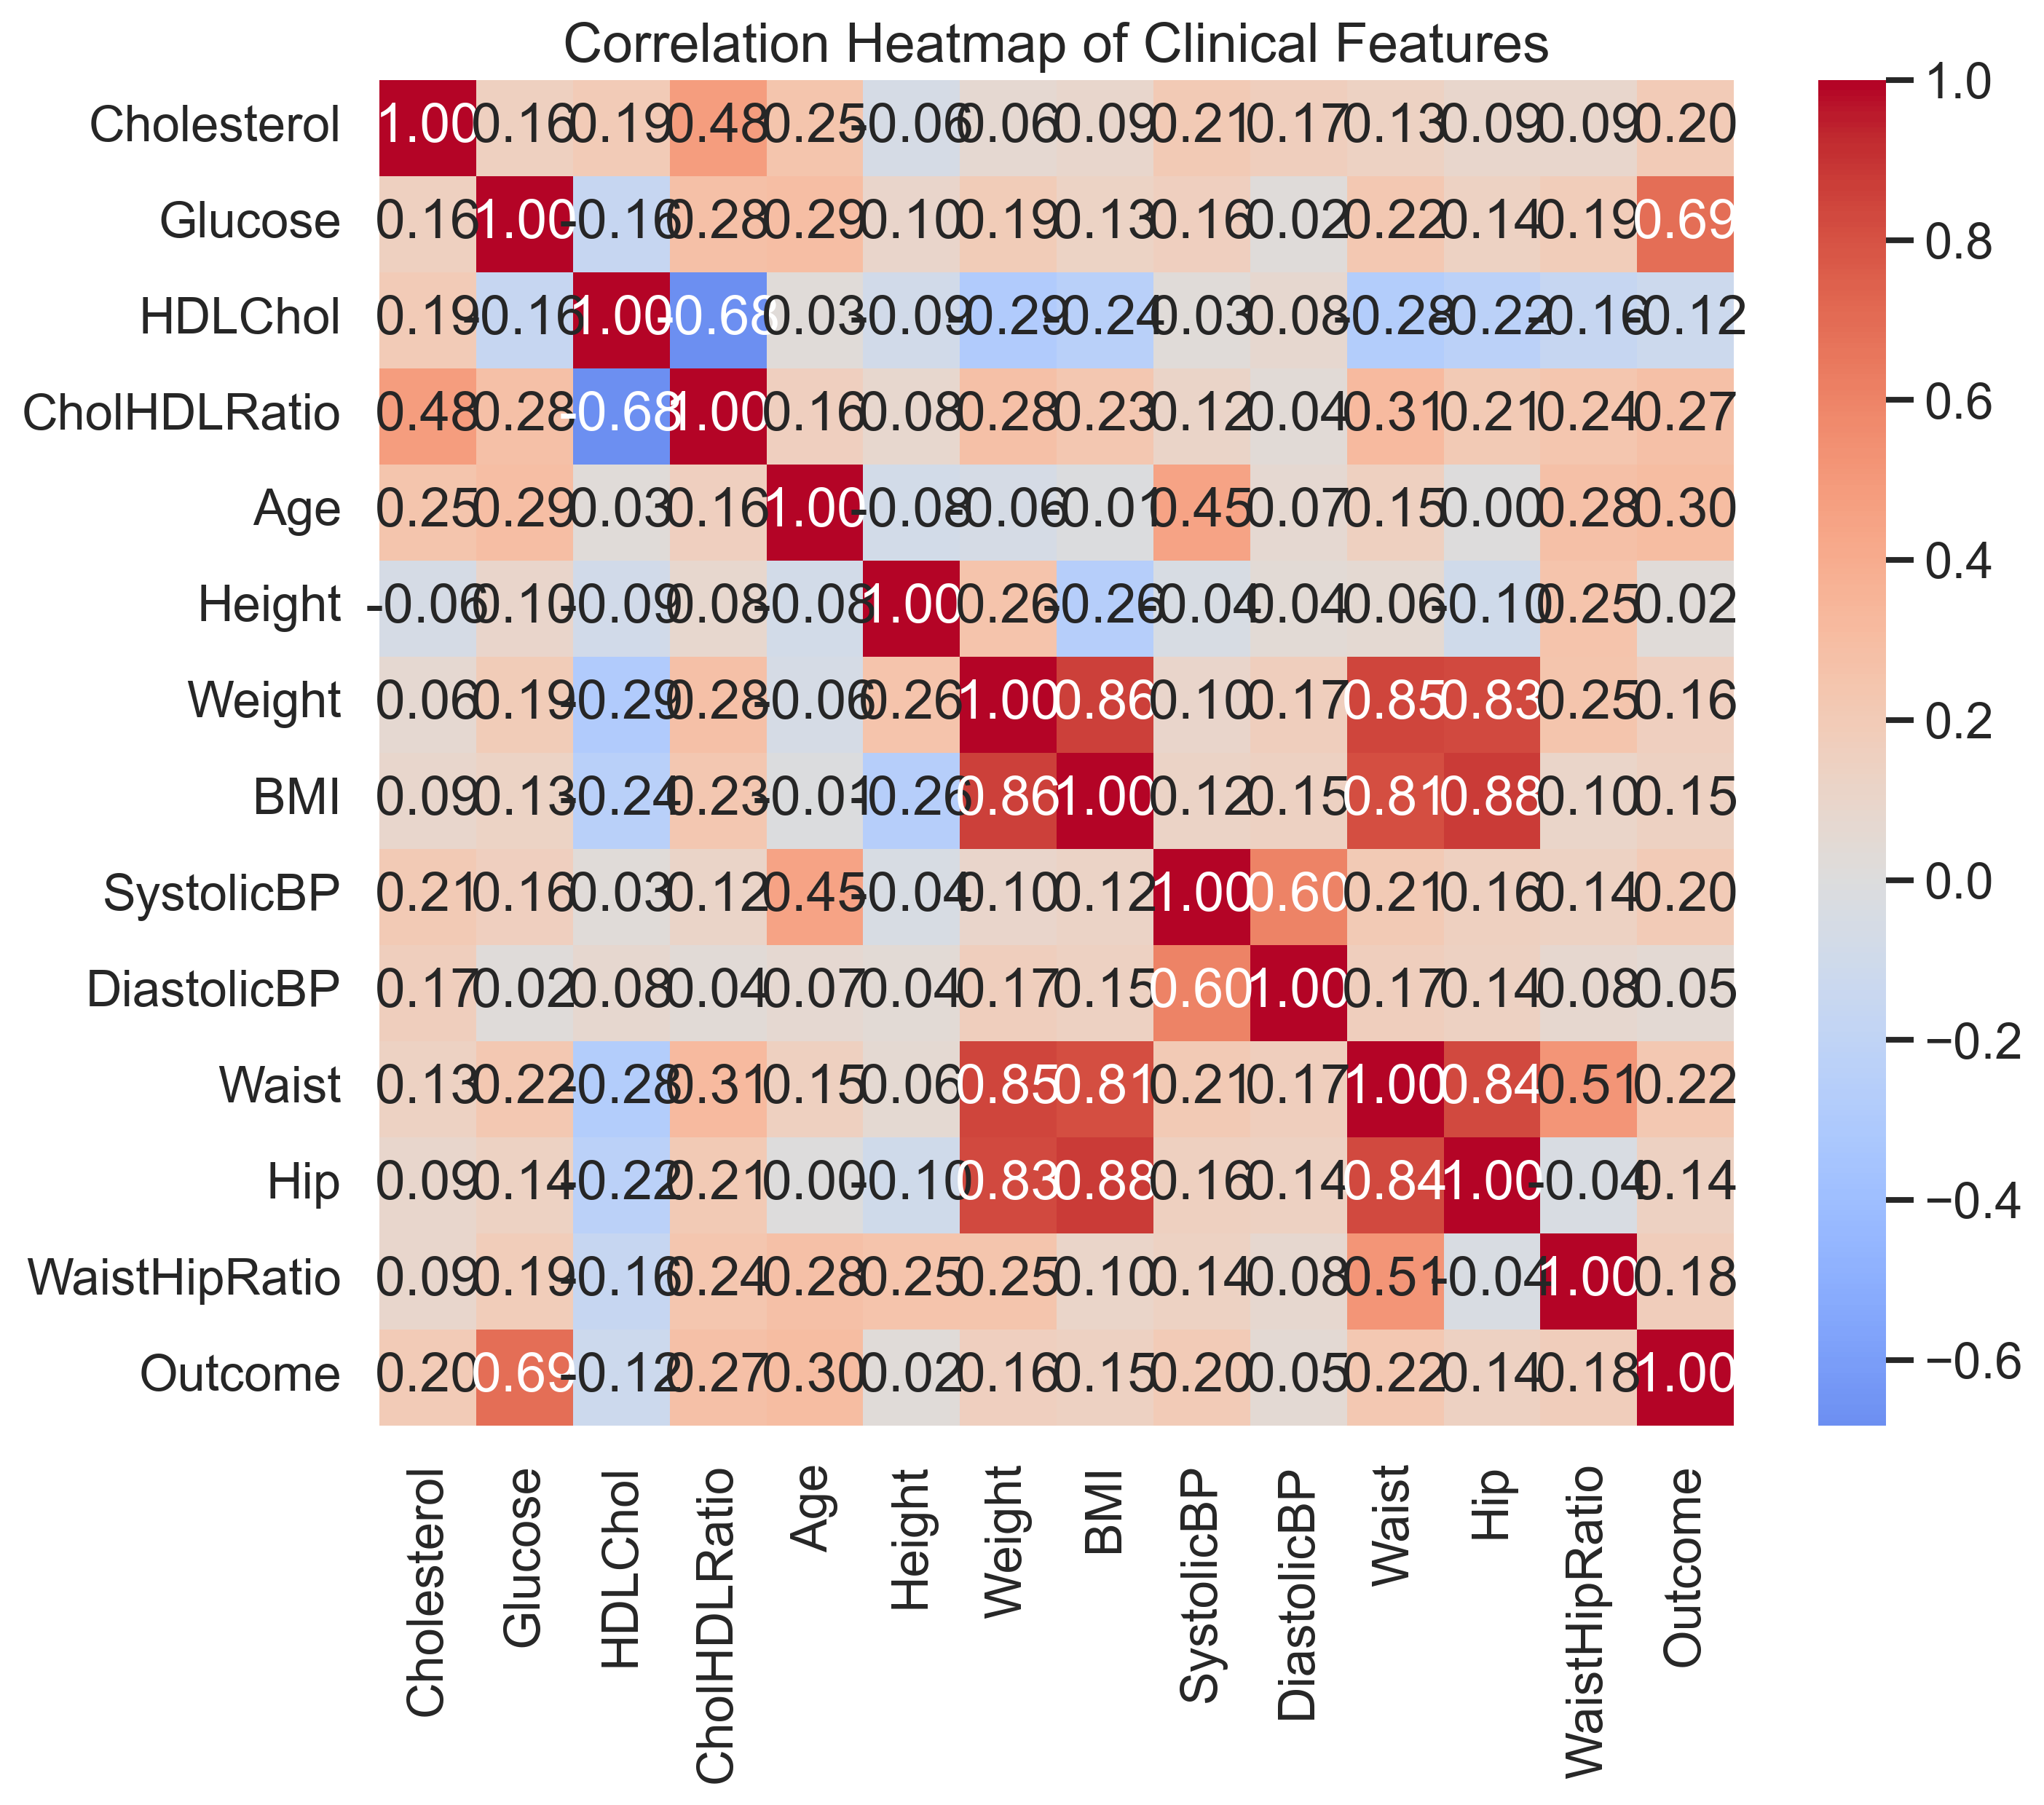
\includegraphics[width=0.9\linewidth]{correlation_heatmap.png}
    \caption{Correlation structure among the continuous predictors used in the healthcare analytics workflow.}
    \label{fig:correlation-heatmap}
\end{figure}

\begin{figure}[!t]
    \centering
    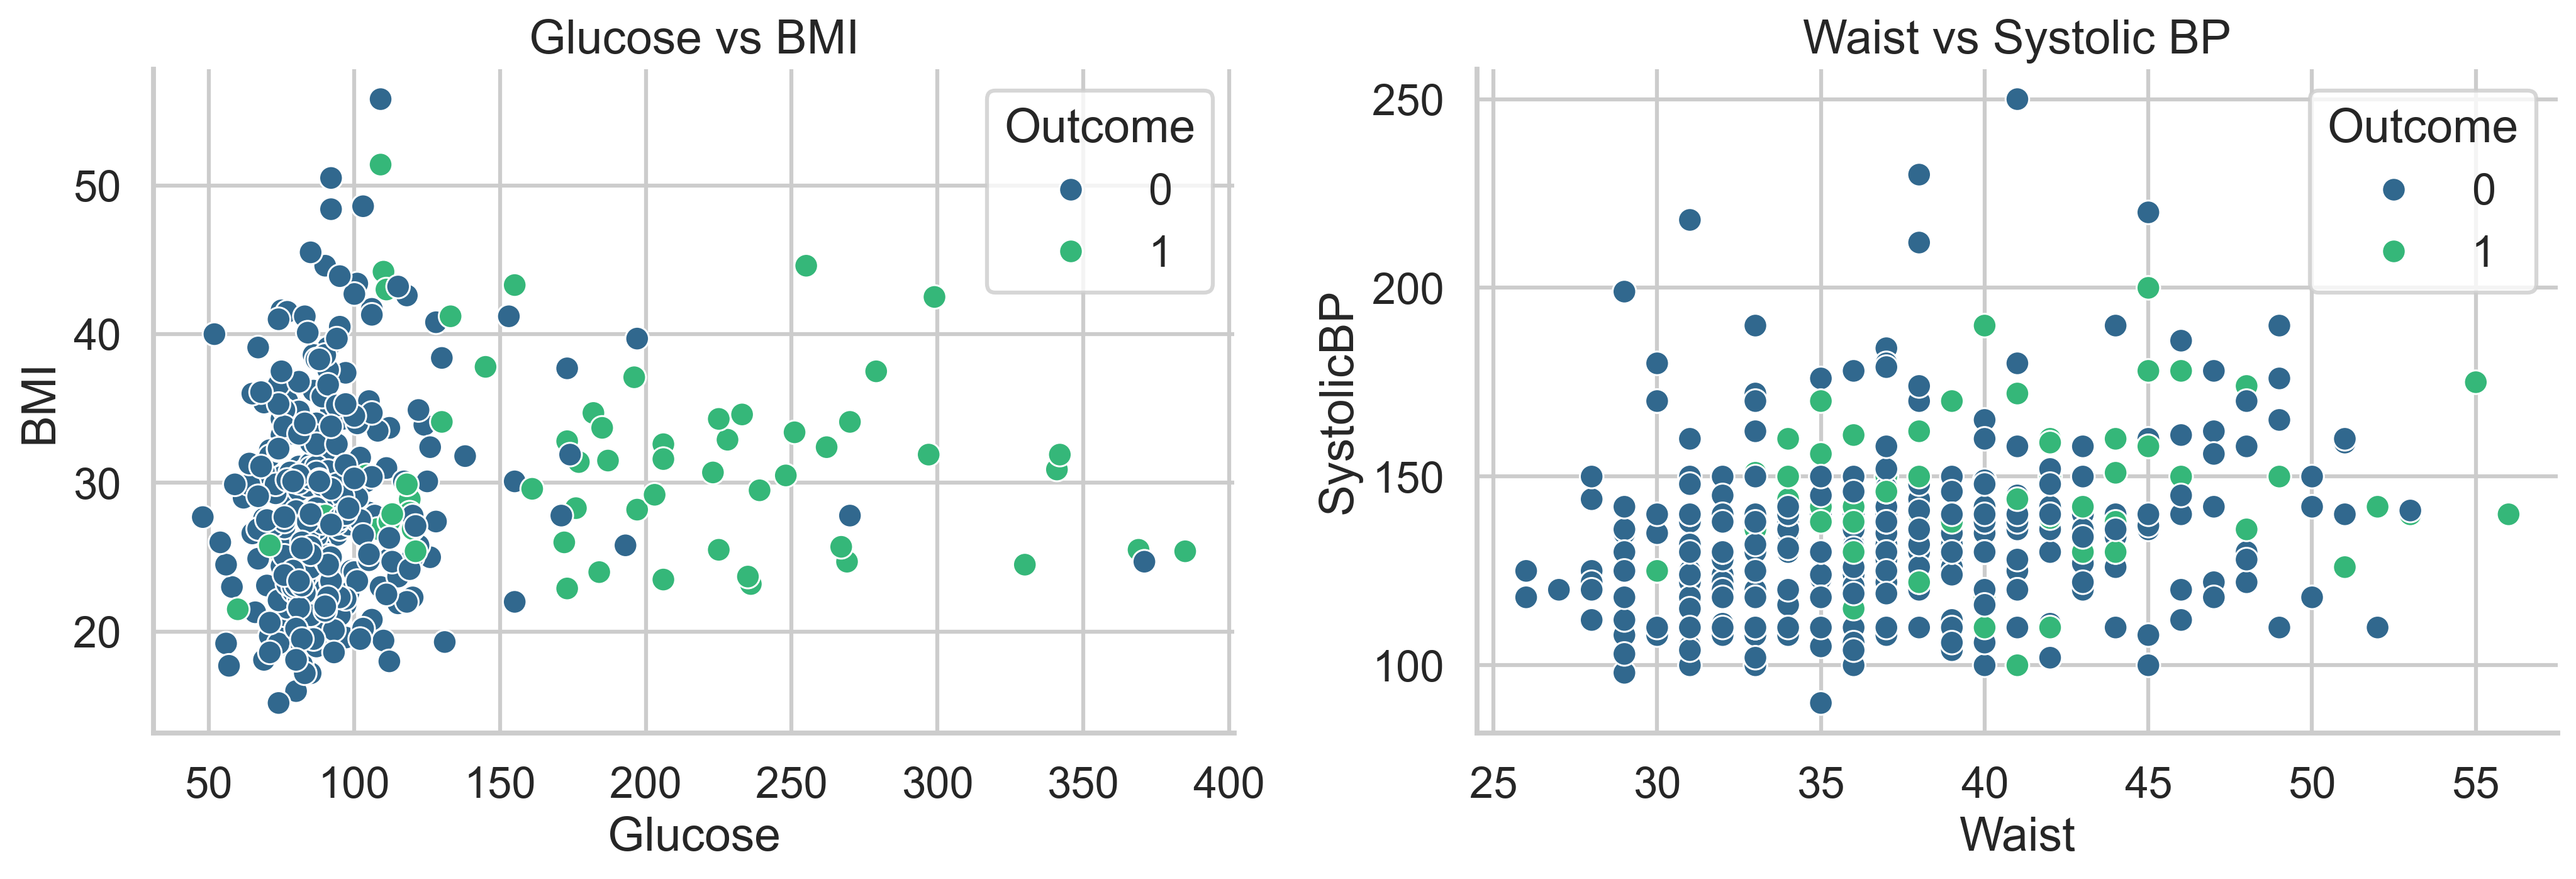
\includegraphics[width=0.9\linewidth]{focused_scatter_panel.png}
    \caption{Focused pairwise relationships among selected metabolic and anthropometric predictors.}
    \label{fig:focused-scatter}
\end{figure}

\csvtable{class_balance.csv}{Observed class balance in the cleaned diabetes cohort.}{tab:class-balance}

\subsection{Classification Models}
The primary supervised task was binary diabetes classification. Logistic Regression, Random Forest, Support Vector Machine, and XGBoost were compared within leakage-safe pipelines. Hyperparameters were tuned with repeated stratified cross-validation using ROC-AUC as the primary selection metric, and held-out performance was assessed with accuracy, precision, recall, F1-score, ROC-AUC, confusion matrices, and Brier-score-based calibration assessment, reflecting established recommendations for evaluating clinical prediction models \cite{calibration}.

Because the cohort was imbalanced, evaluation emphasized recall and false negatives in addition to discrimination. Threshold tuning was conducted on the selected classifier to identify a screening-oriented operating point that could improve sensitivity while maintaining acceptable precision, an important consideration when missed high-risk cases are clinically costly \cite{calibration}. A SMOTE-based sensitivity analysis was also applied to the selected classification family to determine whether oversampling improved recall without materially degrading discrimination or calibration.

\subsection{Regression Models}
To extend the analysis beyond binary classification, Glucose was modeled as a continuous target using the remaining predictors. Linear Regression, Random Forest Regressor, and Gradient Boosting Regressor were compared using repeated cross-validation with negative RMSE as the primary tuning metric. Final evaluation on the held-out set used MAE, MSE, RMSE, and $R^2$.

\subsection{Clustering and Explainability Methods}
Unsupervised clustering was performed with K-Means on standardized numeric predictors. Candidate solutions with $k=2$ to $k=6$ were evaluated using inertia and silhouette scores, and PCA was used only for low-dimensional visualization of the selected structure. Cluster profiling focused on clinically interpretable differences in Glucose, BMI, Age, and OutcomePrevalence, following prior work showing that data-driven subgroup discovery can reveal meaningful heterogeneity in diabetes populations \cite{cluster_diabetes}.

Explainability was examined at both global and local levels. Model-native importance from the selected classifier supported a rank ordering of influential predictors, and SHAP visualizations were used to summarize the direction and relative magnitude of feature effects across the cohort and for an illustrative patient-level prediction \cite{xai_healthcare,xai_shap,xai_ehr}.

\section{Results}

\subsection{Classification Results}
Logistic Regression achieved the strongest held-out ROC-AUC at 0.9798, together with accuracy of 0.9103, precision of 0.7778, recall of 0.5833, and an F1-score of 0.6667. Its Brier score of 0.0522 also indicated good probability quality, which is relevant because both discrimination and calibration matter in healthcare prediction \cite{calibration}. At the default decision threshold, the model produced 5 false negatives and 2 false positives. Support Vector Machine achieved a slightly lower ROC-AUC of 0.9747, but it offered the stronger recall-sensitive operating point: recall increased to 0.8333, F1-score increased to 0.7407, and false negatives fell to 2, albeit with 5 false positives. This pattern highlights an important screening trade-off between overall discrimination and default-threshold sensitivity \cite{calibration}.

Random Forest achieved the largest repeated-cross-validation ROC-AUC (0.9327) but did not maintain that advantage on the held-out set, suggesting weaker generalization than the simpler linear and kernel-based models. XGBoost likewise remained competitive but did not surpass Logistic Regression on held-out ROC-AUC or calibration. A paired Wilcoxon comparison between Logistic Regression and Support Vector Machine yielded a $p$-value of 0.0595, which is suggestive but not definitive given the modest sample size.

Threshold analysis showed that Logistic Regression could be shifted to a more screening-oriented operating point without changing the model family. As summarized in Table~\ref{tab:recommended-threshold}, a threshold of 0.20 achieved recall of 1.0000, precision of 0.7059, specificity of 0.9242, zero false negatives, and five false positives. The full model comparison is reported in Table~\ref{tab:classification-model-comparison}, while Figs.~\ref{fig:roc-comparison} and~\ref{fig:calibration-curves} illustrate the discrimination and calibration trade-offs across classifiers. The SMOTE sensitivity analysis also increased default-threshold recall to 1.0000, but it reduced precision to 0.5714 and worsened calibration (Brier score 0.0932). Consequently, threshold tuning of the original model was preferred over oversampling for this dataset.

\csvtablewide{classification_model_comparison.csv}{Cross-validated and held-out classification performance for candidate diabetes classifiers.}{tab:classification-model-comparison}

\begin{figure}[!t]
    \centering
    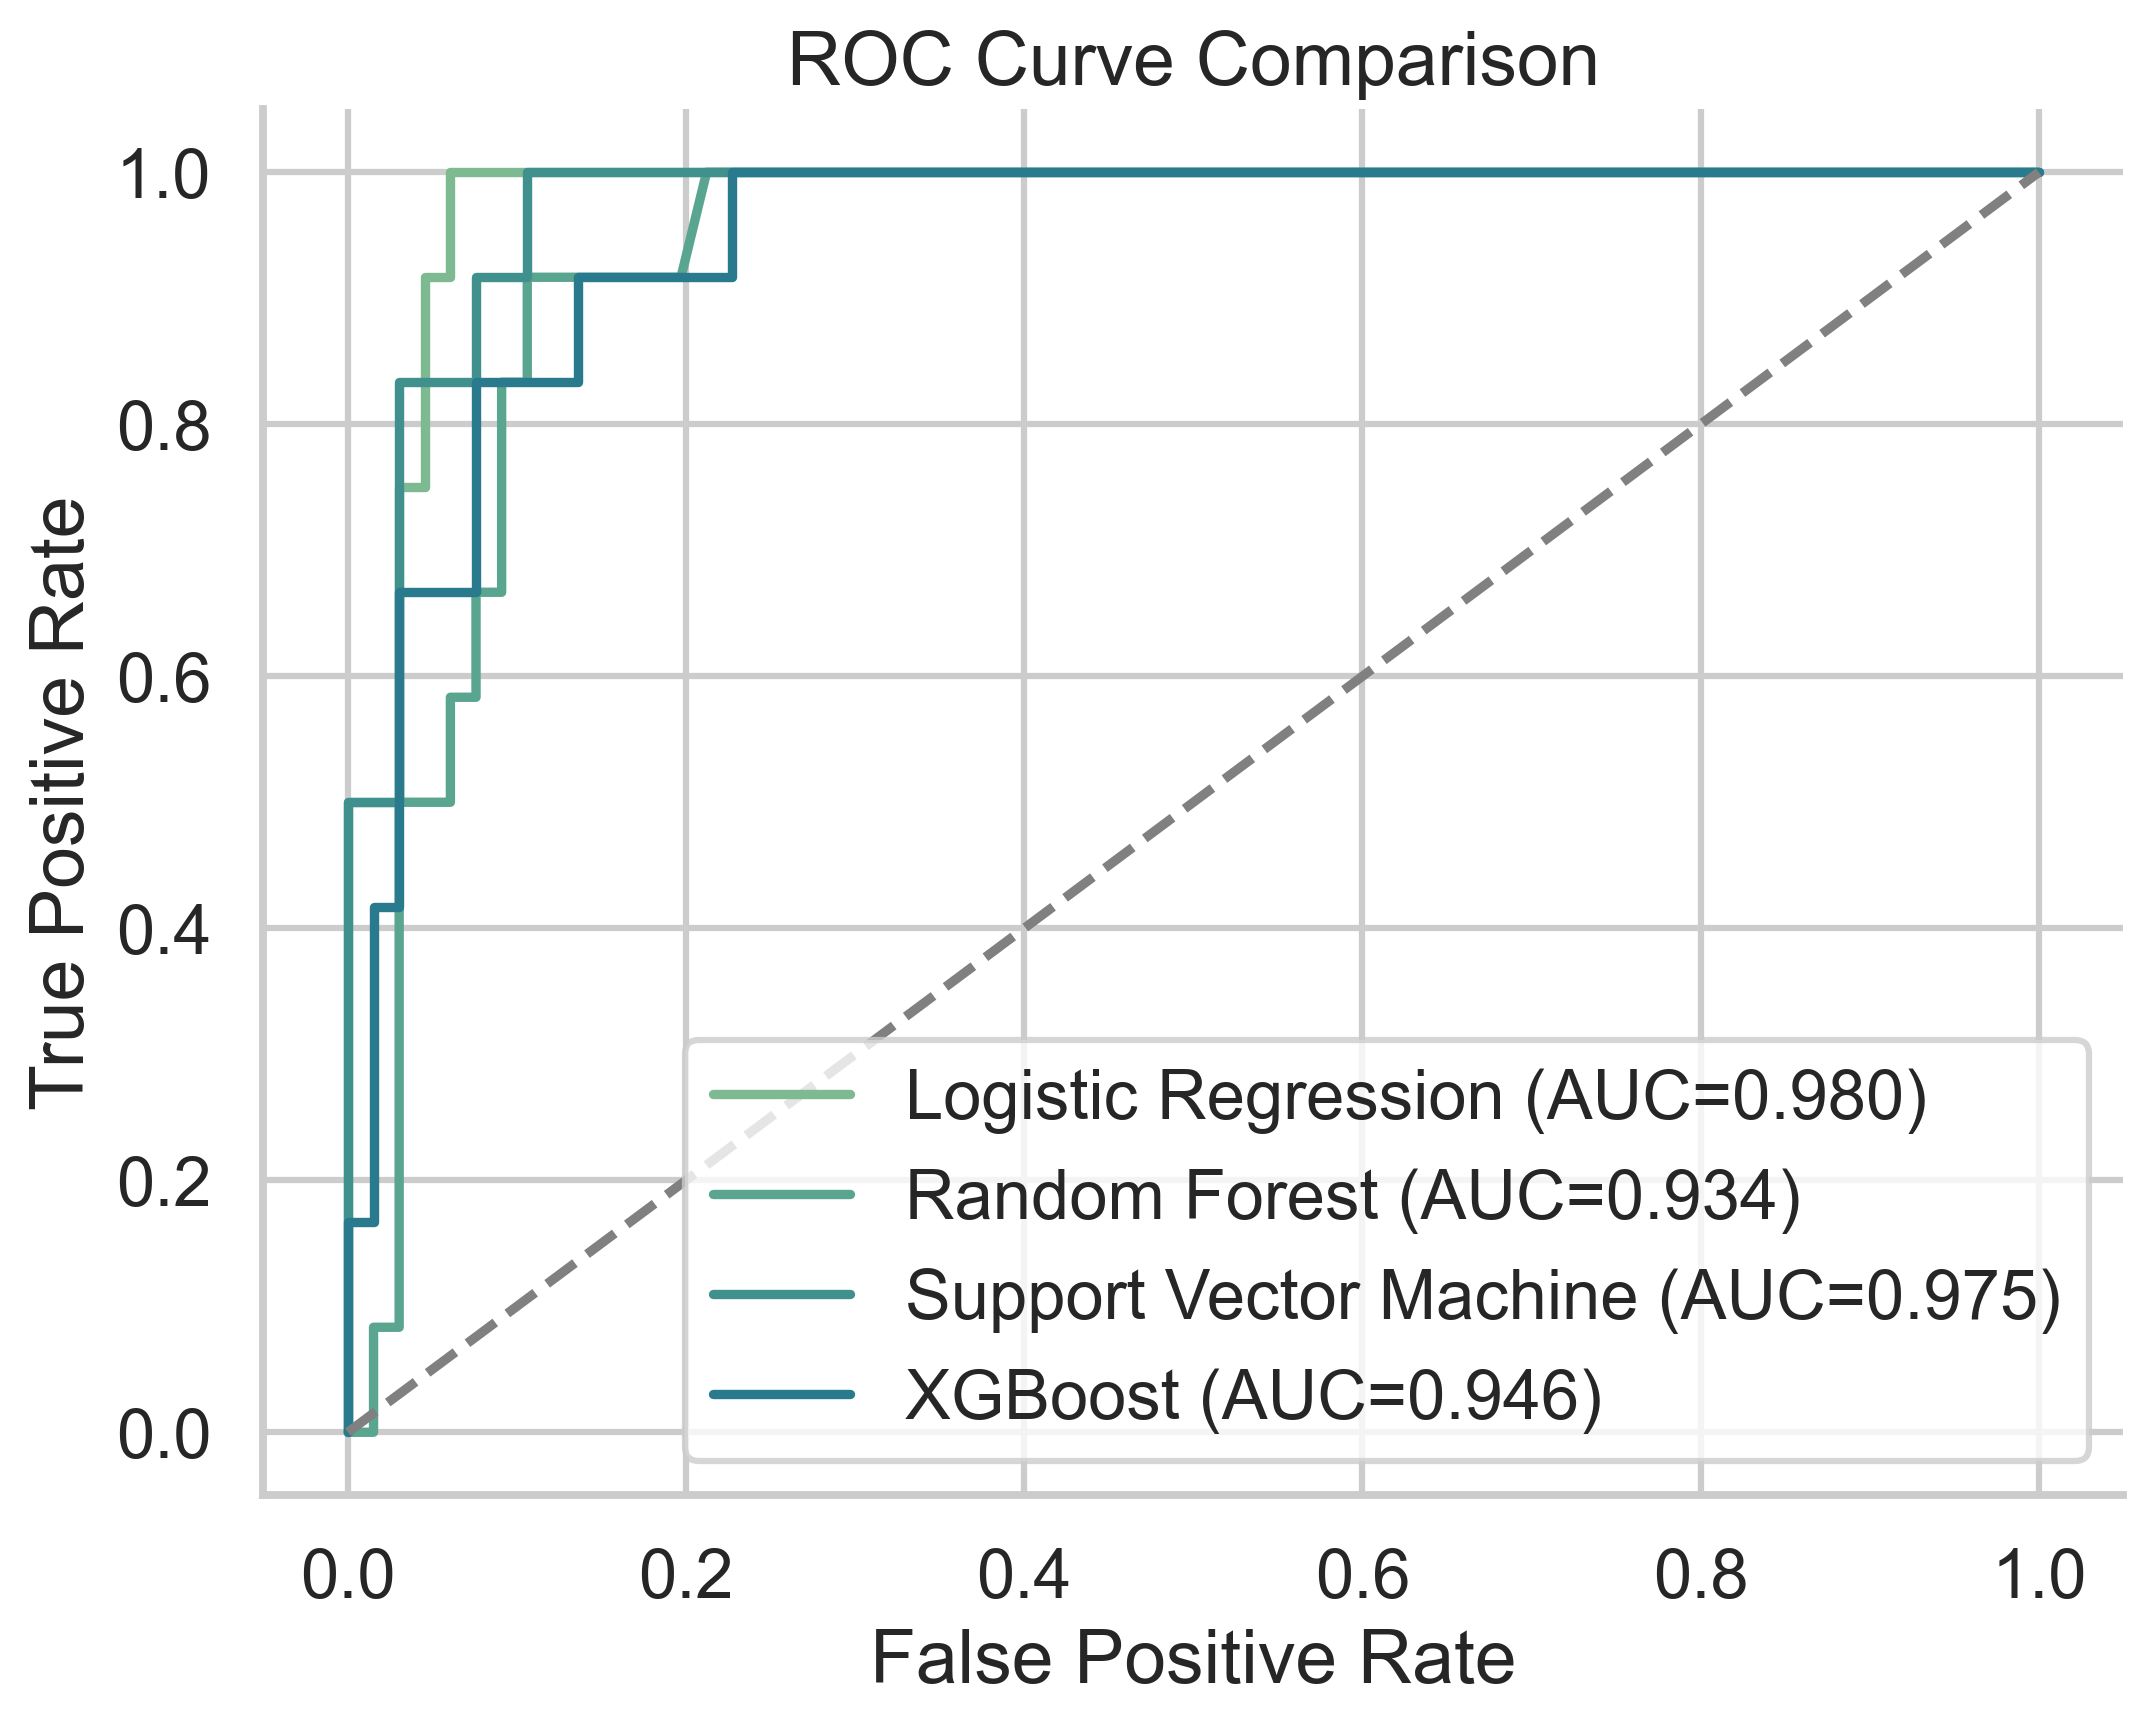
\includegraphics[width=0.88\linewidth]{classification_roc_comparison.png}
    \caption{ROC comparison across candidate classification models on the held-out test set.}
    \label{fig:roc-comparison}
\end{figure}

\begin{figure}[!t]
    \centering
    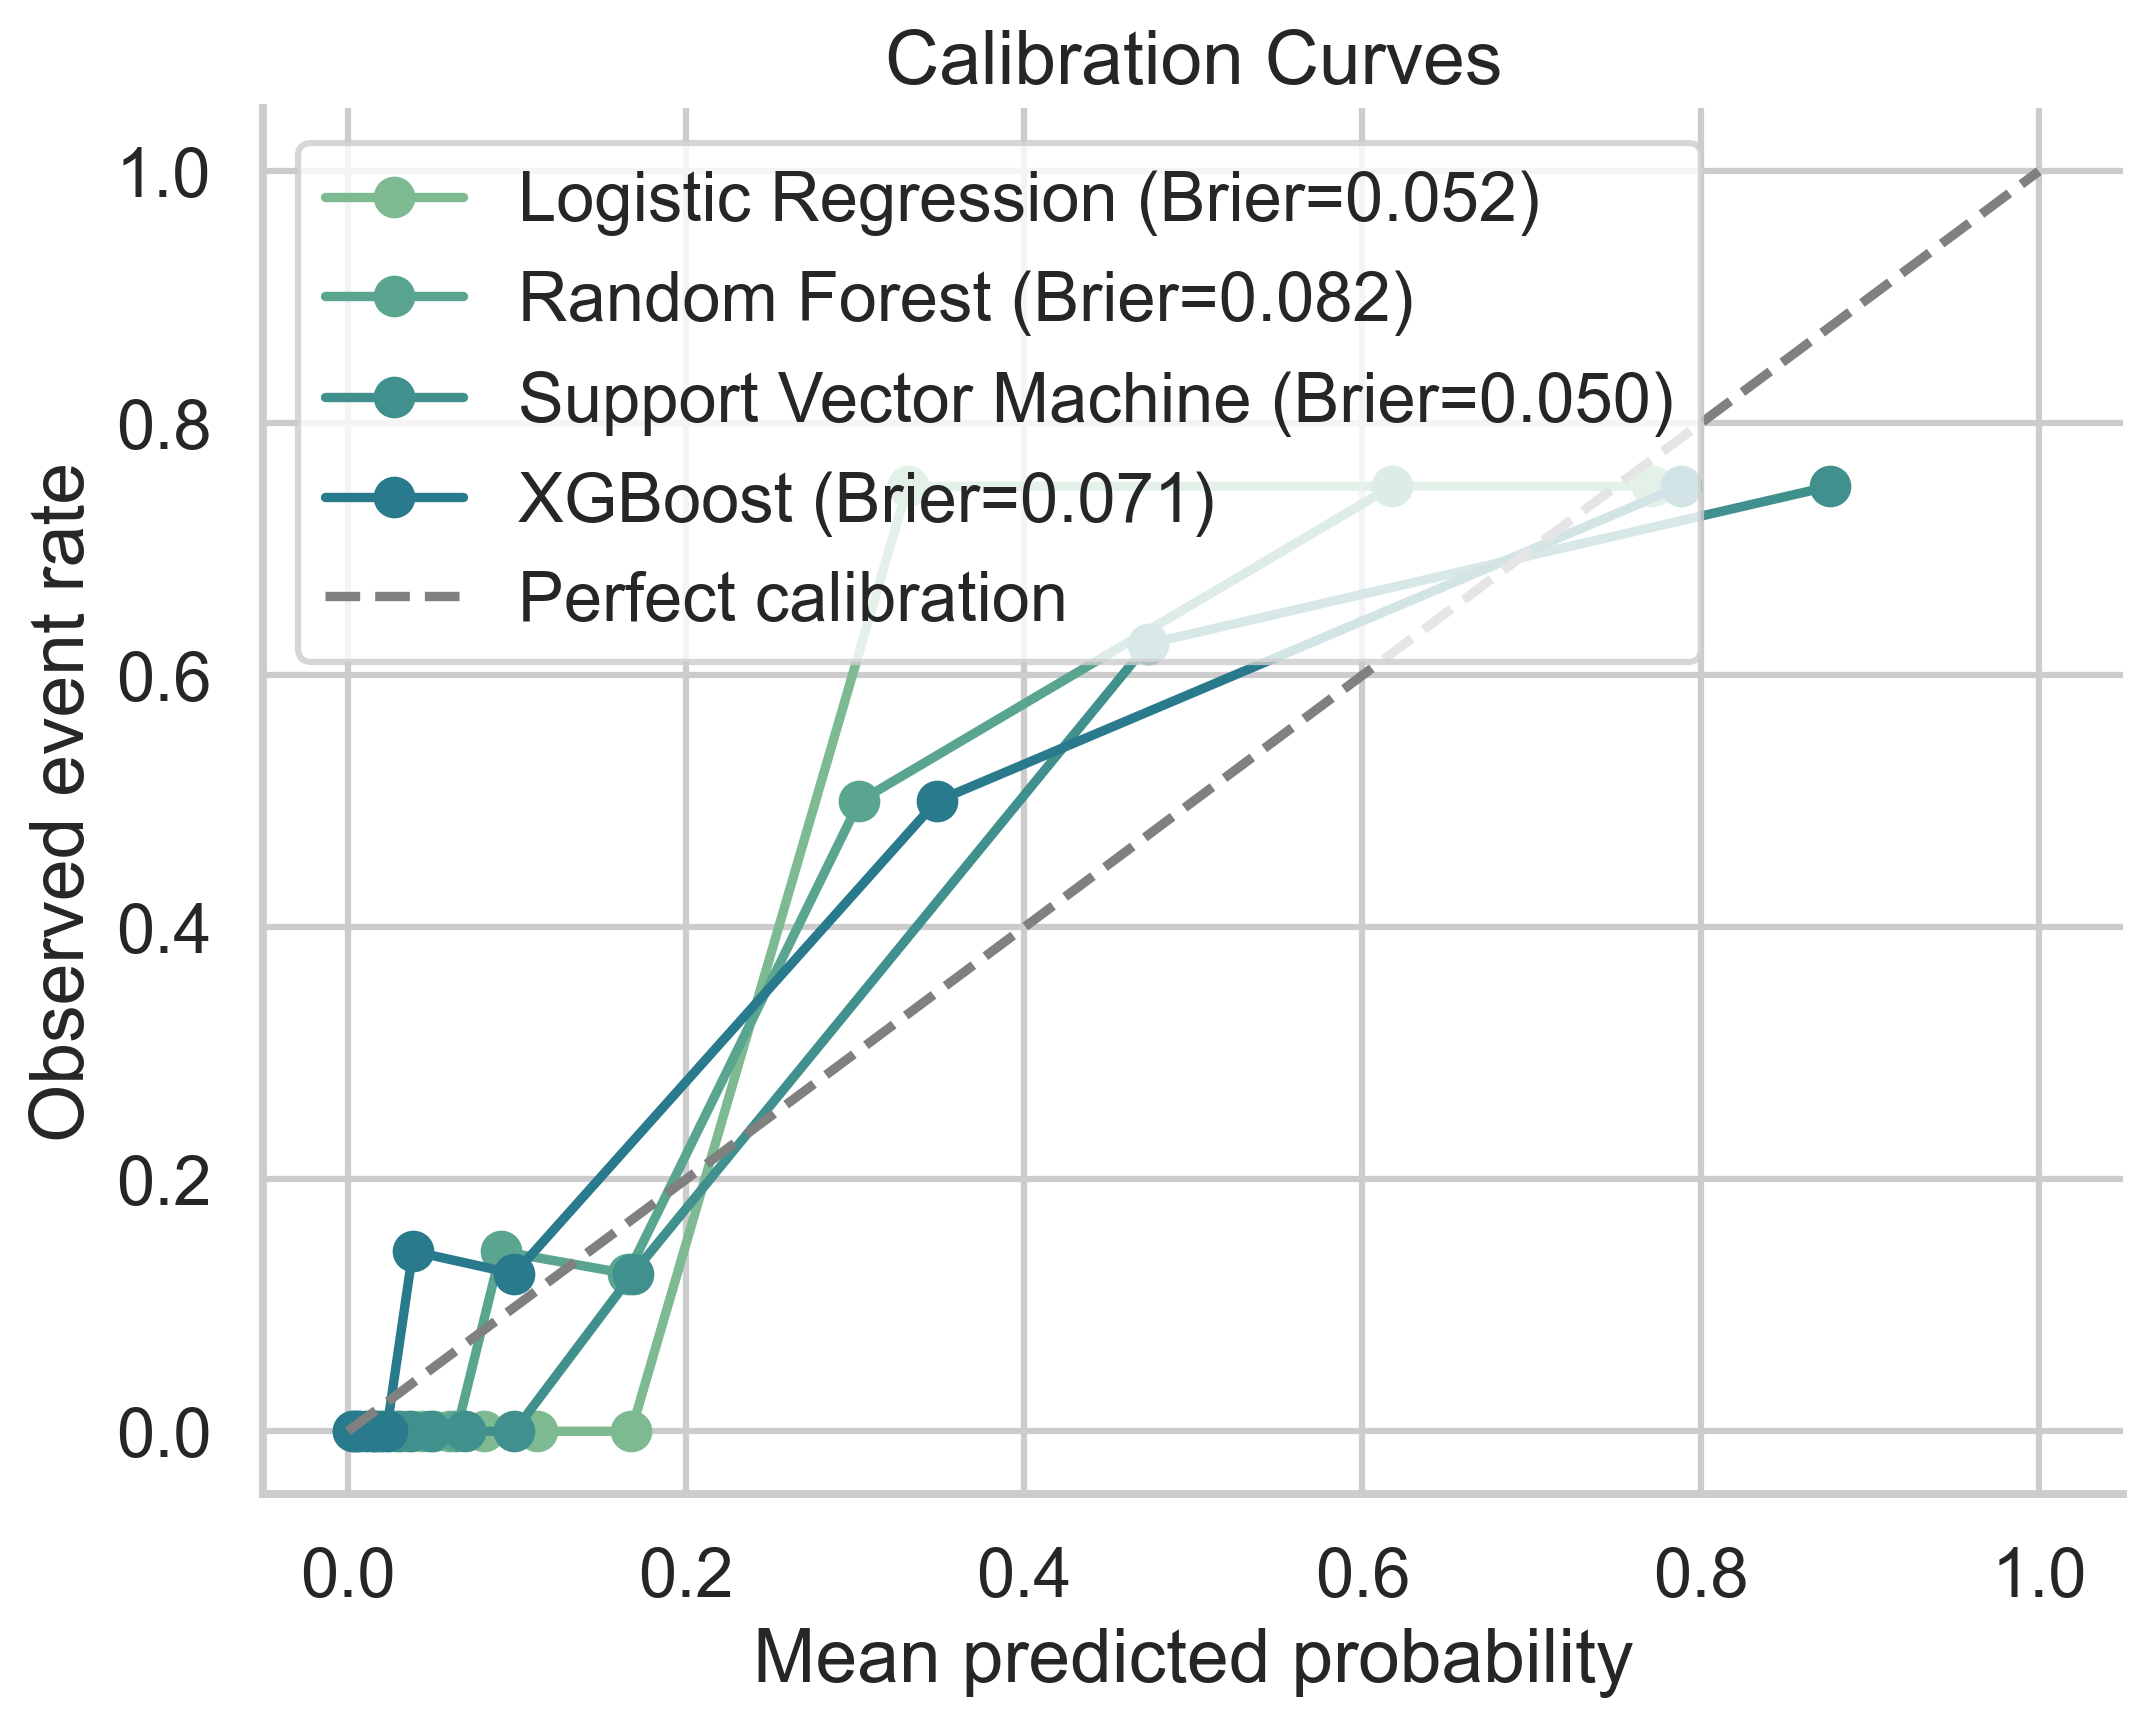
\includegraphics[width=0.88\linewidth]{classification_calibration_curves.png}
    \caption{Calibration curves for candidate classifiers, highlighting agreement between predicted probabilities and observed risk.}
    \label{fig:calibration-curves}
\end{figure}

\begin{figure}[!t]
    \centering
    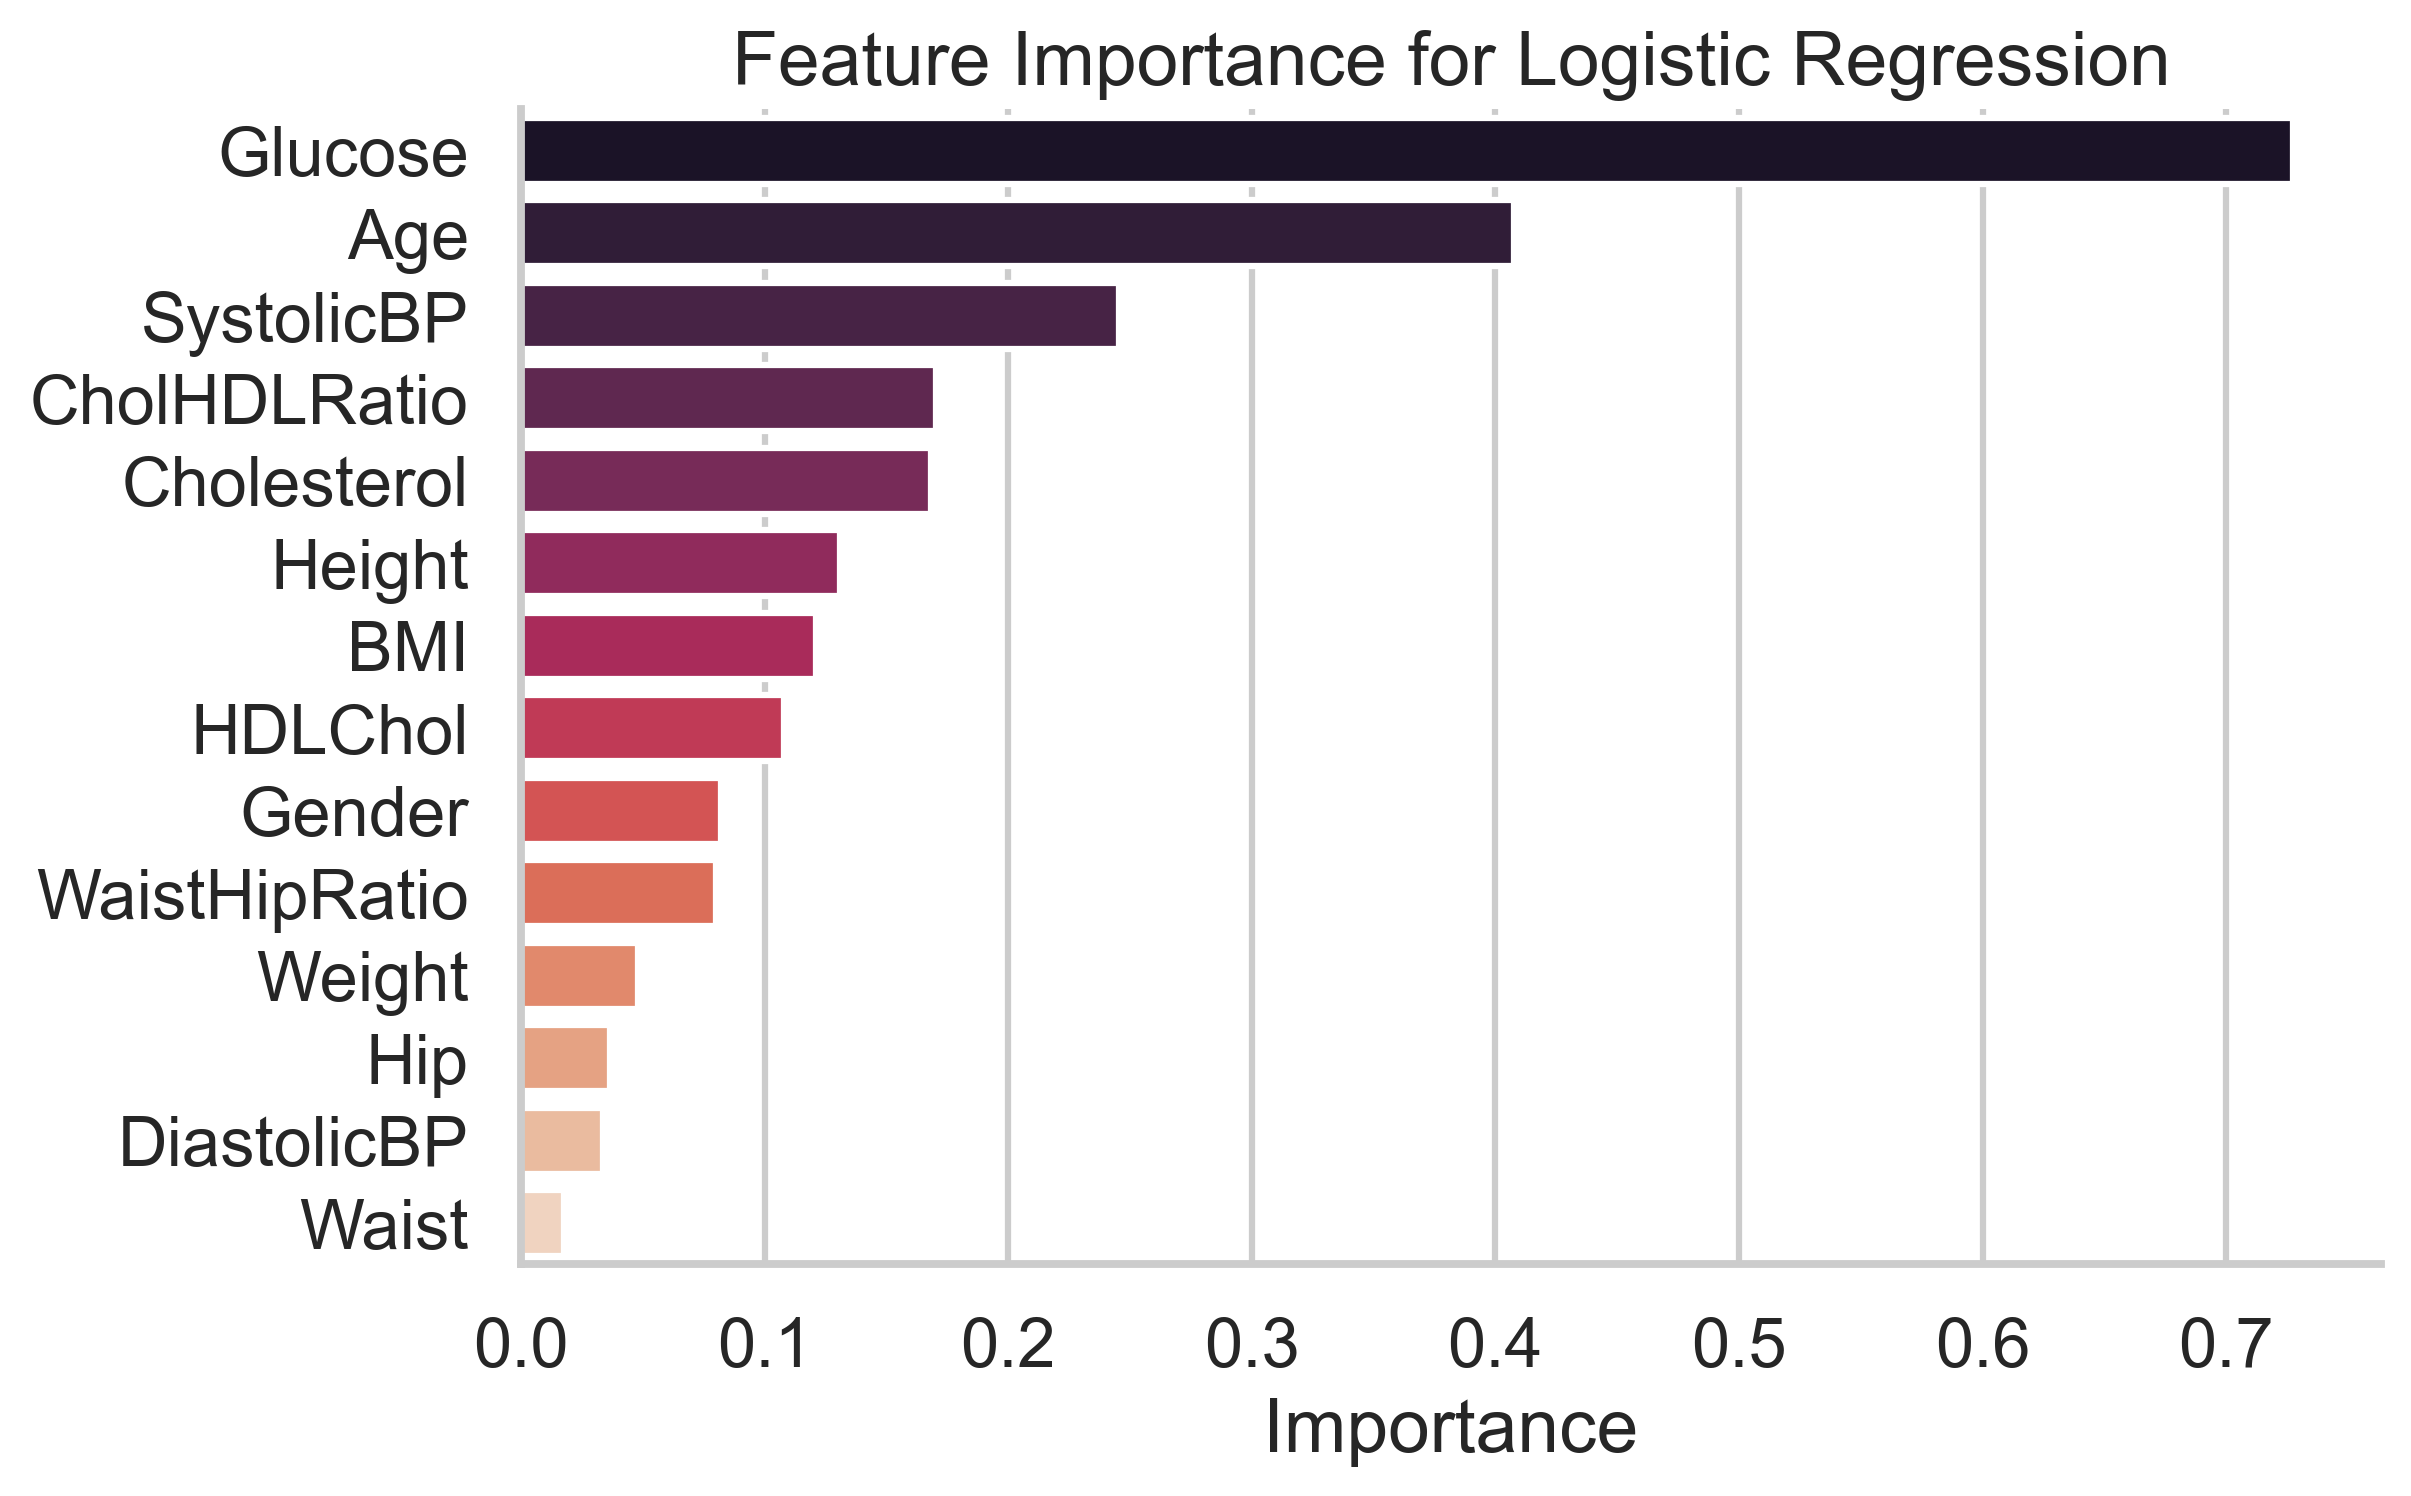
\includegraphics[width=0.78\linewidth]{classification_feature_importance.png}
    \caption{Model-native feature importance summary for the selected Logistic Regression classifier.}
    \label{fig:classification-feature-importance}
\end{figure}

\csvtable{paired_model_comparison.csv}{Paired comparison of the top two classification models across repeated cross-validation folds.}{tab:paired-model-comparison}
\csvtable{recommended_threshold.csv}{Recommended operating-point summary for recall-sensitive diabetes screening.}{tab:recommended-threshold}

\subsection{Regression Results}
For continuous Glucose prediction, Linear Regression outperformed the alternative regressors with a held-out RMSE of 48.9414, MAE of 33.6808, and $R^2$ of 0.2471. As shown in Table~\ref{tab:regression-results-main}, Random Forest Regressor and Gradient Boosting Regressor produced slightly larger errors and lower explained variance, indicating that nonlinear structure did not provide a meaningful advantage in this cohort. The residual diagnostics in Fig.~\ref{fig:regression-diagnostics} suggested roughly centered residuals with moderate spread and larger errors at extreme Glucose values, which is consistent with the modest overall $R^2$.

\csvtable{regression_model_comparison.csv}{Held-out regression performance for the continuous Glucose estimation task.}{tab:regression-results-main}

\begin{figure}[!t]
    \centering
    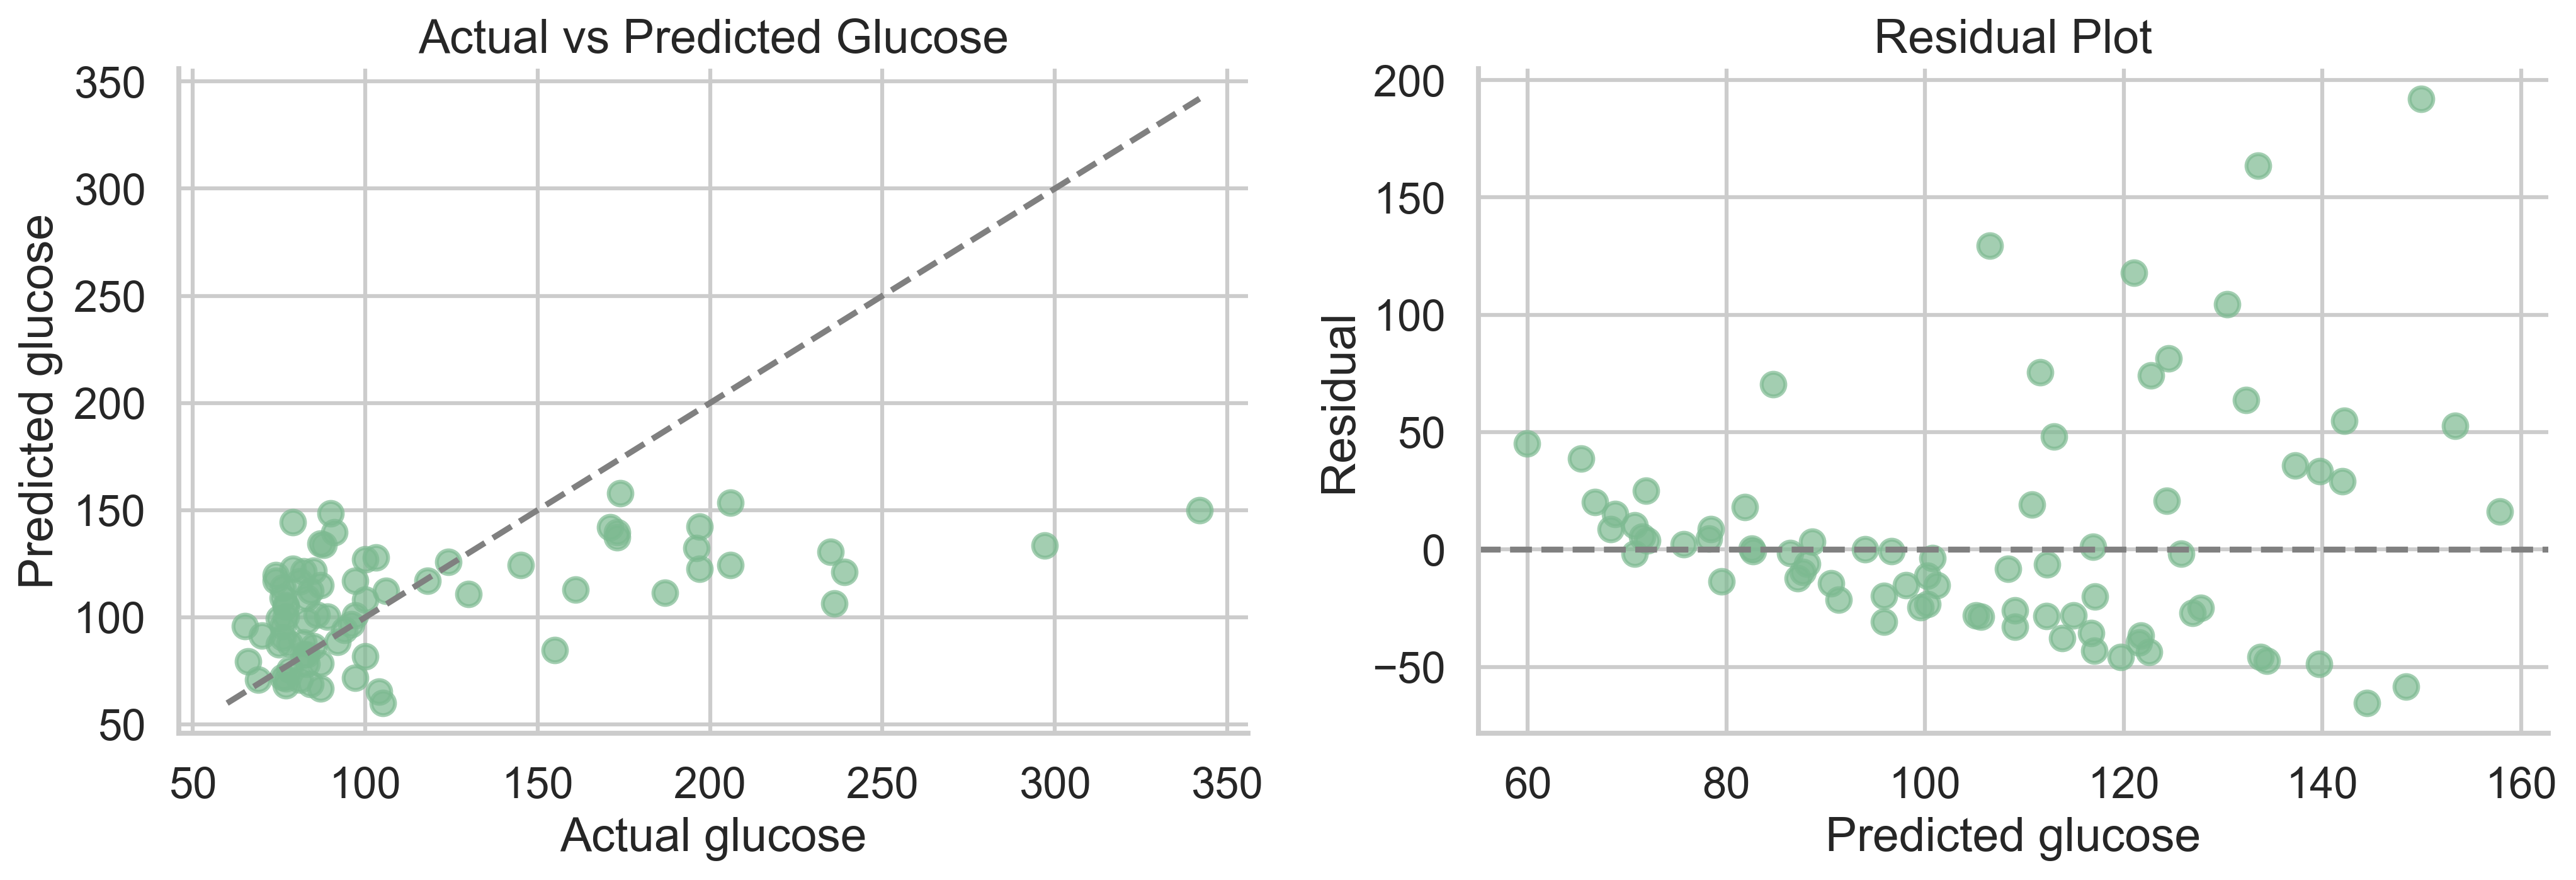
\includegraphics[width=0.9\linewidth]{regression_diagnostics.png}
    \caption{Regression diagnostics showing actual-versus-predicted Glucose values and residual behavior for the compared models.}
    \label{fig:regression-diagnostics}
\end{figure}

\subsection{Clustering Results}
The clustering workflow selected $k=2$ as the most defensible solution. Figure~\ref{fig:clustering-diagnostics} shows that the two-cluster configuration achieved the highest silhouette score (0.4446), whereas solutions with $k=3$ to $k=6$ produced substantially weaker separation. The resulting clusters were clinically interpretable rather than purely mathematical partitions.

Cluster 0 represented a higher-risk profile characterized by markedly elevated Glucose, older age, slightly higher BMI, and a high OutcomePrevalence of 84.44\%. Cluster 1 represented a lower-risk profile with substantially lower Glucose, younger age, slightly lower BMI, and an OutcomePrevalence of only 6.38\%. These differences, summarized in Table~\ref{tab:cluster-results-main} and visualized in Fig.~\ref{fig:clustering-pca}, indicate that unsupervised learning captured meaningful variation in cardiometabolic burden across the cohort.

\begin{figure}[!t]
    \centering
    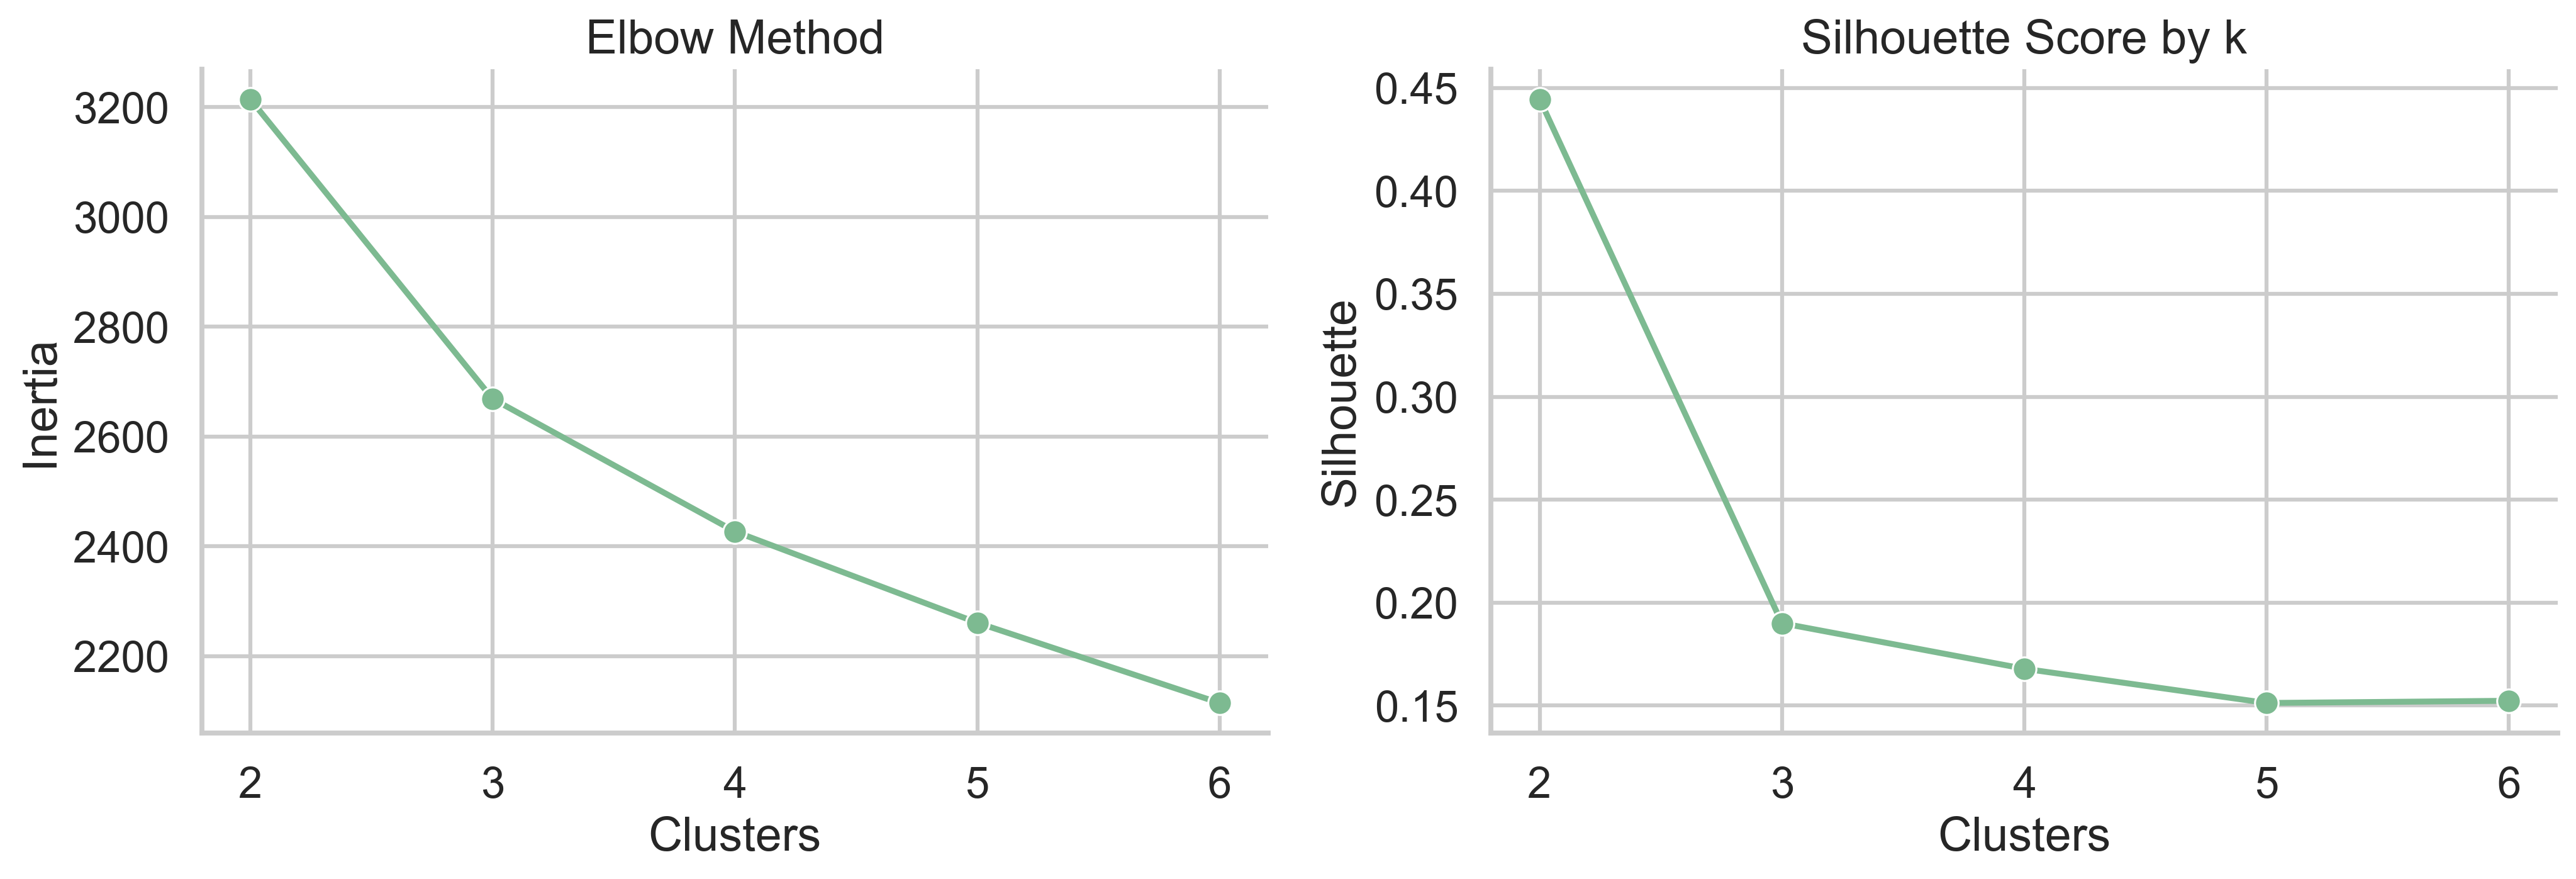
\includegraphics[width=0.84\linewidth]{clustering_diagnostics.png}
    \caption{Elbow and silhouette diagnostics used to support cluster-count selection.}
    \label{fig:clustering-diagnostics}
\end{figure}

\begin{figure}[!t]
    \centering
    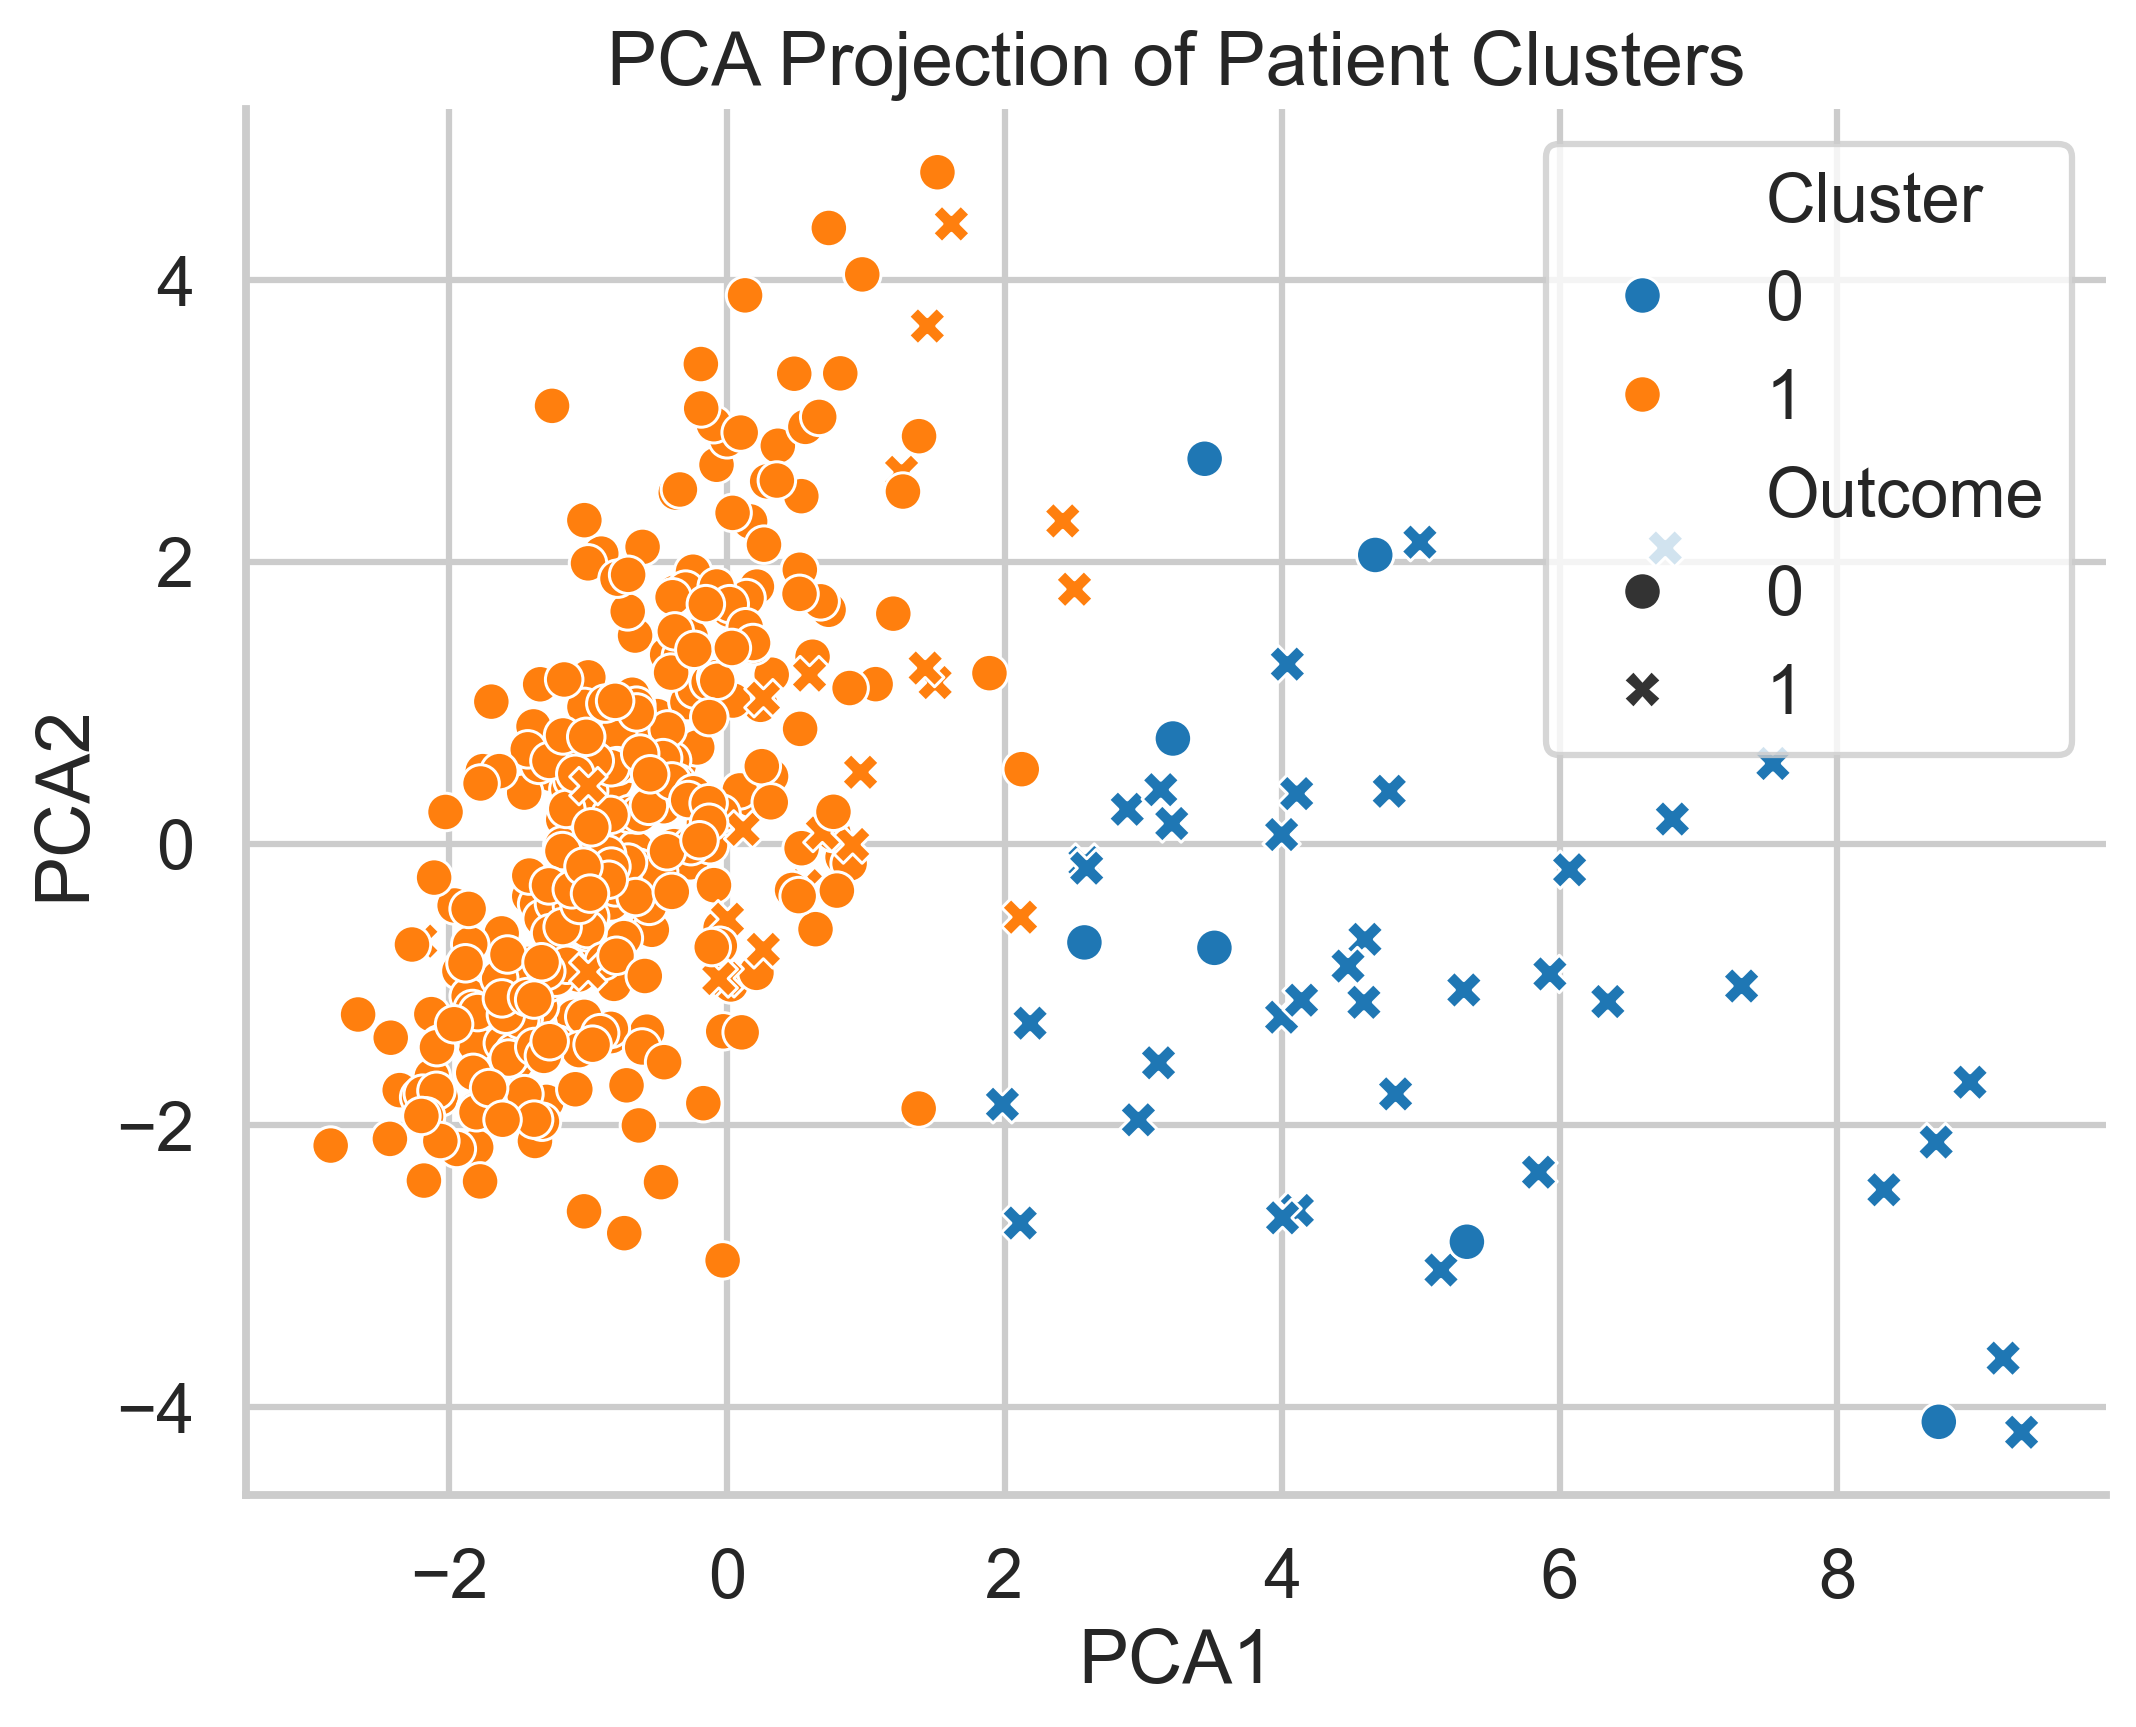
\includegraphics[width=0.84\linewidth]{clustering_pca_projection.png}
    \caption{PCA projection of the selected clustering solution for visual interpretation of patient subgroups.}
    \label{fig:clustering-pca}
\end{figure}

\begin{table*}[!t]
\centering
\caption{Summary of cluster-level cardiometabolic profiles and OutcomePrevalence.}
\label{tab:cluster-results-main}
\footnotesize
\setlength{\tabcolsep}{5pt}
\renewcommand{\arraystretch}{1.1}
\begin{tabular}{c c c c c c p{6.0cm}}
\toprule
Cluster & Count & OutcomePrevalence & Glucose & BMI & Age & Cluster Label \\
\midrule
0 & 45 & 84.44\% & 237.33 & 30.51 & 58.98 & Higher-Risk Older Hyperglycemic Profile \\
1 & 345 & 6.38\% & 90.38 & 28.55 & 45.18 & Lower-Risk Younger Normoglycemic Profile \\
\bottomrule
\end{tabular}
\end{table*}

\subsection{Explainability Results}
Explainability analysis consistently identified Glucose, Age, and SystolicBP as the dominant contributors to predicted diabetes risk. At the global level, the SHAP summaries in Figs.~\ref{fig:shap-beeswarm} and~\ref{fig:shap-bar} indicated that higher Glucose, older age, higher SystolicBP, and less favorable lipid measures such as CholHDLRatio increased predicted risk, whereas more favorable HDLChol values reduced it. This use of SHAP is consistent with broader explainable-AI practice in healthcare, where global and local explanations are used to improve transparency and interpretability \cite{xai_healthcare,xai_shap,xai_ehr}. The model-native importance ranking showed the same overall pattern, with Cholesterol and CholHDLRatio also contributing meaningfully after the top three predictors.

At the patient level, the local SHAP explanation illustrated how elevated SystolicBP, older age, and adverse lipid markers combined to increase risk for an illustrative high-risk case. Together, the global and local explanations improved the transparency of the predictive pipeline and provided clinically plausible rationales for the model output.

\begin{figure}[!t]
    \centering
    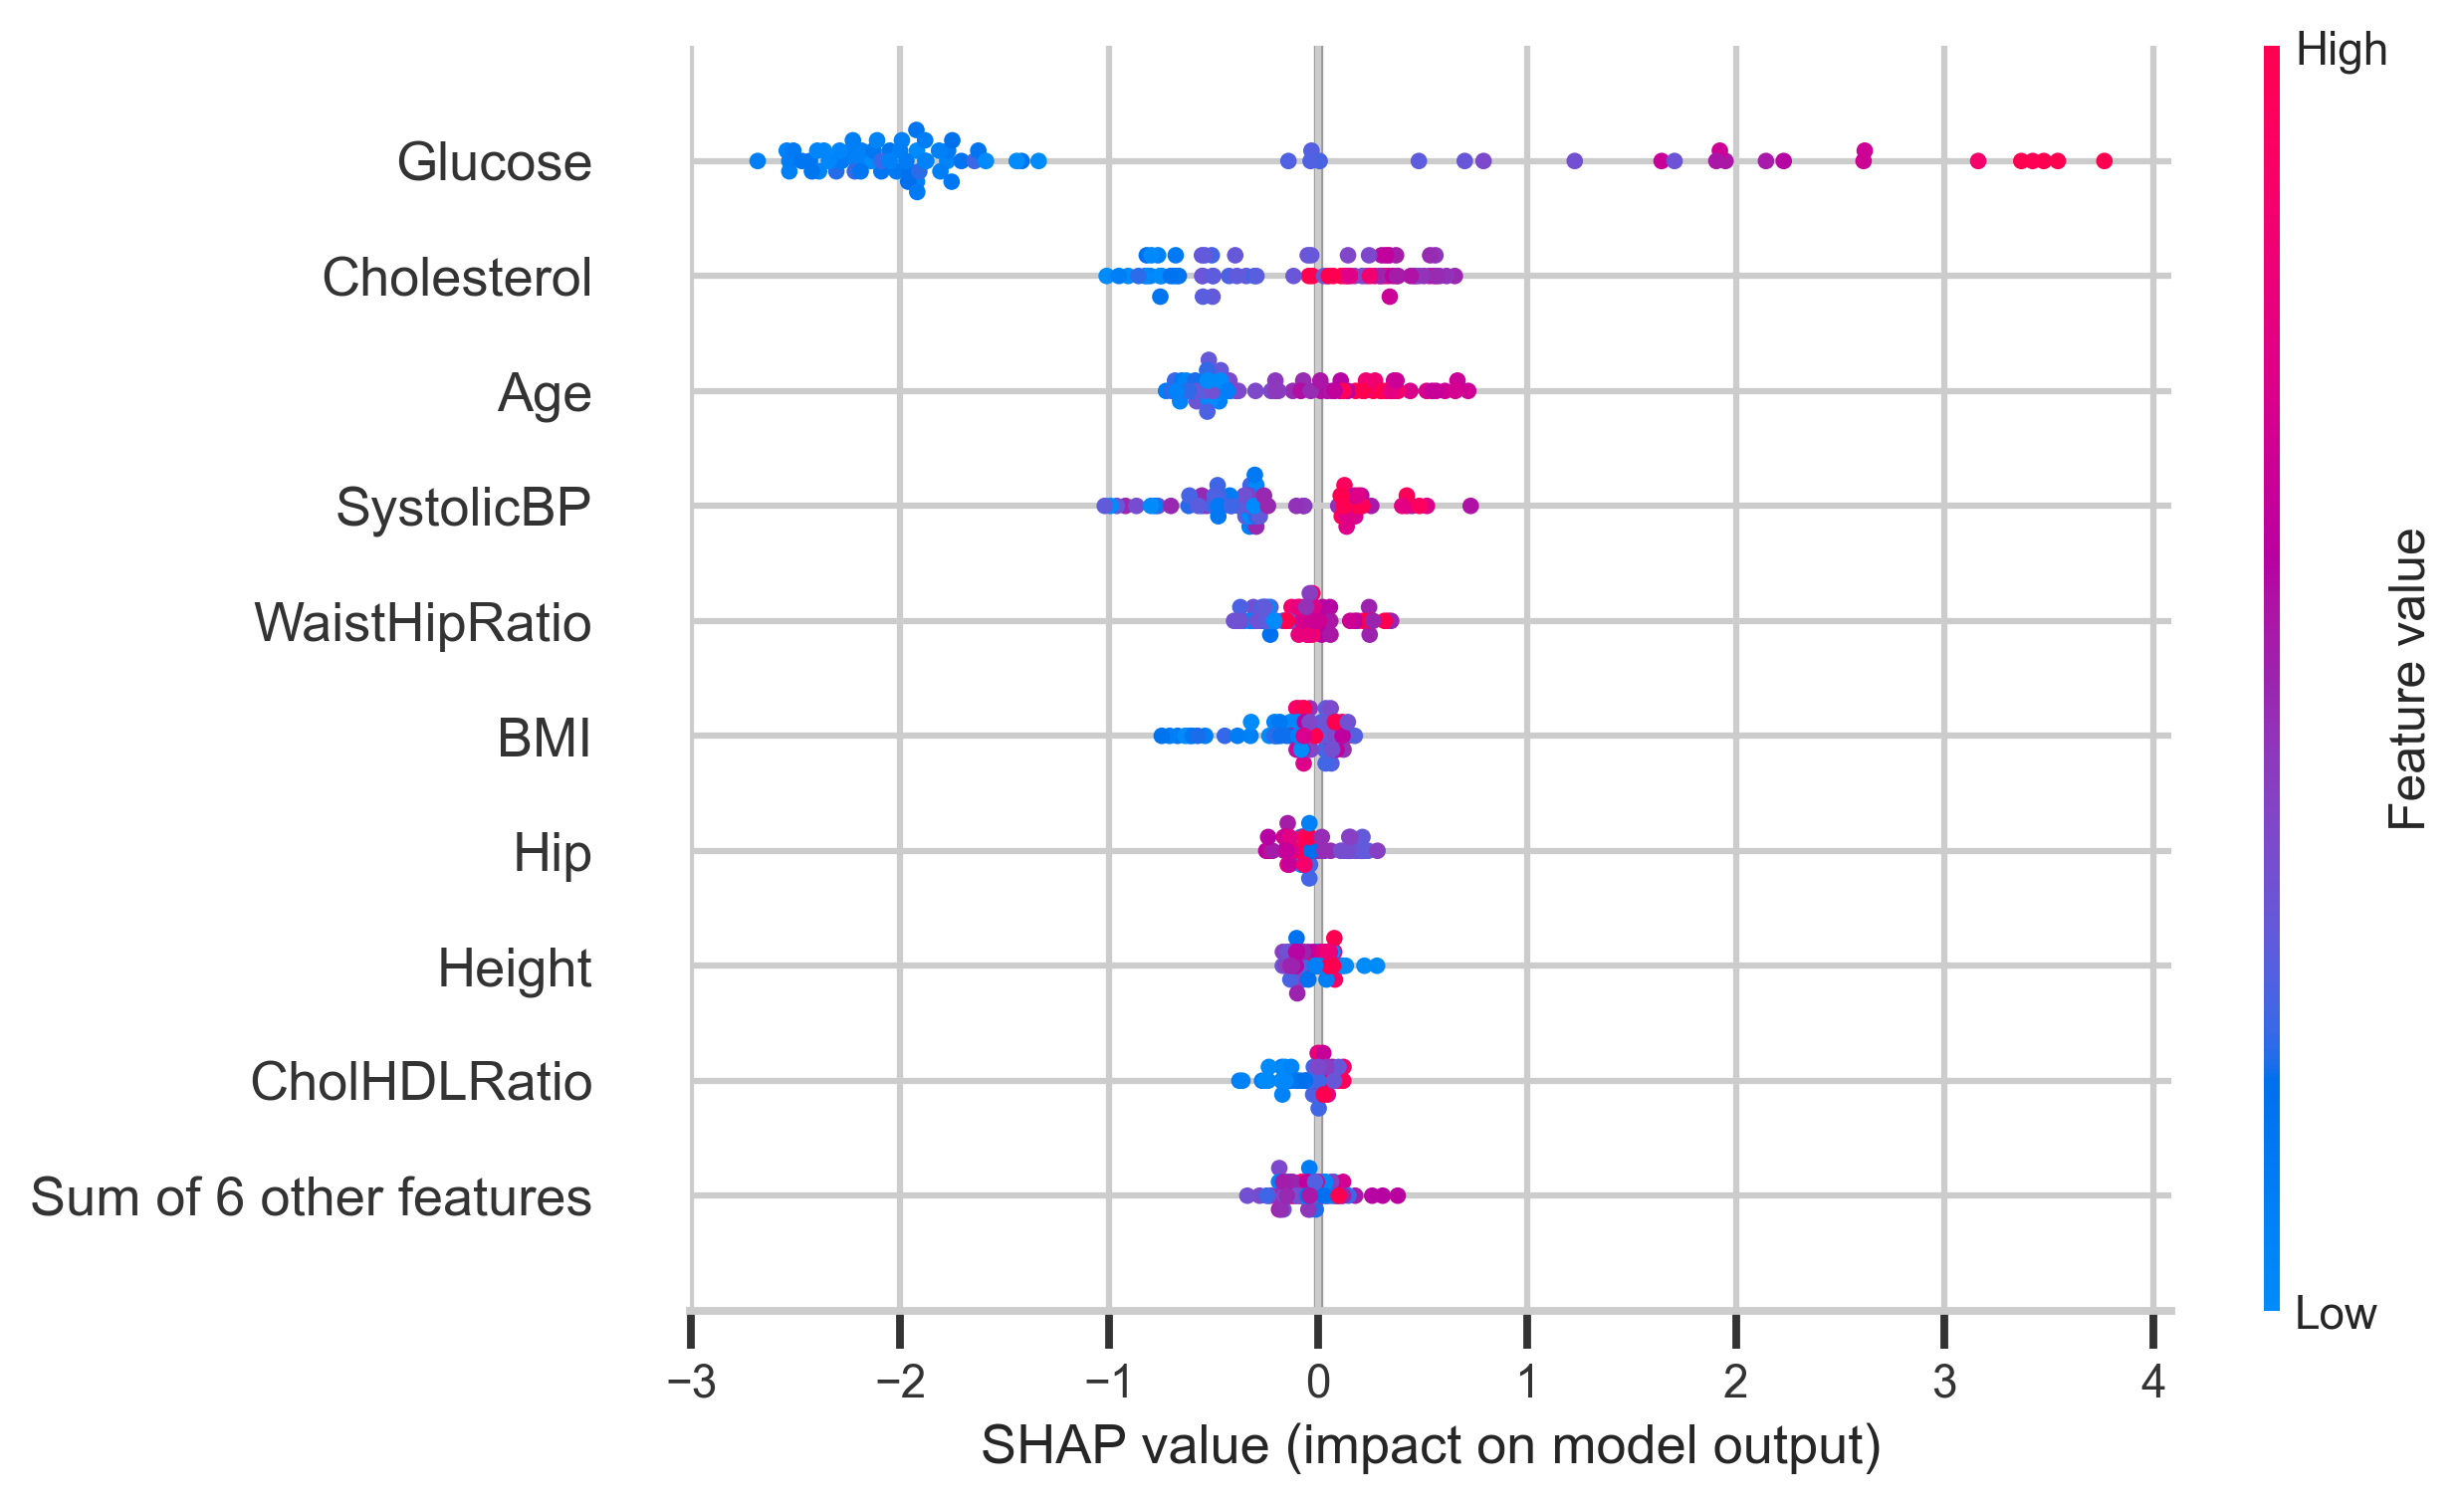
\includegraphics[width=0.92\linewidth]{shap_beeswarm.png}
    \caption{Global SHAP beeswarm plot summarizing both feature importance and directional contribution to predicted diabetes risk.}
    \label{fig:shap-beeswarm}
\end{figure}

\begin{figure}[!t]
    \centering
    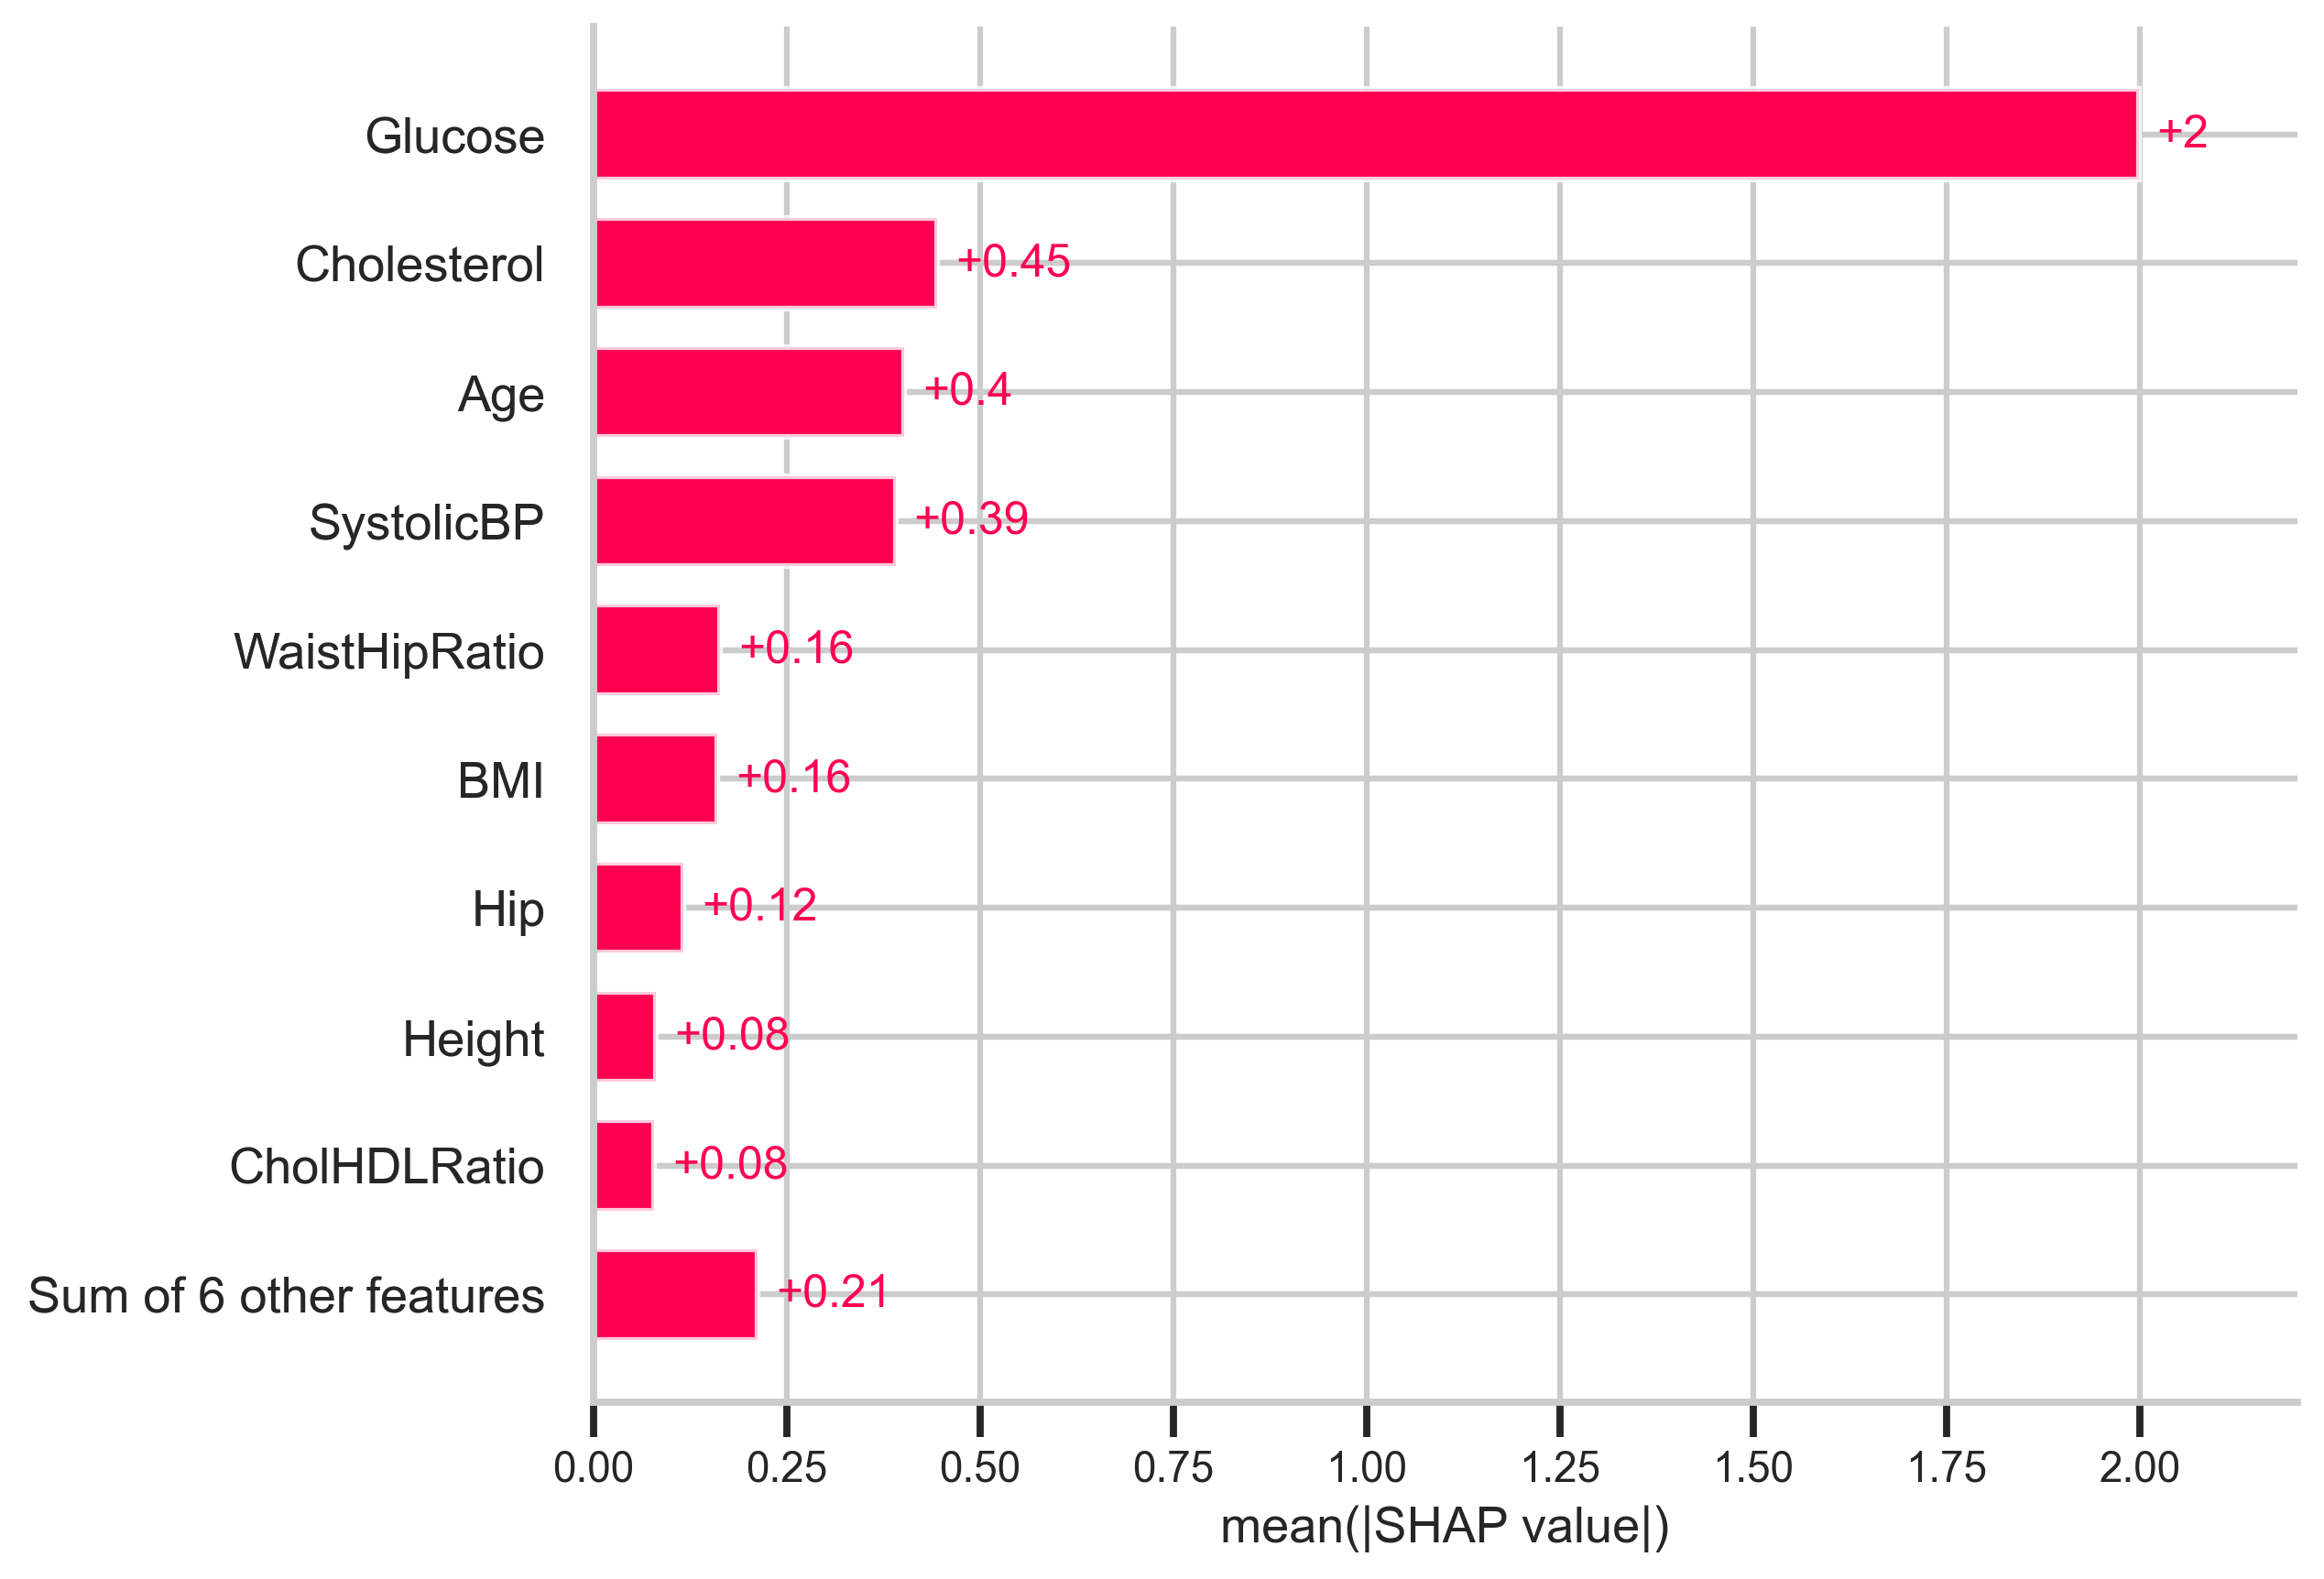
\includegraphics[width=0.75\linewidth]{shap_bar_importance.png}
    \caption{Ranked SHAP importance values for the most influential predictors in the selected classification model.}
    \label{fig:shap-bar}
\end{figure}

\section{Discussion}
This study shows that a multi-task healthcare analytics workflow can yield richer insight than a single-model benchmark. The classification results demonstrate that Logistic Regression provided the strongest held-out ROC-AUC and good calibration, while Support Vector Machine offered the better recall-sensitive operating point with fewer false negatives at the default threshold. When combined with threshold tuning, these findings suggest that operating-point selection may be as important as model-family selection in recall-sensitive diabetes screening settings \cite{ml_diabetes1,ml_diabetes2,calibration}.

The regression results add a complementary perspective. Although Linear Regression achieved the best performance for continuous Glucose estimation, the modest $R^2$ indicates that the available predictors do not fully explain glycemic variation in this dataset. In practical terms, the regression model is better interpreted as a supportive analytics tool than as a substitute for direct biochemical measurement, which is consistent with the broader caution in diabetes prediction studies against over-interpreting performance from small structured cohorts \cite{ml_diabetes3}.

The clustering results reinforce the value of stratified analysis. Two distinct patient subgroups emerged: a higher-risk, older, hyperglycemic cluster with very high OutcomePrevalence and a lower-risk, younger cluster with substantially lower metabolic burden. This unsupervised separation complements the supervised findings by showing that the cohort contains clinically meaningful heterogeneity rather than a single homogeneous risk distribution \cite{cluster_diabetes}.

The explainability findings strengthen the clinical plausibility of the overall workflow. Glucose, Age, and SystolicBP consistently emerged as the most influential predictors across model-native and SHAP-based explanations, while lipid measures provided additional context. This convergence is important because it links the classification findings, the cluster profiles, and the practical implications of the study through a shared set of clinically recognizable risk factors \cite{xai_healthcare,xai_shap,xai_ehr}.

\section{Practical Implications}
The developed workflow has several realistic healthcare applications. In hospital screening pathways, it could support triage by identifying patients who merit confirmatory testing or earlier metabolic assessment. In community or mobile-health settings, it could provide preliminary risk stratification and guide follow-up recommendations. Because threshold tuning delivered a zero-false-negative operating point in the held-out sample, the workflow is particularly well aligned with settings in which missed high-risk patients are more costly than additional confirmatory tests.

The cluster-based findings also have operational value because they can be translated into subgroup-specific intervention strategies. Patients resembling the higher-risk cluster may warrant closer outreach, metabolic monitoring, and lifestyle counseling, whereas the lower-risk cluster may be more appropriate for lighter-touch prevention programs. Explainability outputs further help translate model predictions into clinician-facing and patient-facing narratives that are easier to audit and discuss.

\section{Limitations}
This study has several limitations. First, the dataset is relatively small, which limits statistical power and increases the risk of unstable performance estimates. Second, the cohort source and demographic structure may not generalize to broader populations or to other healthcare environments. Third, the feature set is restricted to structured diagnostic and anthropometric measures and does not include medication use, prior laboratory history, comorbidities, lifestyle factors, social determinants of health, or longitudinal follow-up.

Methodologically, the analysis is based on a single tabular dataset, so the findings should be interpreted as internally valid but preliminary. Even a well-performing model in this study would still require external validation, subgroup fairness assessment, calibration monitoring, and governance review before real-world deployment. Finally, explainability methods such as SHAP improve transparency but do not establish causality; they should therefore be interpreted as descriptive rather than causal evidence.

\section{Conclusion}
This mini research project demonstrates how classification, regression, clustering, and explainability can be integrated into a coherent healthcare analytics workflow for diabetes risk stratification. Logistic Regression achieved the strongest held-out ROC-AUC, while Support Vector Machine offered the most recall-sensitive default operating point with fewer false negatives. Linear Regression provided the most accurate continuous Glucose estimates, and Glucose, Age, and SystolicBP were the most influential predictors of modeled risk. The clustering analysis additionally revealed a clear separation between a higher-risk older hyperglycemic subgroup and a lower-risk younger subgroup with much lower OutcomePrevalence.

Overall, the study supports the view that explainable, multi-task machine learning can provide richer clinical insight than a single-task benchmark alone. With larger and more representative data, similar workflows could contribute to scalable screening, stratified prevention, and better-informed personalized intervention planning.

\begin{thebibliography}{00}

\bibitem{dataset}
H. Benmansour, ``Predict diabetes based on diagnostic measures,'' Kaggle dataset, 2020. [Online]. Available: \url{https://www.kaggle.com/datasets/houcembenmansour/predict-diabetes-based-on-diagnostic-measures}. [Accessed: Apr. 22, 2026].

\bibitem{ml_diabetes1}
S. Perveen, M. Shahbaz, A. Guergachi, and K. Keshavjee, ``Performance analysis of data mining classification techniques to predict diabetes,'' \textit{Procedia Computer Science}, vol. 82, pp. 115--121, 2016.

\bibitem{ml_diabetes2}
H. Lai, H. Huang, K. Keshavjee, A. Guergachi, and X. Gao, ``Predictive models for diabetes mellitus using machine learning techniques,'' \textit{BMC Endocrine Disorders}, vol. 19, no. 1, Art. no. 101, 2019.

\bibitem{ml_diabetes3}
I. Kavakiotis, O. Tsave, A. Salifoglou, N. Maglaveras, I. Vlahavas, and I. Chouvarda, ``Machine learning and data mining methods in diabetes research,'' \textit{Computational and Structural Biotechnology Journal}, vol. 15, pp. 104--116, 2017.

\bibitem{calibration}
B. Van Calster, D. J. McLernon, M. van Smeden, L. Wynants, and E. W. Steyerberg, ``Calibration: The Achilles heel of predictive analytics,'' \textit{BMC Medicine}, vol. 17, Art. no. 230, 2019.

\bibitem{steyerberg2019}
E. W. Steyerberg, \textit{Clinical Prediction Models}, 2nd ed. Cham, Switzerland: Springer, 2019.

\bibitem{cluster_diabetes}
E. Ahlqvist \textit{et al.}, ``Novel subgroups of adult-onset diabetes and their association with outcomes: A data-driven cluster analysis of six variables,'' \textit{The Lancet Diabetes \& Endocrinology}, vol. 6, no. 5, pp. 361--369, 2018.

\bibitem{xai_healthcare}
A. Holzinger, C. Biemann, C. S. Pattichis, and D. B. Kell, ``What do we need to build explainable AI systems for the medical domain?,'' \textit{arXiv preprint arXiv:1712.09923}, 2017.

\bibitem{xai_shap}
S. M. Lundberg and S.-I. Lee, ``A unified approach to interpreting model predictions,'' in \textit{Advances in Neural Information Processing Systems 30}, 2017, pp. 4765--4774.

\bibitem{xai_ehr}
S. M. Lauritsen \textit{et al.}, ``Explainable artificial intelligence model to predict acute critical illness from electronic health records,'' \textit{Nature Communications}, vol. 11, Art. no. 3852, 2020.

\end{thebibliography}

\clearpage
\appendices

\section{Reproducibility Setup}
\begin{itemize}[leftmargin=1.5em]
    \item Python environment: Python 3.12 with pandas 3.0.2, numpy 2.4.4, seaborn 0.13.2, scikit-learn 1.8.0, xgboost 3.2.0, and shap 0.51.0.
    \item Random seed: 42
\end{itemize}

\csvtable{package_versions.csv}{Package versions used to support reproducibility of the notebook results.}{tab:package-versions}

\section{Supplementary Figures}

\begin{figure}[!t]
    \centering
    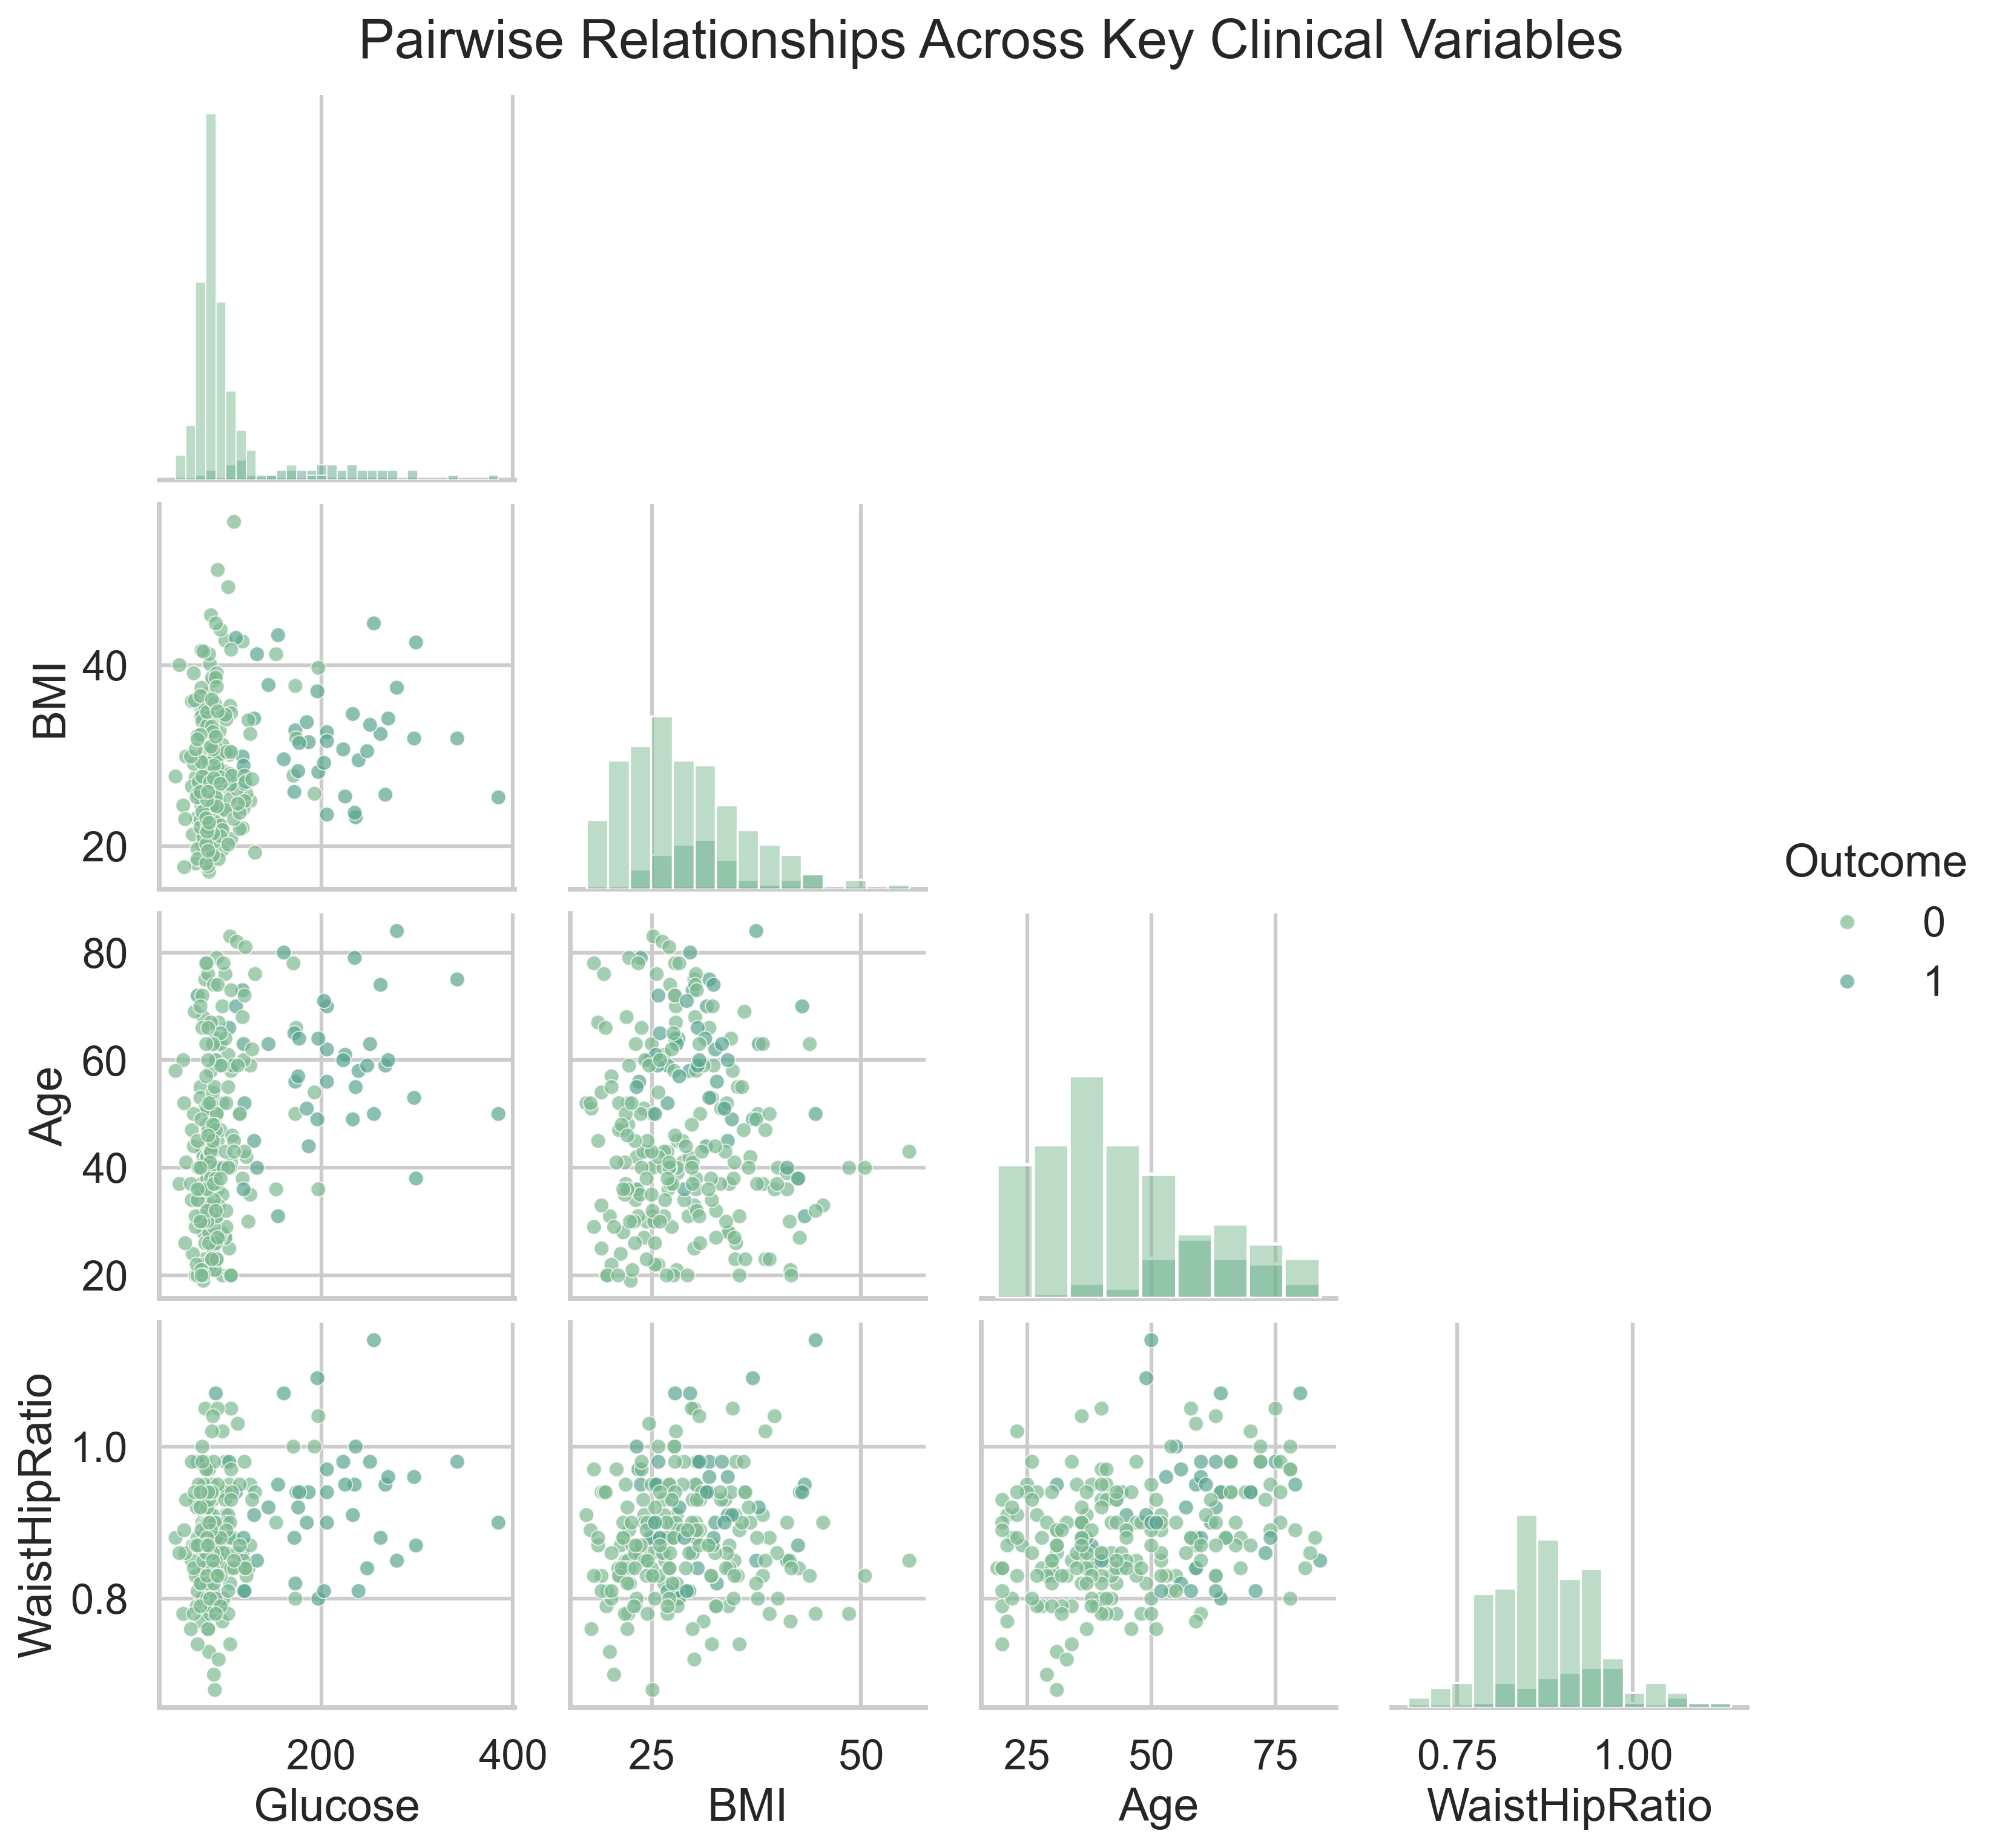
\includegraphics[width=0.88\linewidth]{pairplot_key_features.png}
    \caption{Appendix pairplot for a focused subset of key predictors used in exploratory analysis.}
    \label{fig:pairplot-key-features}
\end{figure}

\begin{figure}[!t]
    \centering
    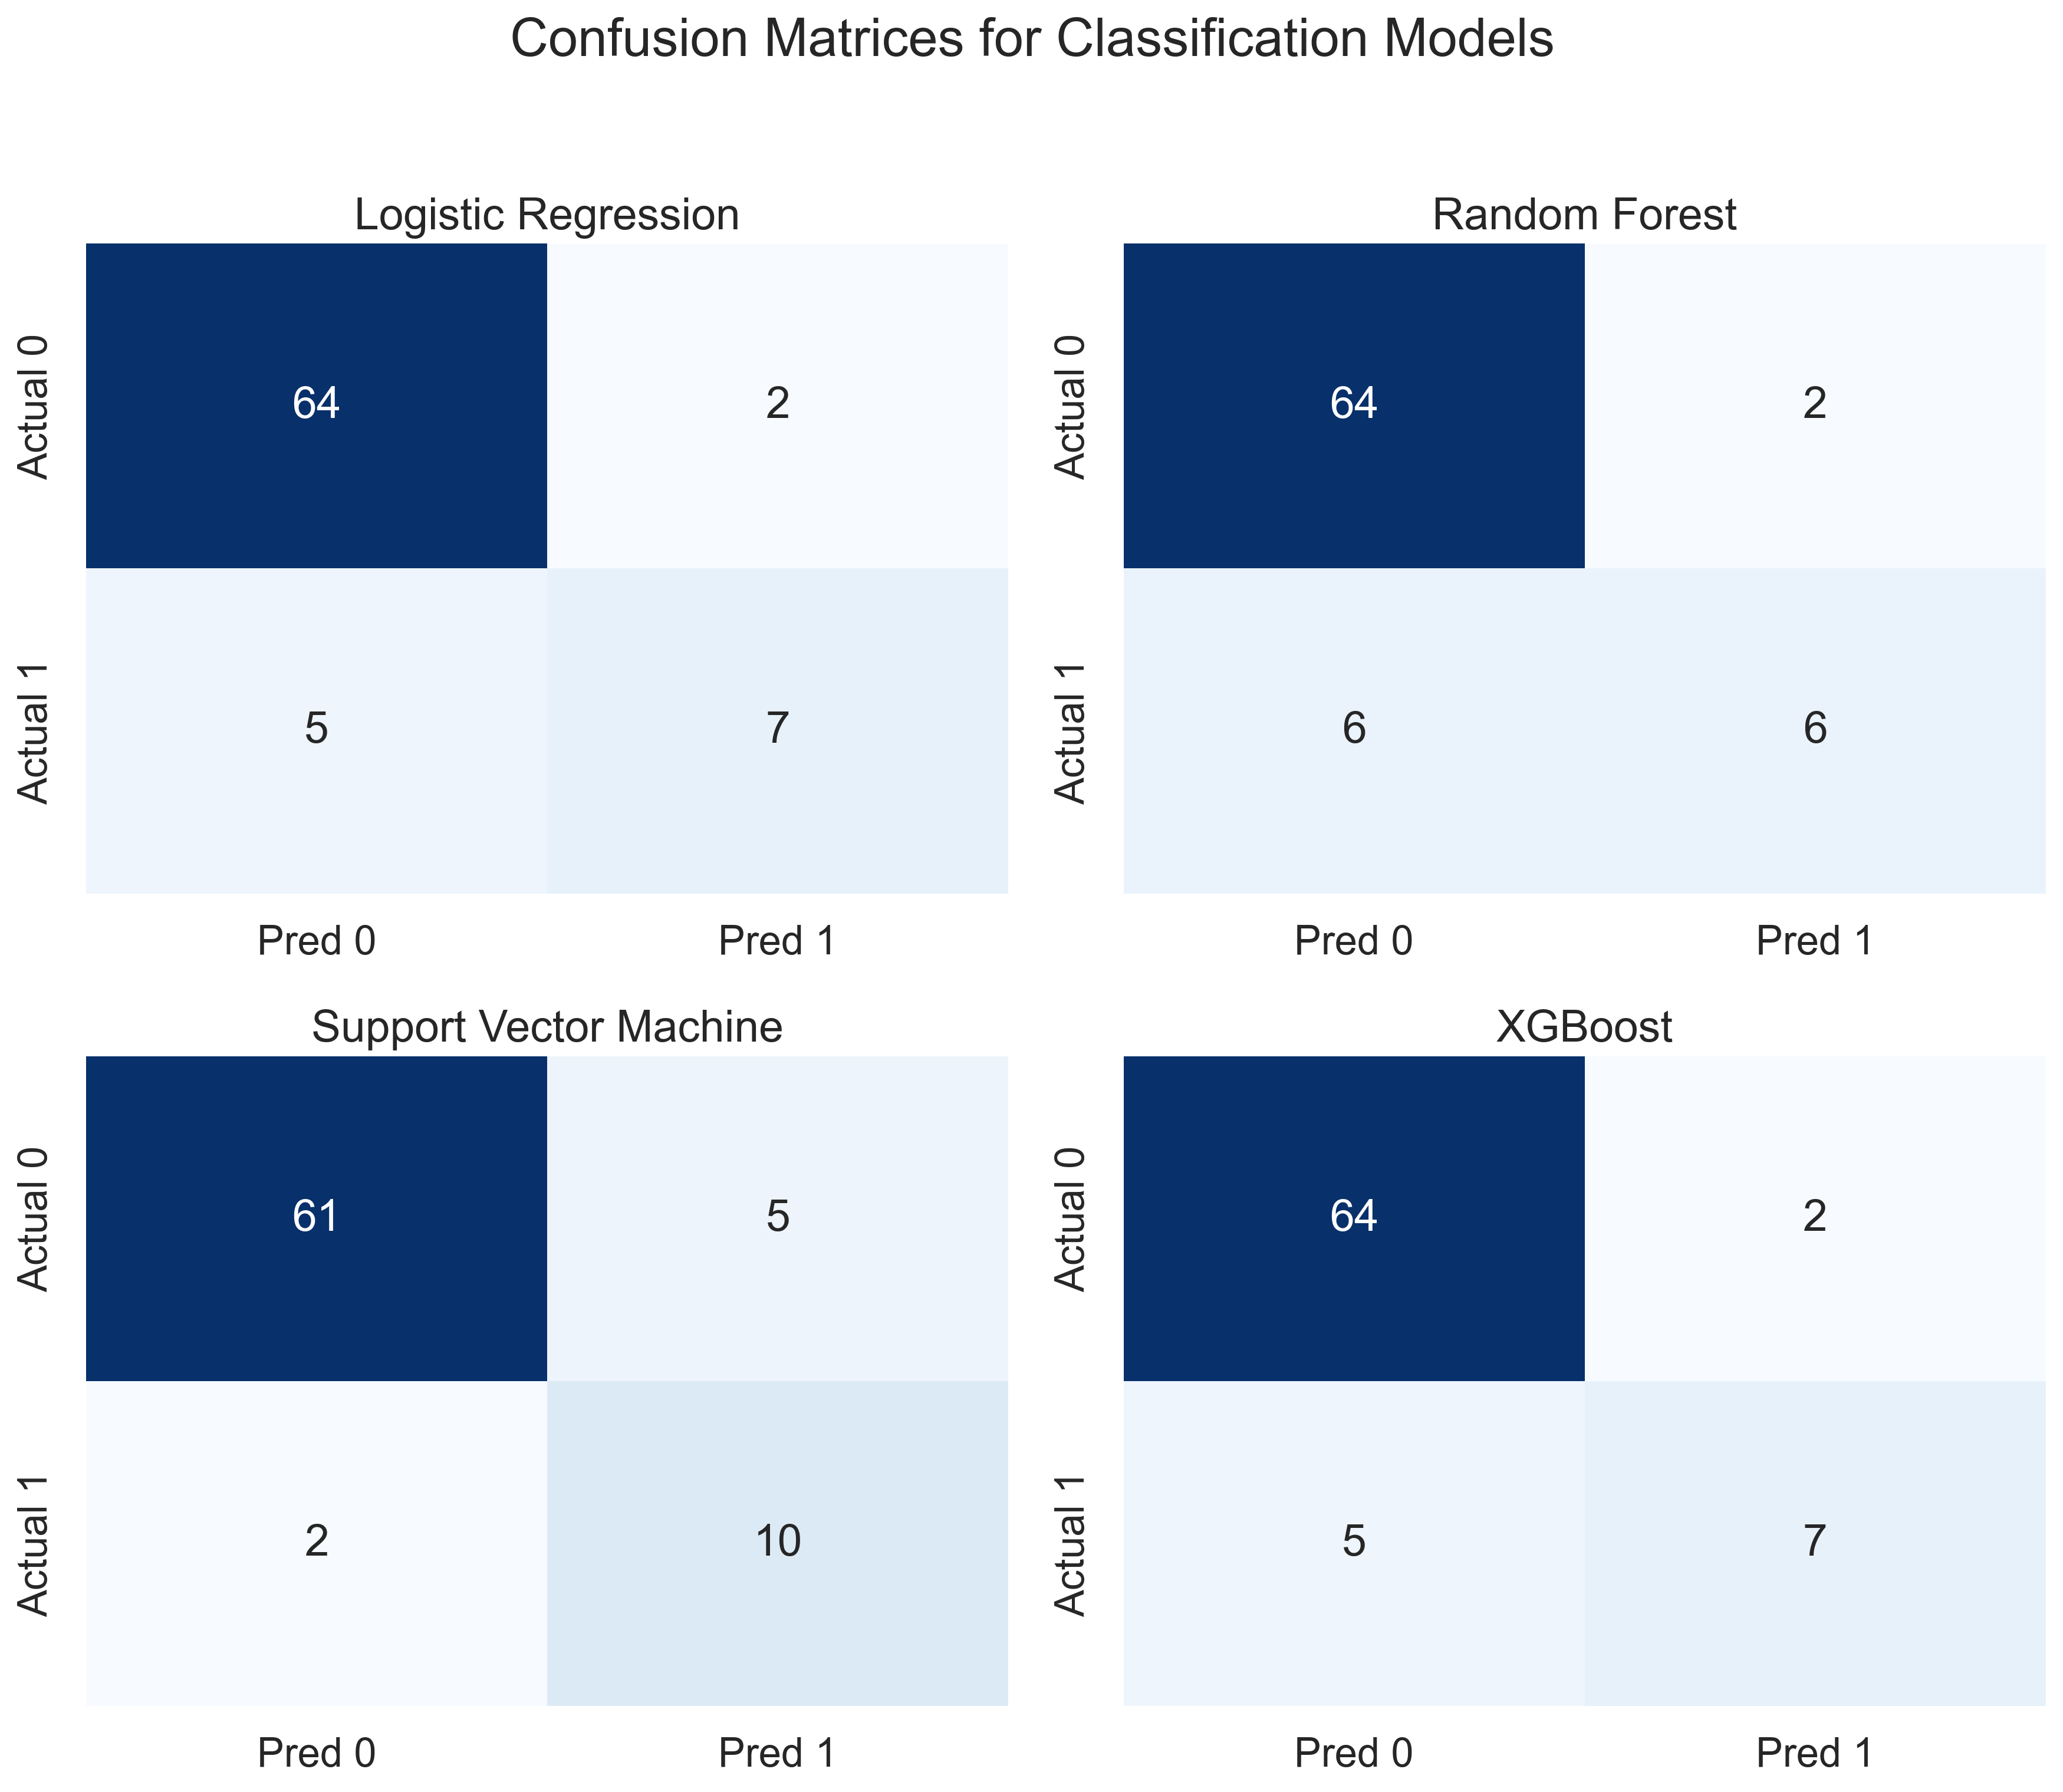
\includegraphics[width=0.86\linewidth]{classification_confusion_matrices.png}
    \caption{Appendix confusion matrices for the compared classification models.}
    \label{fig:appendix-confusion}
\end{figure}

\begin{figure}[!t]
    \centering
    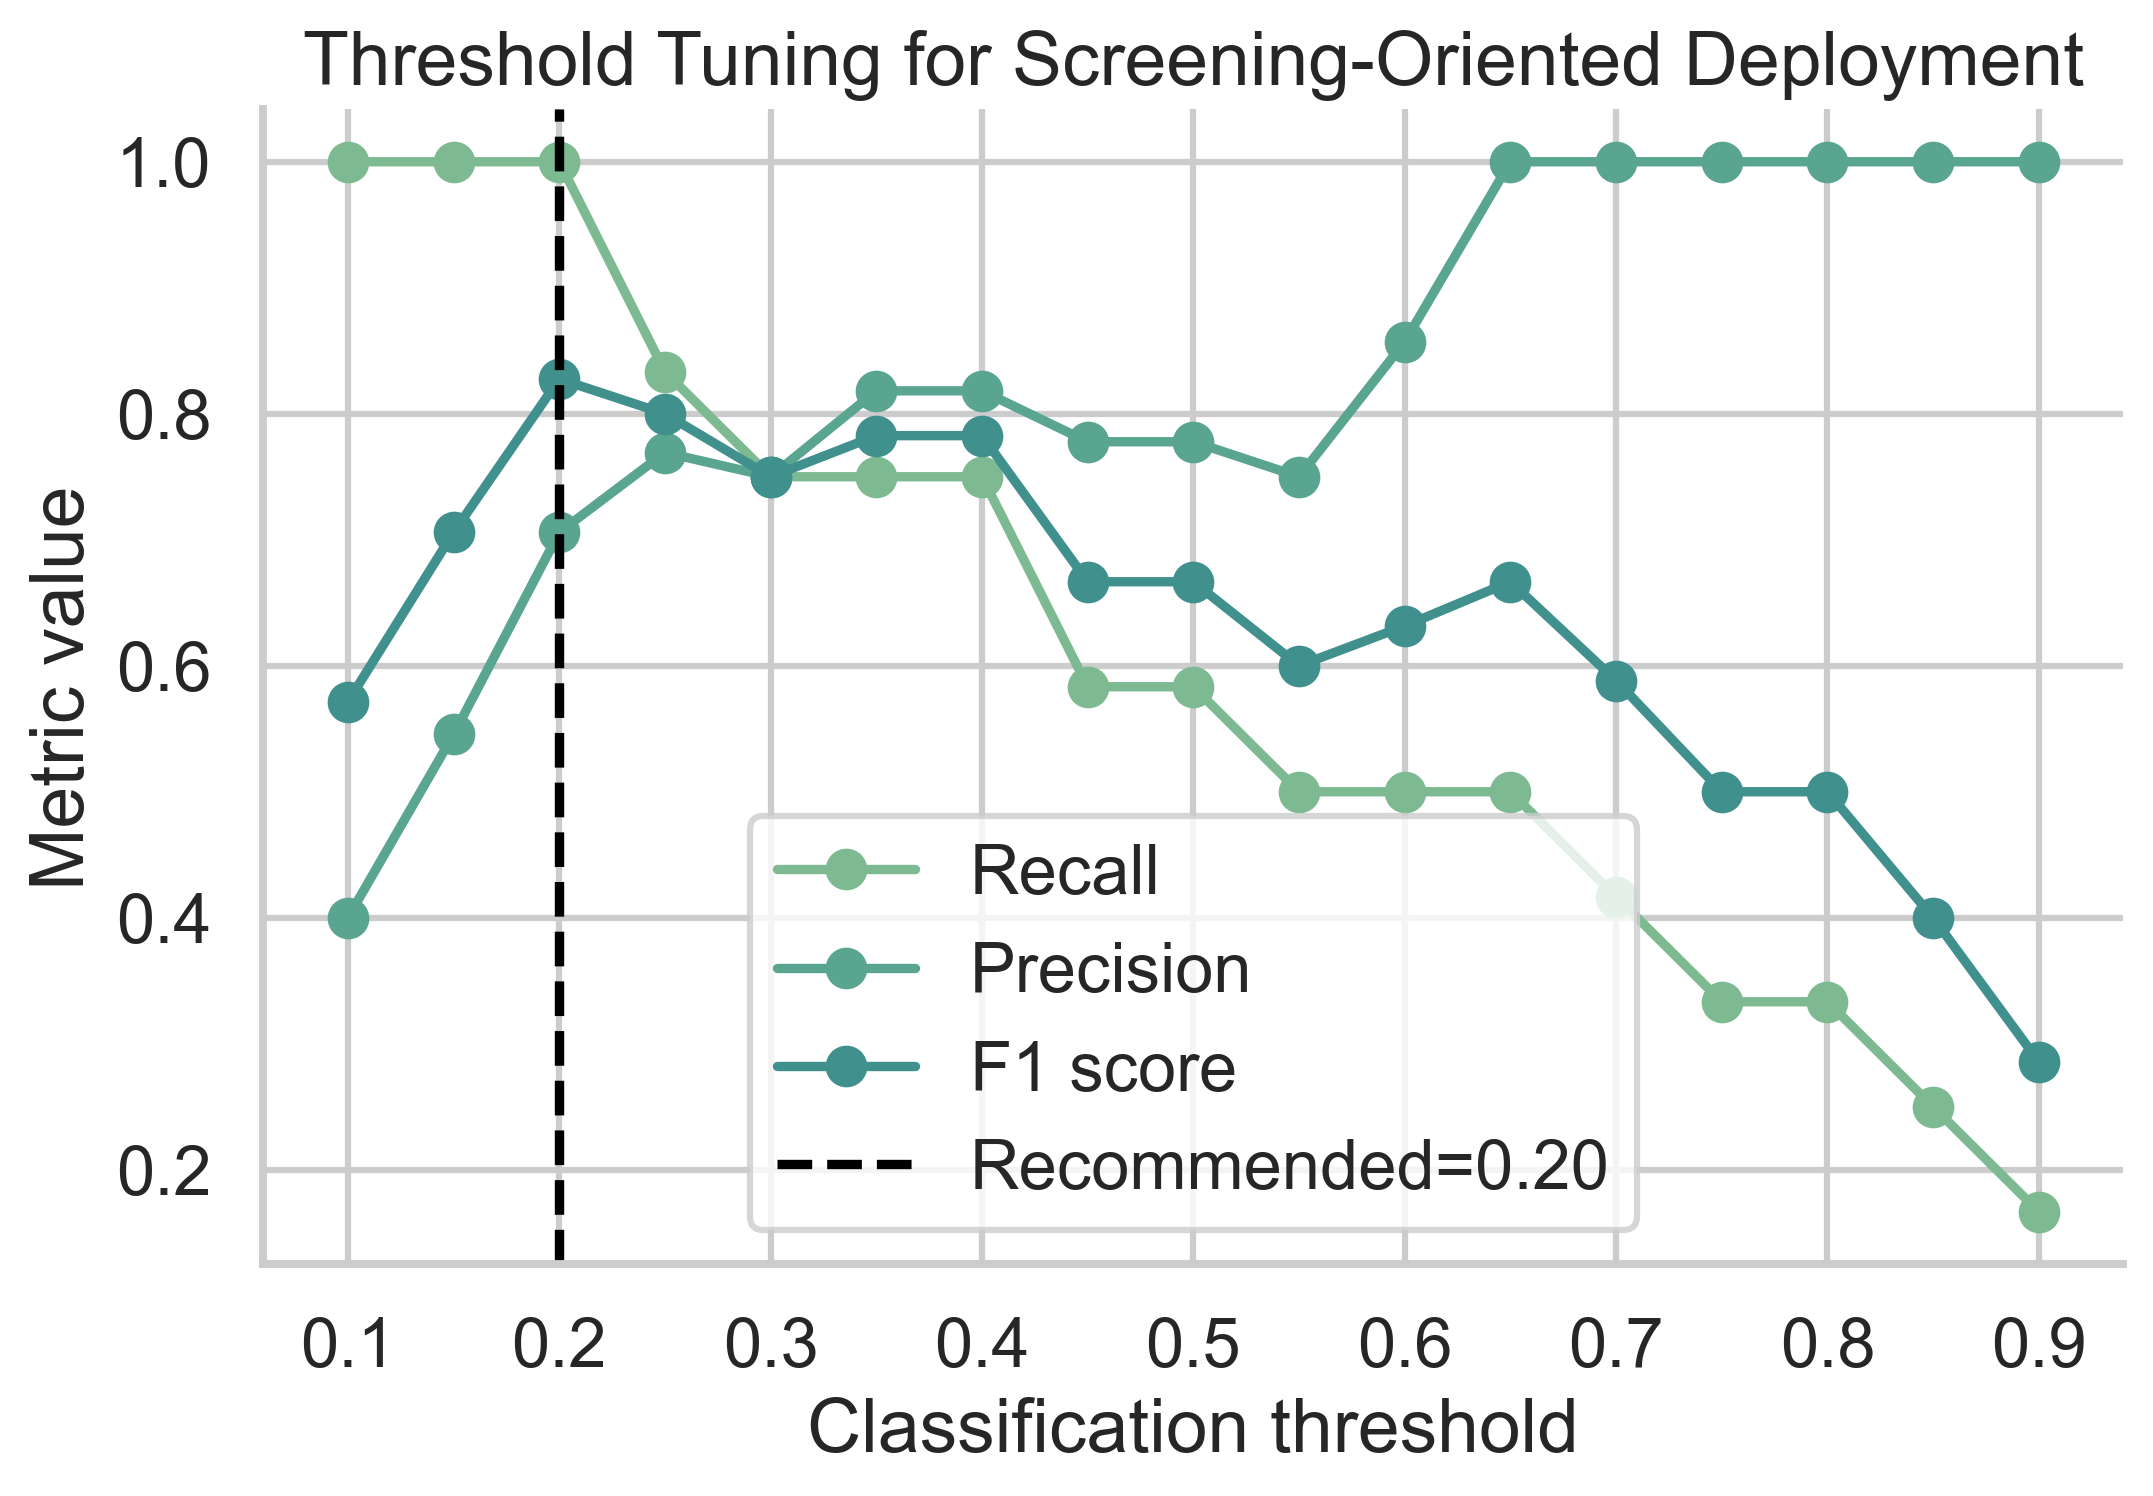
\includegraphics[width=0.84\linewidth]{classification_threshold_sweep.png}
    \caption{Appendix threshold sweep for the selected classifier, illustrating precision-recall trade-offs under alternative decision thresholds.}
    \label{fig:appendix-threshold}
\end{figure}

\begin{figure}[!t]
    \centering
    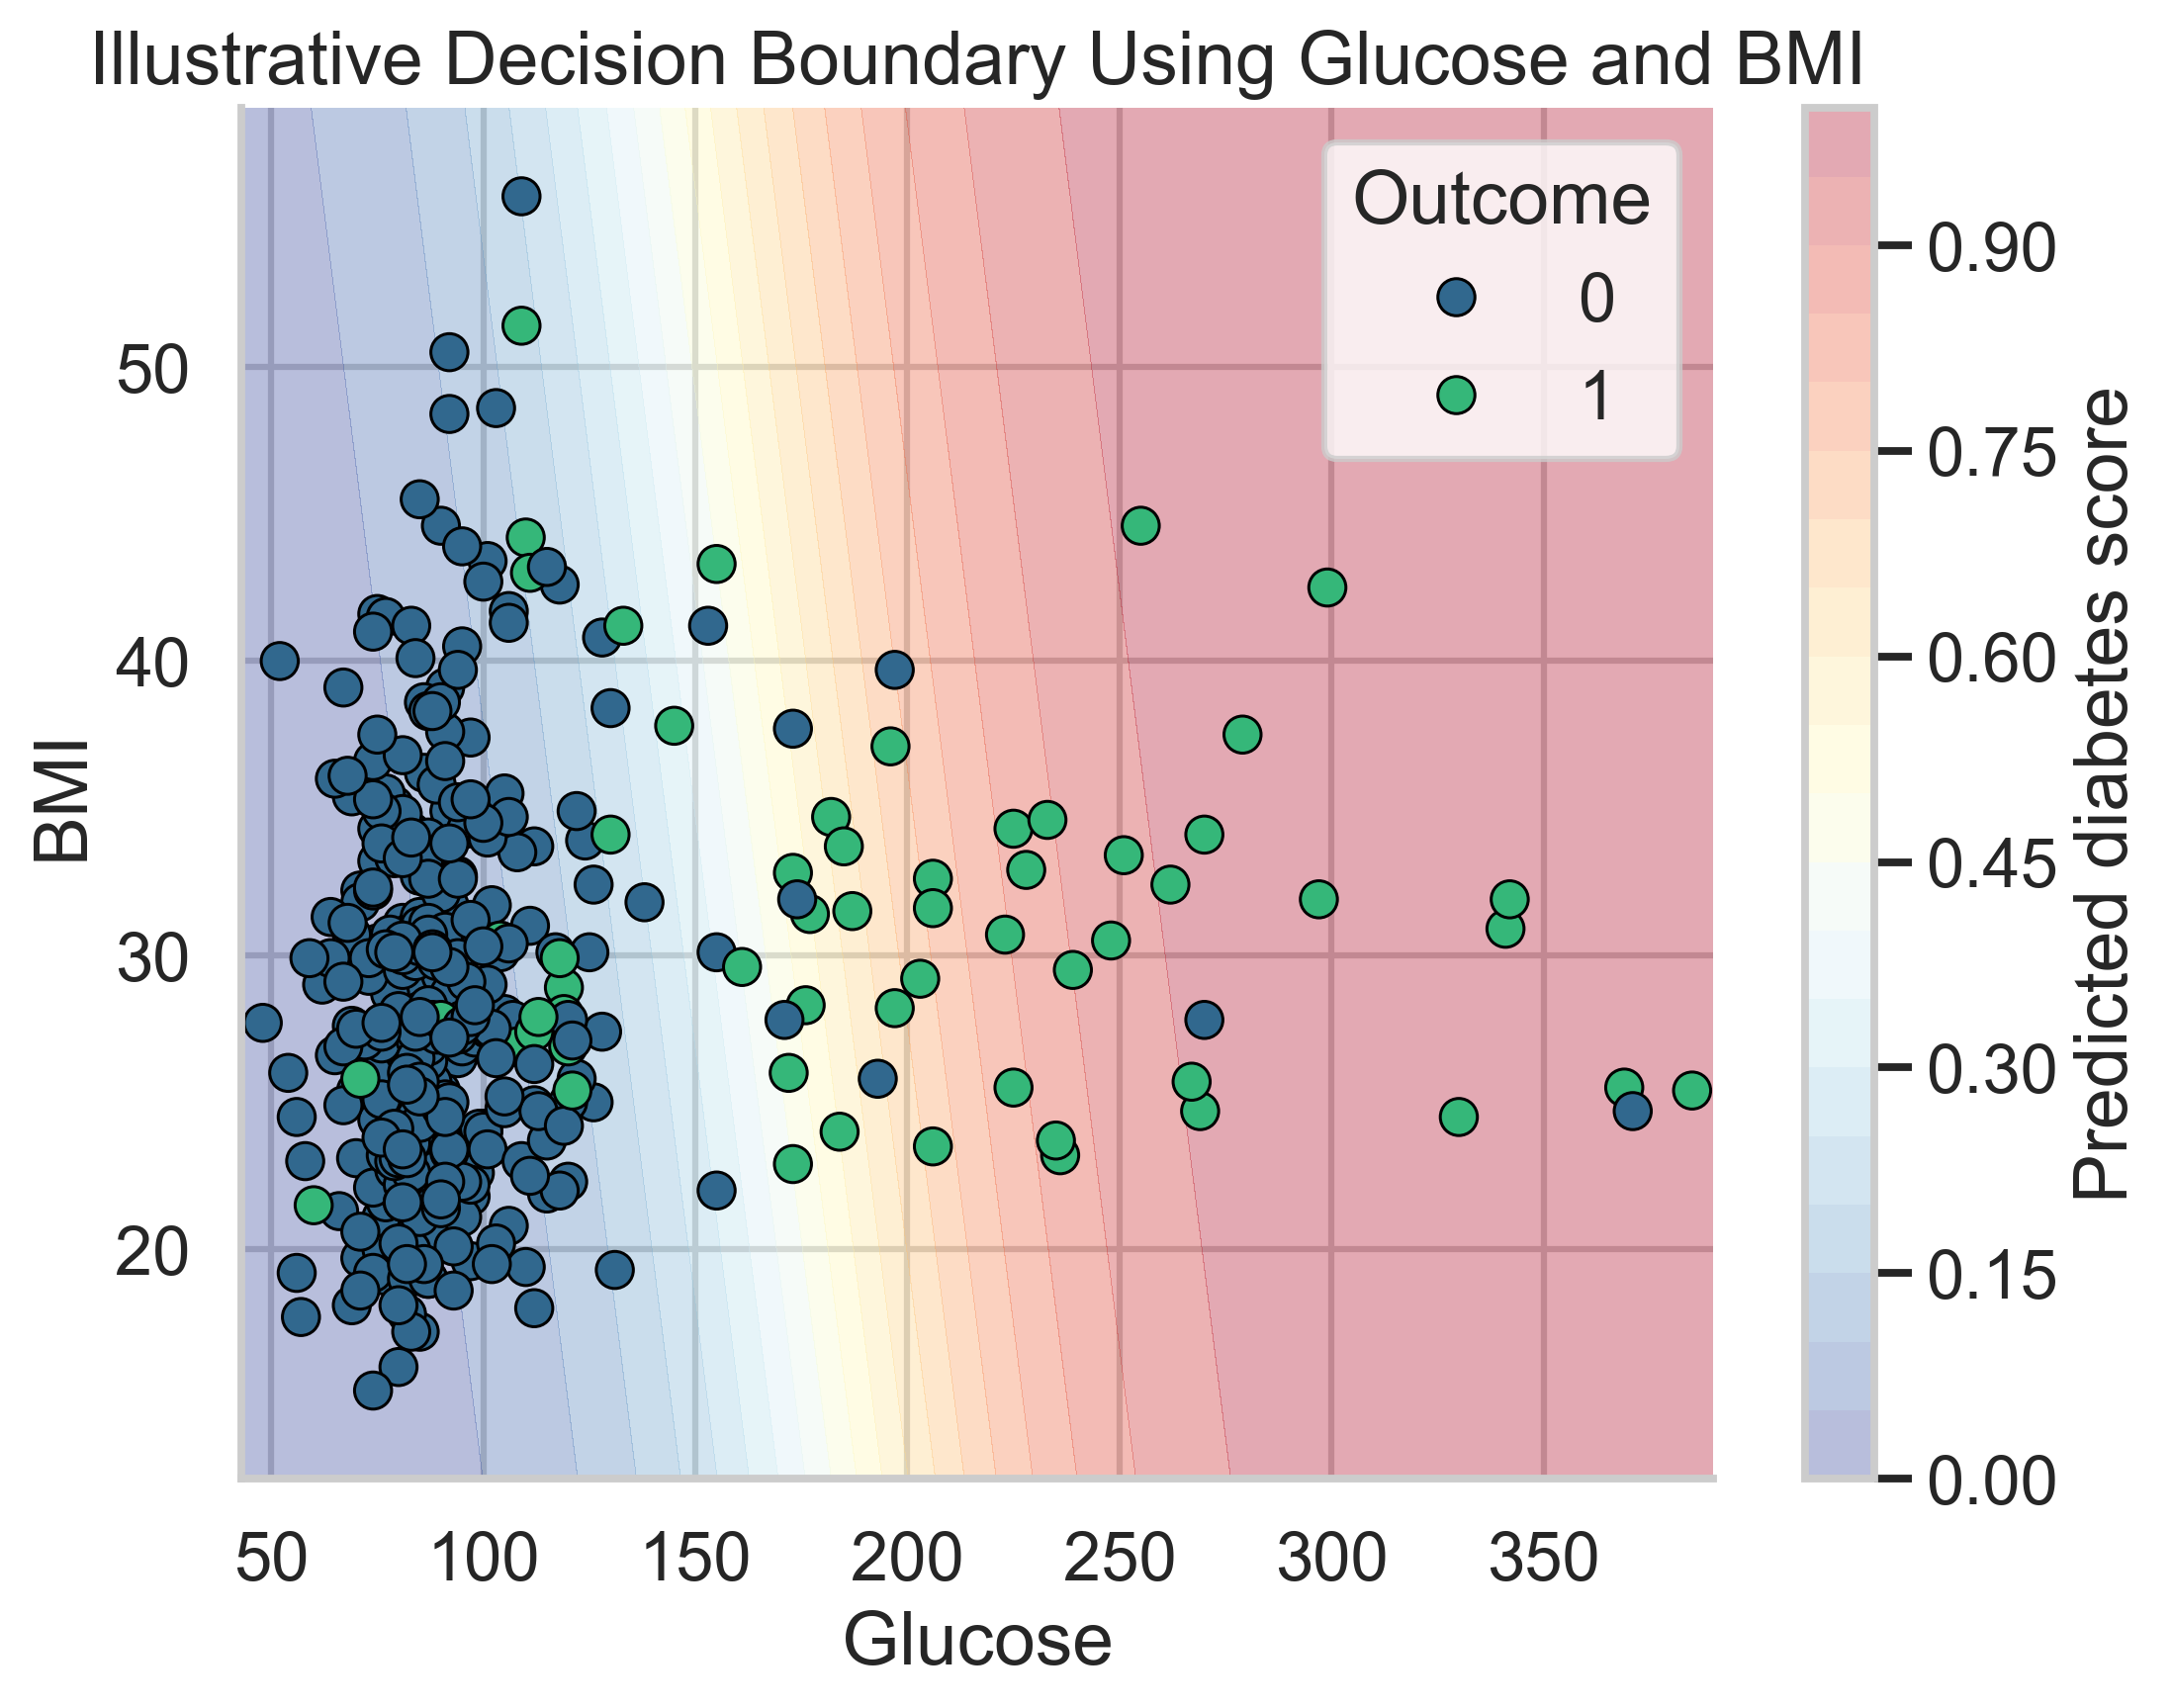
\includegraphics[width=0.82\linewidth]{classification_decision_boundary_glucose_bmi.png}
    \caption{Appendix decision-boundary projection using Glucose and BMI for a simplified two-feature view of the classification task.}
    \label{fig:appendix-decision-boundary}
\end{figure}

\begin{figure}[!t]
    \centering
    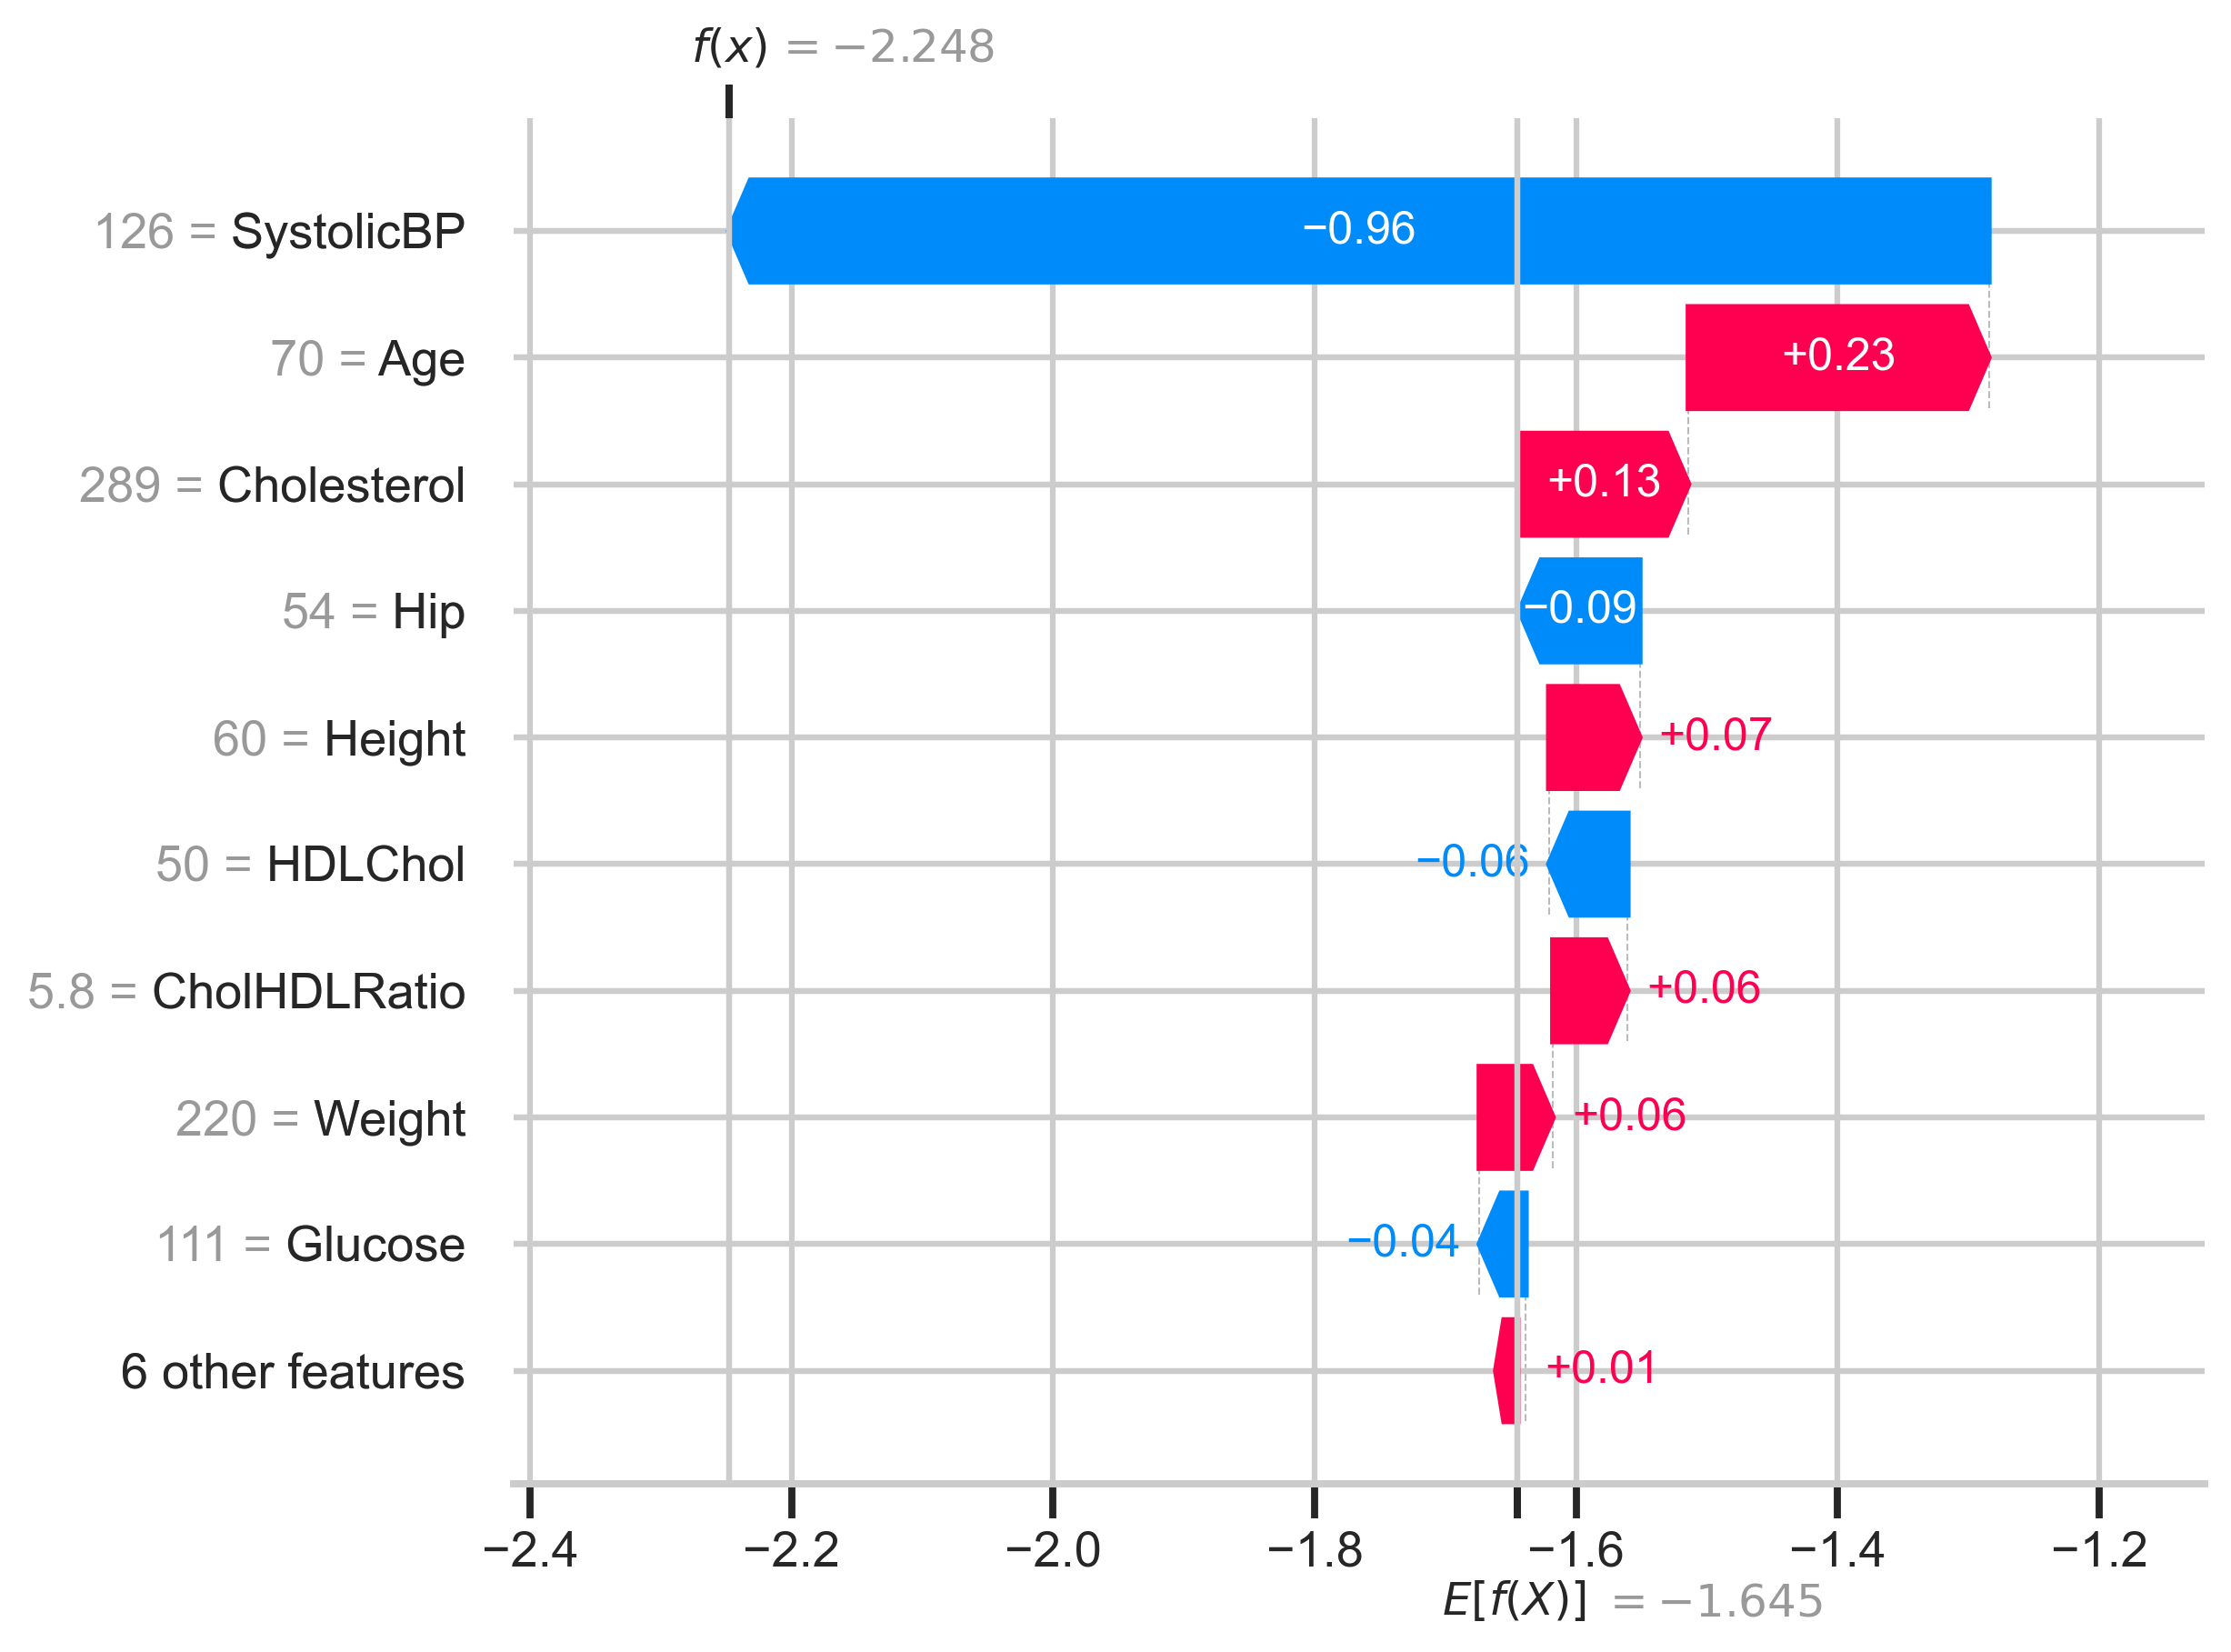
\includegraphics[width=0.82\linewidth]{shap_local_waterfall.png}
    \caption{Appendix local SHAP waterfall plot for an illustrative patient-level prediction.}
    \label{fig:appendix-waterfall}
\end{figure}

\end{document}
